\documentclass[]{report}

\usepackage{psfrag}
\usepackage{amsmath}
\usepackage{amssymb}
\usepackage{pstricks, pst-node, pst-plot, pst-circ}
\usepackage{moredefs}
\usepackage{hyperref}
\usepackage{cleveref}
\usepackage{graphicx}
\usepackage{epstopdf}
\usepackage{epsfig}
\usepackage{algorithm}
\usepackage{program}

% Title Page
\title{ Homework 3-4 Solution \\ \centering of \\ \centering Optimization in Engineering Class\\ \centering (MECH601)}
\author{MSc. Burak ER}

\begin{document}
\maketitle

\begin{abstract}
Solved problems in this homework are some of the problems at the end of chapter 4, 10 and 11 of the book Introduction to Optimum Design by Jasbir Arora\cite{arora2004introduction}. The solution includes the following problems; Problem 4.7, 4.9, 4.22, 4.32, 4.47, 4.60, 4.85, 4.101, 4.138, 4.150, 8.11, 8.16, 8.27, 8.53, 8.59, 8.68, 9.10, 9.12, 9.33.
\end{abstract}
\subsection*{Problem 4.7}
Write down the Taylor Series representation of $e^x$ including quadratic terms around $x^*=2$.
\subsubsection*{Solution}
Taylor series of any function around $x_0$ is given by
\begin{eqnarray}
f\left(x_0+\Delta x\right)&=&x_0+f^\prime\left(x_0\right)\Delta x+\frac{f^{\prime \prime}\left(x\right)}{2!}\left(\Delta x\right)^2+\dots
\end{eqnarray}
by putting $\Delta x=x-x_0$ and neglecting the higher order terms, it is found that
\begin{eqnarray*}
f\left(x\right)&=&2+e^2\left(x-2\right)+\frac{e^2}{2!}\left(x-2\right)^2 \\
&=&2+e^2\left(\frac{x^2}{2}-x\right)
\end{eqnarray*}
Therefore, Taylor series of $e^x$ around the point $x^*=2$ is found as
\begin{eqnarray*}
f\left(x\right)&=& e^2\left(\frac{x^2}{2}-x\right)+2
\end{eqnarray*}
\subsection*{Problem 4.9}
Determine the nature of the following quadratic form.
\begin{eqnarray}
F\left(\mathbf{x}\right)&=&x_1^2+4x_1x_2+2x_1x_3-7x_2^2-6x_2x_3+5x_3^2
\label{eqproblem:4.9}
\end{eqnarray}
\subsubsection*{Solution}
The quadratic form of the equation can be written as
\begin{eqnarray*}
F\left(\mathbf{x}\right)&=&\mathbf{x}^T\mathbf{P}\mathbf{x}
\end{eqnarray*}
\begin{eqnarray*}
\mathbf{x}&=&\left[x_1 \  x_2 \  x_3\right]^T
\end{eqnarray*}
\begin{eqnarray*}
\mathbf{P}&=&\left[\begin{array}{ccc}
1& 4& 2 \\
0& -7& -6\\
0& 0& 5
\end{array}\right]
\end{eqnarray*}
we can now determine the definition of the matrix $\mathbf{P}$ by finding the eigen values of it.
\begin{eqnarray*}
\mathrm{det}\left(\mathbf{P}-\lambda \mathbf{I}\right)&=&\mathrm{det}\left(\left[\begin{array}{ccc}
1-\lambda& 4& 2 \\
0& -7-\lambda& -6\\
0& 0& 5-\lambda
\end{array}\right]\right)=0
\end{eqnarray*}
From this determinant eigen value equation is found as
\begin{eqnarray*}
\left(-1\right)^2\left(1-\lambda\right)\left(-7-\lambda\right)\left(5-\lambda\right)+\left(-1\right)^3\left(4\right)\left(0\right)\left(0\right)+\left(-1\right)^4\left(2\right)\left(0\right)\left(0\right)&=&0
\end{eqnarray*}
or
\begin{eqnarray*}
\left(1-\lambda\right)\left(-7-\lambda\right)\left(5-\lambda\right)&=&0
\end{eqnarray*}
The eigen values of the $\mathbf{P}$ are $\lambda_1=1$ , $\lambda_2=-7$ , $\lambda_3=5$, thus, it is indefinite because of having at least one negative eigen value. Therefore, the function in equation \ref{eqproblem:4.9} is not convex.
\subsection*{Problem 4.22}
Find the stationary points for the following function. Also, determine the local minimum, local maximum and inflection points.
\begin{eqnarray}
f\left(\mathbf{x}\right)&=&3x_1^2+2x_1x_2+2x_2^2+7
\label{eqproblem:4.22}
\end{eqnarray}
\subsubsection*{Solution}
The function is written in quadratic form as
\begin{eqnarray*}
f\left(\mathbf{x}\right)&=&\mathbf{x}^T\mathbf{P}\mathbf{x}+\mathbf{b}
\label{eqproblem:4.22}
\end{eqnarray*}
\begin{eqnarray*}
\mathbf{x}&=&\left[\ x_1 \  x_2 \ \right]^T
\end{eqnarray*}
\begin{eqnarray*}
\mathbf{P}&=&\left[\begin{array}{ccc}
3& 2 \\
0& 2\\
\end{array}\right]
\end{eqnarray*}
\begin{eqnarray*}
\mathbf{b}&=&\left[\ 0 \  7 \ \right]^T
\end{eqnarray*}
stationary points is of the function is found by setting it's variation to zero
\begin{eqnarray*}
\delta{ f \left(\mathbf{x}\right)} &=& 0 \\
&=& 2\delta{\mathbf{x}}^T\mathbf{P}\mathbf{x}
\end{eqnarray*}
by setting $\delta \mathbf{x}$ arbitrary it is found
\begin{eqnarray*}
\mathbf{P}\mathbf{x}=0
\end{eqnarray*}
Resulting two linear equations
\begin{eqnarray*}
6x_1+2x_2=0\\
4x_2=0
\end{eqnarray*}
$x_1$ and $x_2$ is found
\begin{eqnarray*}
x_1=0\\
x_2=0
\end{eqnarray*}
From the definition $\mathbf H=2\mathbf{P}$. The eigen values of $\mathbf H$;
\begin{eqnarray*}
\mathrm{det}\left(\mathbf{H}-\lambda \mathbf{I}\right)&=&\mathrm{det}\left(\left[\begin{array}{cc}
6-\lambda& 4\\
0& 4-\lambda
\end{array}\right]\right)=0
\end{eqnarray*}
\begin{eqnarray*}
\left(6-\lambda\right) \left(4-\lambda\right)=0 \Longrightarrow \lambda_1=6 \ , \lambda_2=4
\end{eqnarray*}
Eigen values of Hessian matrix are both positive thus it is positive definite. Therefore, the point $\mathbf x=\left(0,0\right)$ is a global minimum.
\subsection*{Problem 4.32}
Annual operating cost U for an electrical line system is given by the following expression
\begin{eqnarray}
\mathrm U&=&\frac{21.9\times 10^7}{\mathrm V^2 \mathrm C}+3.9\times 10^6 \mathrm C+1000 \mathrm V 
\end{eqnarray}
\begin{eqnarray*}
\begin{array}{l}
\mathrm{V:line \ voltage}\ ,\ \mathrm{C:line \ capacitance}
\end{array}
\end{eqnarray*}
Find the stationary points for the function and determine V and C to minimize the operating cost.
\subsubsection*{Solution}
At stationary points, variation of function is equal to zero, thus,
\begin{eqnarray*}
\delta \mathrm U &=&\frac{\partial \mathrm U}{\partial \mathbf x} \delta \mathbf{x} =0
\end{eqnarray*}
\begin{eqnarray*}
\delta \mathrm U &=&\left[\frac{43.8\times 10^7}{\mathrm V^3 \mathrm C}+1000 \ \ - \frac{21.9\times 10^7}{\mathrm V^2 \mathrm C^2}+3.9\times 10^6\right] \left[\begin{array}{c}\delta \mathrm V \\ \delta \mathrm C \end{array}\right]
\end{eqnarray*}
the stationary points should satisfy the equations
\begin{eqnarray*}
\frac{43.8\times 10^7}{\mathrm V^3 \mathrm C}+1000 &=&0 \\
- \frac{21.9\times 10^7}{\mathrm V^2 \mathrm C^2}+3.9\times 10^6 &=&0 \\
\end{eqnarray*}
Using Newton-Raphson method for the solution of this two equations, stationary point of the function is found at
\begin{eqnarray*}
\mathrm V &=& 241.764 \mathrm {kV} \\
\mathrm C &=& 0.031 \mathrm {mhos}
\end{eqnarray*}
This value is just a stationary point. Determining whether it is a min or max requires Hessian matrix to be evaluated. Hessian of the function is
\begin{eqnarray*}
\mathbf H &=& \left[ \begin{array}{cc}
\frac{\partial^2 \mathrm U}{\partial  V^2} &\frac{\partial^2 \mathrm U}{\partial \mathrm V \partial \mathrm C}\\
\frac{\partial^2 \mathrm U}{\partial \mathrm V \partial \mathrm C} & \frac{\partial^2 \mathrm U}{\partial \mathrm C^2}
\end{array}\right]
\end{eqnarray*}
Evaluating at stationary point \textbf{H} is found as
\begin{eqnarray*}
\mathbf H &=& \left[ \begin{array}{cc}
12.408 &32262.9502\\
32262.9502 & 2.516\times10^8
\end{array}\right]
\end{eqnarray*}
Eigen values of the Hessian matrix are found as $\lambda_1 >0\;\&\;\lambda_2 >0$, thus, it is positive definite which makes the stationary point \underline{minimum}.
\subsection*{Problem 4.47}
Minimize:
\begin{eqnarray*}
f\left(\mathbf x\right) &=& 4 x_1^2+9x_2^2+6x_2-4x_1+13
\end{eqnarray*} 
Subject to:
\begin{eqnarray*}
x_1-3x_2+3&=& 0
\end{eqnarray*} 
\subsubsection*{Solution}
The function to be minimized includes only equality constraint. It can be solved analytically by using Lagrange Multipliers Method. Minimization of the problem function with constraints is equivalent to minimization of Lagrangian. Lagrangian of a problem is given as
\begin{eqnarray*}
L\left(\mathbf{x}\right)=f\left(\mathbf{x}\right)+\mathbf{v}^T \mathbf{h}\left(\mathbf x\right)
\end{eqnarray*}
Lagrangian of the problem is found as
\begin{eqnarray*}
L\left(\mathbf{x}\right)=4 x_1^2+9x_2^2+6x_2-4x_1+13+v_1\left(x_1-3x_2+3\right)
\end{eqnarray*}
Stationary point of the Lagrangian is found as
\begin{eqnarray*}
\delta L\left(\mathbf{x}\right)=\left(8 x_1-4\right)\delta x_1+\left(18x_2+6-3v_1\right)\delta x_2+v_1\left(x_1-3x_2+3\right)\delta v_1=0
\end{eqnarray*}
For arbitrary variations, this results to three equations with three unknowns as
\begin{eqnarray*}
8x_1-4+v_1&=& 0\\
18x_2+6-3v_1&=& 0\\
x_1-3x_2+3&=& 0\\
\end{eqnarray*}
Solution of this equations is $x_1=0.4$ , $x_2=1.133$ and $v_1=8.798$.
\subsection*{Problem 4.60}
Minimize:
\begin{eqnarray*}
f\left(\mathbf x\right) &=& \left(x-4\right)^2+\left(y-6\right)^2
\end{eqnarray*} 
Subject to:
\begin{eqnarray*}
12 &\geq& x+y \\
x &\geq& 6  \\
y &\geq& 0
\end{eqnarray*} 
\subsubsection*{Solution}
The problem can be solved by Lagrange Multipliers method. It includes three inequality constraints. Lagrangian of a problem with both equality and inequality constraints is given by 
\begin{eqnarray*}
L &=&f\left(\mathbf x\right) + \mathbf{v}^T\mathbf{h}+\mathbf{u}^T\left(\mathbf{g}+\mathbf{s}^2\right)
\end{eqnarray*}
\begin{eqnarray*}
L&=&\left(x-4\right)^2+\left(y-6\right)^2+0+u_1\left(x+y-12+s_1^2\right)+u_2\left(6-x+s_2^2\right)+u_3\left(-y+s_3^2\right)
\end{eqnarray*}
Lagrangian should be stationary for an extremum value 
\begin{eqnarray*}
\delta L &=&0
\end{eqnarray*}
\begin{eqnarray*}
\delta L &=& \left(2\left(x-4\right)+u_1-u_2\right) \delta x +\left(2\left(y-2\right)+u_1-u_3\right)\delta y+\\
&&\left(x+y-12+s_1^2\right)\delta u_1+\left(6-x+s_2^2\right)\delta u_2+\\
&&\left(-y+s_3^2\right)\delta u_3+\left(x+y-12+s_1^2\right)\delta s_1+\\
&&\left(x+y-12+s_1^2\right)\delta s_2+\left(x+y-12+s_1^2\right)\delta s_3
\end{eqnarray*}
This condition results eight independent nonlinear equations with eight unknowns as
\begin{eqnarray*}
2\left(x-4\right)+u_1-u_2&=&0\\
2\left(y-6\right)+u_1-u_3&=&0\\
x+y-12+s_1^2&=&0\\
6-x+s_2^2&=&0\\
-y+s_3^2&=&0\\
2s_1u_1&=&0\\
2s_2u_2&=&0\\
2s_3u_3&=&0\\
\end{eqnarray*}
solving these nonlinear equations results the following values,
\begin{eqnarray*}
\begin{array}{lc}
 x=6\;,\;y=6\;,\;u_1=4.3e^{-19}\;,\;u_2=4\;,\;u_3=4.028e^{-19}\;,\;s_1=5.63e^{-19}\;,&\\ \;s_2=4.49e^{-19}\;,\;s_3=2.4495e^{-19}&
 \end{array}
\end{eqnarray*}
\subsection*{Problem 4.85}
Formulate and solve the following problem graphically.Verify the KKT condtions at the solution point and show the gradients of the cost function and active constraints on the graph.\\
~
\\
Minimize:
\begin{eqnarray*}
f\left(x,y\right) &=& -\pi x^2 y
\end{eqnarray*} 
Subject to:
\begin{eqnarray*}
x-20 &\leq& 0 \\
y-20 &\leq& 0\\
5-x &\leq& 0\\
-x &\leq& 0\\
2\pi x y -900 &\leq& 0
\end{eqnarray*} 
\subsubsection{Solution}
Graphical solution is given in \cref{fig:problem485}.
\begin{figure}[ht!]
% This file has been created by Matfig2PGF v0.3.9
\begin{pgfpicture}
  % Axes
  \begin{pgfscope}
    \definecolor{matfig2pgf_color}{rgb}{1,1,1}\pgfsetfillcolor{matfig2pgf_color}
    \pgfpathrectangle{\pgfpoint{3.57404cm}{2.68053cm}}{\pgfpoint{21.039cm}{12.5469cm}}
    \pgfusepath{fill}
  \end{pgfscope}
  % X tick marks
  \begin{pgfscope}
    \pgfsetlinewidth{0.5pt}
    \definecolor{matfig2pgf_linecolor}{rgb}{0.000,0.000,0.000}
    \pgfsetstrokecolor{matfig2pgf_linecolor}
    \foreach \x in {6.20391,8.83378,11.4637,14.0935,16.7234,19.3533,21.9831}
    {
      \pgfpathmoveto{\pgfpoint{\x cm}{2.68053cm}}\pgfpathlineto{\pgfpoint{\x cm}{2.806cm}}
      \pgfpathmoveto{\pgfpoint{\x cm}{15.2274cm}}\pgfpathlineto{\pgfpoint{\x cm}{15.102cm}}
    }
    \pgfusepath{stroke}
  \end{pgfscope}
  % Y tick marks
  \begin{pgfscope}
    \pgfsetlinewidth{0.5pt}
    \definecolor{matfig2pgf_linecolor}{rgb}{0.000,0.000,0.000}
    \pgfsetstrokecolor{matfig2pgf_linecolor}
    \foreach \y in {3.93522,5.18991,6.4446,7.69929,8.95399,10.2087,11.4634,12.7181,13.9728}
    {
      \pgfpathmoveto{\pgfpoint{3.57404cm}{\y cm}}\pgfpathlineto{\pgfpoint{3.78443cm}{\y cm}}
      \pgfpathmoveto{\pgfpoint{24.613cm}{\y cm}}\pgfpathlineto{\pgfpoint{24.4026cm}{\y cm}}
    }
    \pgfusepath{stroke}
  \end{pgfscope}
  % Outer axes line
  \begin{pgfscope}
    \pgfsetlinewidth{0.5pt}
    \pgfpathrectangle{\pgfpoint{3.57404cm}{2.68053cm}}{\pgfpoint{21.039cm}{12.5469cm}}
    \pgfusepath{stroke}
  \end{pgfscope}
  % Tick labels
  \begin{pgfscope}
    \definecolor{matfig2pgf_fillcolor}{rgb}{0.000,0.000,0.000}
    \pgfsetfillcolor{matfig2pgf_fillcolor}
    \pgftext[x=3.57404cm,y=2.58053cm,top]{$-10$}
    \pgftext[x=6.20391cm,y=2.58053cm,top]{$-5$}
    \pgftext[x=8.83378cm,y=2.58053cm,top]{$0$}
    \pgftext[x=11.4637cm,y=2.58053cm,top]{$5$}
    \pgftext[x=14.0935cm,y=2.58053cm,top]{$10$}
    \pgftext[x=16.7234cm,y=2.58053cm,top]{$15$}
    \pgftext[x=19.3533cm,y=2.58053cm,top]{$20$}
    \pgftext[x=21.9831cm,y=2.58053cm,top]{$25$}
    \pgftext[x=24.613cm,y=2.58053cm,top]{$30$}
  \end{pgfscope}
  \begin{pgfscope}
    \definecolor{matfig2pgf_fillcolor}{rgb}{0.000,0.000,0.000}
    \pgfsetfillcolor{matfig2pgf_fillcolor}
    \pgftext[x=3.47404cm,y=2.68053cm,right]{$-20$}
    \pgftext[x=3.47404cm,y=3.93522cm,right]{$-15$}
    \pgftext[x=3.47404cm,y=5.18991cm,right]{$-10$}
    \pgftext[x=3.47404cm,y=6.4446cm,right]{$-5$}
    \pgftext[x=3.47404cm,y=7.69929cm,right]{$0$}
    \pgftext[x=3.47404cm,y=8.95399cm,right]{$5$}
    \pgftext[x=3.47404cm,y=10.2087cm,right]{$10$}
    \pgftext[x=3.47404cm,y=11.4634cm,right]{$15$}
    \pgftext[x=3.47404cm,y=12.7181cm,right]{$20$}
    \pgftext[x=3.47404cm,y=13.9728cm,right]{$25$}
    \pgftext[x=3.47404cm,y=15.2274cm,right]{$30$}
  \end{pgfscope}
  % Patch object
  \begin{pgfscope}
    \pgfsetlinewidth{2.00pt}
    \definecolor{matfig2pgf_linecolor}{rgb}{0.000,0.000,0.000}
    \pgfsetstrokecolor{matfig2pgf_linecolor}
    \pgfsetdash{}{0pt}
    \definecolor{matfig2pgf_facecolor}{rgb}{0.9375,1,0.0625}\pgfsetfillcolor{matfig2pgf_facecolor}
    \pgfplothandlerlineto
\pgfplotstreamstart
\foreach \x/\y in {24.613/15.227,24.613/15.227,24.613/15.202,24.613/15.177,24.613/15.152,24.613/15.127,24.613/15.102,24.613/15.077,24.613/15.052
,24.613/15.027,24.613/15.002,24.613/14.977,24.613/14.951,24.613/14.926,24.613/14.901,24.613/14.876,24.613/14.851,24.613/14.826,24.613/14.801
,24.613/14.776,24.613/14.751,24.613/14.726,24.613/14.700,24.613/14.675,24.613/14.650,24.613/14.625,24.613/14.600,24.613/14.575,24.613/14.550
,24.613/14.525,24.613/14.500,24.613/14.475,24.613/14.450,24.613/14.424,24.613/14.399,24.613/14.374,24.613/14.349,24.613/14.324,24.613/14.299
,24.613/14.274,24.613/14.249,24.613/14.224,24.613/14.199,24.613/14.174,24.613/14.148,24.613/14.123,24.613/14.098,24.613/14.073,24.613/14.048
,24.613/14.023,24.613/13.998,24.613/13.973,24.613/13.948,24.613/13.923,24.613/13.897,24.613/13.872,24.613/13.847,24.613/13.822,24.613/13.797
,24.613/13.772,24.613/13.747,24.613/13.722,24.613/13.697,24.613/13.672,24.613/13.647,24.613/13.621,24.613/13.596,24.613/13.571,24.613/13.546
,24.613/13.521,24.613/13.496,24.613/13.471,24.613/13.446,24.613/13.421,24.613/13.396,24.613/13.371,24.613/13.345,24.613/13.320,24.613/13.295
,24.613/13.270,24.613/13.245,24.613/13.220,24.613/13.195,24.613/13.170,24.613/13.145,24.613/13.120,24.613/13.094,24.613/13.069,24.613/13.044
,24.613/13.019,24.613/12.994,24.613/12.969,24.613/12.944,24.613/12.919,24.613/12.894,24.613/12.869,24.613/12.844,24.613/12.818,24.613/12.793
,24.613/12.768,24.613/12.743,24.613/12.718,24.613/12.693,24.613/12.668,24.613/12.643,24.613/12.618,24.613/12.593,24.613/12.567,24.613/12.542
,24.613/12.517,24.613/12.492,24.613/12.467,24.613/12.442,24.613/12.417,24.613/12.392,24.613/12.367,24.613/12.342,24.613/12.317,24.613/12.291
,24.613/12.266,24.613/12.241,24.613/12.216,24.613/12.191,24.613/12.166,24.613/12.141,24.613/12.116,24.613/12.091,24.613/12.066,24.613/12.041
,24.613/12.015,24.613/11.990,24.613/11.965,24.613/11.940,24.613/11.915,24.613/11.890,24.613/11.865,24.613/11.840,24.613/11.815,24.613/11.790
,24.613/11.764,24.613/11.739,24.613/11.714,24.613/11.689,24.613/11.664,24.613/11.639,24.613/11.614,24.613/11.589,24.613/11.564,24.613/11.539
,24.613/11.514,24.613/11.488,24.613/11.463,24.613/11.438,24.613/11.413,24.613/11.388,24.613/11.363,24.613/11.338,24.613/11.313,24.613/11.288
,24.613/11.263,24.613/11.238,24.613/11.212,24.613/11.187,24.613/11.162,24.613/11.137,24.613/11.112,24.613/11.087,24.613/11.062,24.613/11.037
,24.613/11.012,24.613/10.987,24.613/10.961,24.613/10.936,24.613/10.911,24.613/10.886,24.613/10.861,24.613/10.836,24.613/10.811,24.613/10.786
,24.613/10.761,24.613/10.736,24.613/10.711,24.613/10.685,24.613/10.660,24.613/10.635,24.613/10.610,24.613/10.585,24.613/10.560,24.613/10.535
,24.613/10.510,24.613/10.485,24.613/10.460,24.613/10.435,24.613/10.409,24.613/10.384,24.613/10.359,24.613/10.334,24.613/10.309,24.613/10.284
,24.613/10.259,24.613/10.234,24.613/10.209,24.613/10.184,24.613/10.158,24.613/10.133,24.613/10.108,24.613/10.083,24.613/10.058,24.613/10.033
,24.613/10.008,24.613/9.983,24.613/9.958,24.613/9.933,24.613/9.908,24.613/9.882,24.613/9.857,24.613/9.832,24.613/9.807,24.613/9.782
,24.613/9.757,24.613/9.732,24.613/9.707,24.613/9.682,24.613/9.657,24.613/9.632,24.613/9.606,24.613/9.581,24.613/9.556,24.613/9.531
,24.613/9.506,24.613/9.481,24.613/9.456,24.613/9.431,24.613/9.406,24.613/9.381,24.613/9.355,24.613/9.330,24.613/9.305,24.613/9.280
,24.613/9.255,24.613/9.230,24.613/9.205,24.613/9.180,24.613/9.155,24.613/9.130,24.613/9.105,24.613/9.079,24.613/9.054,24.613/9.029
,24.613/9.004,24.613/8.979,24.613/8.954,24.613/8.929,24.613/8.904,24.613/8.879,24.613/8.854,24.613/8.829,24.613/8.803,24.613/8.778
,24.613/8.753,24.613/8.728,24.613/8.703,24.613/8.678,24.613/8.653,24.613/8.628,24.613/8.603,24.613/8.578,24.613/8.552,24.613/8.527
,24.613/8.502,24.613/8.477,24.613/8.452,24.613/8.427,24.613/8.402,24.613/8.377,24.613/8.352,24.613/8.327,24.613/8.302,24.613/8.276
,24.613/8.251,24.613/8.226,24.613/8.201,24.613/8.176,24.613/8.151,24.613/8.126,24.613/8.101,24.613/8.076,24.613/8.051,24.613/8.026
,24.613/8.000,24.613/7.975,24.613/7.950,24.613/7.925,24.613/7.900,24.613/7.875,24.613/7.850,24.613/7.825,24.613/7.800,24.613/7.775
,24.613/7.749,24.613/7.724,24.613/7.699,24.613/7.674,24.613/7.649,24.613/7.624,24.613/7.599,24.613/7.574,24.613/7.549,24.613/7.524
,24.613/7.499,24.613/7.473,24.613/7.448,24.613/7.423,24.613/7.398,24.613/7.373,24.613/7.348,24.613/7.323,24.613/7.298,24.613/7.273
,24.613/7.248,24.613/7.223,24.613/7.197,24.613/7.172,24.613/7.147,24.613/7.122,24.613/7.097,24.613/7.072,24.613/7.047,24.613/7.022
,24.613/6.997,24.613/6.972,24.613/6.946,24.613/6.921,24.613/6.896,24.613/6.871,24.613/6.846,24.613/6.821,24.613/6.796,24.613/6.771
,24.613/6.746,24.613/6.721,24.613/6.696,24.613/6.670,24.613/6.645,24.613/6.620,24.613/6.595,24.613/6.570,24.613/6.545,24.613/6.520
,24.613/6.495,24.613/6.470,24.613/6.445,24.613/6.420,24.613/6.394,24.613/6.369,24.613/6.344,24.613/6.319,24.613/6.294,24.613/6.269
,24.613/6.244,24.613/6.219,24.613/6.194,24.613/6.169,24.613/6.143,24.613/6.118,24.613/6.093,24.613/6.068,24.613/6.043,24.613/6.018
,24.613/5.993,24.613/5.968,24.613/5.943,24.613/5.918,24.613/5.893,24.613/5.867,24.613/5.842,24.613/5.817,24.613/5.792,24.613/5.767
,24.613/5.742,24.613/5.717,24.613/5.692,24.613/5.667,24.613/5.642,24.613/5.617,24.613/5.591,24.613/5.566,24.613/5.541,24.613/5.516
,24.613/5.491,24.613/5.466,24.613/5.441,24.613/5.416,24.613/5.391,24.613/5.366,24.613/5.340,24.613/5.315,24.613/5.290,24.613/5.265
,24.613/5.240,24.613/5.215,24.613/5.190,24.613/5.165,24.613/5.140,24.613/5.115,24.613/5.090,24.613/5.064,24.613/5.039,24.613/5.014
,24.613/4.989,24.613/4.964,24.613/4.939,24.613/4.914,24.613/4.889,24.613/4.864,24.613/4.839,24.613/4.814,24.613/4.788,24.613/4.763
,24.613/4.738,24.613/4.713,24.613/4.688,24.613/4.663,24.613/4.638,24.613/4.613,24.613/4.588,24.613/4.563,24.613/4.537,24.613/4.512
,24.613/4.487,24.613/4.462,24.613/4.437,24.613/4.412,24.613/4.387,24.613/4.362,24.613/4.337,24.613/4.312,24.613/4.287,24.613/4.261
,24.613/4.236,24.613/4.211,24.613/4.186,24.613/4.161,24.613/4.136,24.613/4.111,24.613/4.086,24.613/4.061,24.613/4.036,24.613/4.011
,24.613/3.985,24.613/3.960,24.613/3.935,24.613/3.910,24.613/3.885,24.613/3.860,24.613/3.835,24.613/3.810,24.613/3.785,24.613/3.760
,24.613/3.734,24.613/3.709,24.613/3.684,24.613/3.659,24.613/3.634,24.613/3.609,24.613/3.584,24.613/3.559,24.613/3.534,24.613/3.509
,24.613/3.484,24.613/3.458,24.613/3.433,24.613/3.408,24.613/3.383,24.613/3.358,24.613/3.333,24.613/3.308,24.613/3.283,24.613/3.258
,24.613/3.233,24.613/3.207,24.613/3.182,24.613/3.157,24.613/3.132,24.613/3.107,24.613/3.082,24.613/3.057,24.613/3.032,24.613/3.007
,24.613/2.982,24.613/2.957,24.613/2.931,24.613/2.906,24.613/2.881,24.613/2.856,24.613/2.831,24.613/2.806,24.613/2.781,24.613/2.756
,24.613/2.731,24.613/2.706,24.613/2.681,24.613/2.681,24.560/2.681,24.508/2.681,24.455/2.681,24.403/2.681,24.350/2.681,24.297/2.681
,24.245/2.681,24.192/2.681,24.140/2.681,24.087/2.681,24.034/2.681,23.982/2.681,23.929/2.681,23.877/2.681,23.824/2.681,23.771/2.681
,23.719/2.681,23.666/2.681,23.614/2.681,23.561/2.681,23.508/2.681,23.456/2.681,23.403/2.681,23.351/2.681,23.298/2.681,23.245/2.681
,23.193/2.681,23.140/2.681,23.088/2.681,23.035/2.681,22.982/2.681,22.930/2.681,22.877/2.681,22.825/2.681,22.772/2.681,22.720/2.681
,22.667/2.681,22.614/2.681,22.562/2.681,22.509/2.681,22.457/2.681,22.404/2.681,22.351/2.681,22.299/2.681,22.246/2.681,22.194/2.681
,22.141/2.681,22.088/2.681,22.036/2.681,21.983/2.681,21.931/2.681,21.878/2.681,21.825/2.681,21.773/2.681,21.720/2.681,21.668/2.681
,21.615/2.681,21.562/2.681,21.510/2.681,21.457/2.681,21.405/2.681,21.352/2.681,21.299/2.681,21.247/2.681,21.194/2.681,21.142/2.681
,21.089/2.681,21.036/2.681,20.984/2.681,20.931/2.681,20.879/2.681,20.826/2.681,20.773/2.681,20.721/2.681,20.668/2.681,20.616/2.681
,20.563/2.681,20.510/2.681,20.458/2.681,20.405/2.681,20.353/2.681,20.300/2.681,20.247/2.681,20.195/2.681,20.142/2.681,20.090/2.681
,20.037/2.681,19.984/2.681,19.932/2.681,19.879/2.681,19.827/2.681,19.774/2.681,19.721/2.681,19.669/2.681,19.616/2.681,19.564/2.681
,19.511/2.681,19.458/2.681,19.406/2.681,19.353/2.681,19.353/2.706,19.353/2.731,19.353/2.756,19.353/2.781,19.353/2.806,19.353/2.831
,19.353/2.856,19.353/2.881,19.353/2.906,19.353/2.931,19.353/2.957,19.353/2.982,19.353/3.007,19.353/3.032,19.353/3.057,19.353/3.082
,19.353/3.107,19.353/3.132,19.353/3.157,19.353/3.182,19.353/3.207,19.353/3.233,19.353/3.258,19.353/3.283,19.353/3.308,19.353/3.333
,19.353/3.358,19.353/3.383,19.353/3.408,19.353/3.433,19.353/3.458,19.353/3.484,19.353/3.509,19.353/3.534,19.353/3.559,19.353/3.584
,19.353/3.609,19.353/3.634,19.353/3.659,19.353/3.684,19.353/3.709,19.353/3.734,19.353/3.760,19.353/3.785,19.353/3.810,19.353/3.835
,19.353/3.860,19.353/3.885,19.353/3.910,19.353/3.935,19.353/3.960,19.353/3.985,19.353/4.011,19.353/4.036,19.353/4.061,19.353/4.086
,19.353/4.111,19.353/4.136,19.353/4.161,19.353/4.186,19.353/4.211,19.353/4.236,19.353/4.261,19.353/4.287,19.353/4.312,19.353/4.337
,19.353/4.362,19.353/4.387,19.353/4.412,19.353/4.437,19.353/4.462,19.353/4.487,19.353/4.512,19.353/4.537,19.353/4.563,19.353/4.588
,19.353/4.613,19.353/4.638,19.353/4.663,19.353/4.688,19.353/4.713,19.353/4.738,19.353/4.763,19.353/4.788,19.353/4.814,19.353/4.839
,19.353/4.864,19.353/4.889,19.353/4.914,19.353/4.939,19.353/4.964,19.353/4.989,19.353/5.014,19.353/5.039,19.353/5.064,19.353/5.090
,19.353/5.115,19.353/5.140,19.353/5.165,19.353/5.190,19.353/5.215,19.353/5.240,19.353/5.265,19.353/5.290,19.353/5.315,19.353/5.340
,19.353/5.366,19.353/5.391,19.353/5.416,19.353/5.441,19.353/5.466,19.353/5.491,19.353/5.516,19.353/5.541,19.353/5.566,19.353/5.591
,19.353/5.617,19.353/5.642,19.353/5.667,19.353/5.692,19.353/5.717,19.353/5.742,19.353/5.767,19.353/5.792,19.353/5.817,19.353/5.842
,19.353/5.867,19.353/5.893,19.353/5.918,19.353/5.943,19.353/5.968,19.353/5.993,19.353/6.018,19.353/6.043,19.353/6.068,19.353/6.093
,19.353/6.118,19.353/6.143,19.353/6.169,19.353/6.194,19.353/6.219,19.353/6.244,19.353/6.269,19.353/6.294,19.353/6.319,19.353/6.344
,19.353/6.369,19.353/6.394,19.353/6.420,19.353/6.445,19.353/6.470,19.353/6.495,19.353/6.520,19.353/6.545,19.353/6.570,19.353/6.595
,19.353/6.620,19.353/6.645,19.353/6.670,19.353/6.696,19.353/6.721,19.353/6.746,19.353/6.771,19.353/6.796,19.353/6.821,19.353/6.846
,19.353/6.871,19.353/6.896,19.353/6.921,19.353/6.946,19.353/6.972,19.353/6.997,19.353/7.022,19.353/7.047,19.353/7.072,19.353/7.097
,19.353/7.122,19.353/7.147,19.353/7.172,19.353/7.197,19.353/7.223,19.353/7.248,19.353/7.273,19.353/7.298,19.353/7.323,19.353/7.348
,19.353/7.373,19.353/7.398,19.353/7.423,19.353/7.448,19.353/7.473,19.353/7.499,19.353/7.524,19.353/7.549,19.353/7.574,19.353/7.599
,19.353/7.624,19.353/7.649,19.353/7.674,19.353/7.699,19.353/7.724,19.353/7.749,19.353/7.775,19.353/7.800,19.353/7.825,19.353/7.850
,19.353/7.875,19.353/7.900,19.353/7.925,19.353/7.950,19.353/7.975,19.353/8.000,19.353/8.026,19.353/8.051,19.353/8.076,19.353/8.101
,19.353/8.126,19.353/8.151,19.353/8.176,19.353/8.201,19.353/8.226,19.353/8.251,19.353/8.276,19.353/8.302,19.353/8.327,19.353/8.352
,19.353/8.377,19.353/8.402,19.353/8.427,19.353/8.452,19.353/8.477,19.353/8.502,19.353/8.527,19.353/8.552,19.353/8.578,19.353/8.603
,19.353/8.628,19.353/8.653,19.353/8.678,19.353/8.703,19.353/8.728,19.353/8.753,19.353/8.778,19.353/8.803,19.353/8.829,19.353/8.854
,19.353/8.879,19.353/8.904,19.353/8.929,19.353/8.954,19.353/8.979,19.353/9.004,19.353/9.029,19.353/9.054,19.353/9.079,19.353/9.105
,19.353/9.130,19.353/9.155,19.353/9.180,19.353/9.205,19.353/9.230,19.353/9.255,19.353/9.280,19.353/9.305,19.353/9.330,19.353/9.355
,19.353/9.381,19.353/9.406,19.353/9.431,19.353/9.456,19.353/9.481,19.353/9.506,19.353/9.531,19.353/9.556,19.353/9.581,19.353/9.606
,19.353/9.632,19.353/9.657,19.353/9.682,19.353/9.707,19.353/9.732,19.353/9.757,19.353/9.782,19.353/9.807,19.353/9.832,19.353/9.857
,19.353/9.882,19.353/9.908,19.353/9.933,19.353/9.958,19.353/9.983,19.353/10.008,19.353/10.033,19.353/10.058,19.353/10.083,19.353/10.108
,19.353/10.133,19.353/10.158,19.353/10.184,19.353/10.209,19.353/10.234,19.353/10.259,19.353/10.284,19.353/10.309,19.353/10.334,19.353/10.359
,19.353/10.384,19.353/10.409,19.353/10.435,19.353/10.460,19.353/10.485,19.353/10.510,19.353/10.535,19.353/10.560,19.353/10.585,19.353/10.610
,19.353/10.635,19.353/10.660,19.353/10.685,19.353/10.711,19.353/10.736,19.353/10.761,19.353/10.786,19.353/10.811,19.353/10.836,19.353/10.861
,19.353/10.886,19.353/10.911,19.353/10.936,19.353/10.961,19.353/10.987,19.353/11.012,19.353/11.037,19.353/11.062,19.353/11.087,19.353/11.112
,19.353/11.137,19.353/11.162,19.353/11.187,19.353/11.212,19.353/11.238,19.353/11.263,19.353/11.288,19.353/11.313,19.353/11.338,19.353/11.363
,19.353/11.388,19.353/11.413,19.353/11.438,19.353/11.463,19.353/11.488,19.353/11.514,19.353/11.539,19.353/11.564,19.353/11.589,19.353/11.614
,19.353/11.639,19.353/11.664,19.353/11.689,19.353/11.714,19.353/11.739,19.353/11.764,19.353/11.790,19.353/11.815,19.353/11.840,19.353/11.865
,19.353/11.890,19.353/11.915,19.353/11.940,19.353/11.965,19.353/11.990,19.353/12.015,19.353/12.041,19.353/12.066,19.353/12.091,19.353/12.116
,19.353/12.141,19.353/12.166,19.353/12.191,19.353/12.216,19.353/12.241,19.353/12.266,19.353/12.291,19.353/12.317,19.353/12.342,19.353/12.367
,19.353/12.392,19.353/12.417,19.353/12.442,19.353/12.467,19.353/12.492,19.353/12.517,19.353/12.542,19.353/12.567,19.353/12.593,19.353/12.618
,19.353/12.643,19.353/12.668,19.353/12.693,19.353/12.718,19.353/12.743,19.353/12.768,19.353/12.793,19.353/12.818,19.353/12.844,19.353/12.869
,19.353/12.894,19.353/12.919,19.353/12.944,19.353/12.969,19.353/12.994,19.353/13.019,19.353/13.044,19.353/13.069,19.353/13.094,19.353/13.120
,19.353/13.145,19.353/13.170,19.353/13.195,19.353/13.220,19.353/13.245,19.353/13.270,19.353/13.295,19.353/13.320,19.353/13.345,19.353/13.371
,19.353/13.396,19.353/13.421,19.353/13.446,19.353/13.471,19.353/13.496,19.353/13.521,19.353/13.546,19.353/13.571,19.353/13.596,19.353/13.621
,19.353/13.647,19.353/13.672,19.353/13.697,19.353/13.722,19.353/13.747,19.353/13.772,19.353/13.797,19.353/13.822,19.353/13.847,19.353/13.872
,19.353/13.897,19.353/13.923,19.353/13.948,19.353/13.973,19.353/13.998,19.353/14.023,19.353/14.048,19.353/14.073,19.353/14.098,19.353/14.123
,19.353/14.148,19.353/14.174,19.353/14.199,19.353/14.224,19.353/14.249,19.353/14.274,19.353/14.299,19.353/14.324,19.353/14.349,19.353/14.374
,19.353/14.399,19.353/14.424,19.353/14.450,19.353/14.475,19.353/14.500,19.353/14.525,19.353/14.550,19.353/14.575,19.353/14.600,19.353/14.625
,19.353/14.650,19.353/14.675,19.353/14.700,19.353/14.726,19.353/14.751,19.353/14.776,19.353/14.801,19.353/14.826,19.353/14.851,19.353/14.876
,19.353/14.901,19.353/14.926,19.353/14.951,19.353/14.977,19.353/15.002,19.353/15.027,19.353/15.052,19.353/15.077,19.353/15.102,19.353/15.127
,19.353/15.152,19.353/15.177,19.353/15.202,19.353/15.227,19.406/15.227,19.458/15.227,19.511/15.227,19.564/15.227,19.616/15.227,19.669/15.227
,19.721/15.227,19.774/15.227,19.827/15.227,19.879/15.227,19.932/15.227,19.984/15.227,20.037/15.227,20.090/15.227,20.142/15.227,20.195/15.227
,20.247/15.227,20.300/15.227,20.353/15.227,20.405/15.227,20.458/15.227,20.510/15.227,20.563/15.227,20.616/15.227,20.668/15.227,20.721/15.227
,20.773/15.227,20.826/15.227,20.879/15.227,20.931/15.227,20.984/15.227,21.036/15.227,21.089/15.227,21.142/15.227,21.194/15.227,21.247/15.227
,21.299/15.227,21.352/15.227,21.405/15.227,21.457/15.227,21.510/15.227,21.562/15.227,21.615/15.227,21.668/15.227,21.720/15.227,21.773/15.227
,21.825/15.227,21.878/15.227,21.931/15.227,21.983/15.227,22.036/15.227,22.088/15.227,22.141/15.227,22.194/15.227,22.246/15.227,22.299/15.227
,22.351/15.227,22.404/15.227,22.457/15.227,22.509/15.227,22.562/15.227,22.614/15.227,22.667/15.227,22.720/15.227,22.772/15.227,22.825/15.227
,22.877/15.227,22.930/15.227,22.982/15.227,23.035/15.227,23.088/15.227,23.140/15.227,23.193/15.227,23.245/15.227,23.298/15.227,23.351/15.227
,23.403/15.227,23.456/15.227,23.508/15.227,23.561/15.227,23.614/15.227,23.666/15.227,23.719/15.227,23.771/15.227,23.824/15.227,23.877/15.227
,23.929/15.227,23.982/15.227,24.034/15.227,24.087/15.227,24.140/15.227,24.192/15.227,24.245/15.227,24.297/15.227,24.350/15.227,24.403/15.227
,24.455/15.227,24.508/15.227,24.560/15.227,24.613/15.227}
{
\pgfplotstreampoint{\pgfpoint{\x cm}{\y cm}}
}
\pgfplotstreamend
    \pgfpathclose
    \pgfusepath{stroke,fill}
  \end{pgfscope}
  % Patch object
  \begin{pgfscope}
    \pgfsetlinewidth{2.00pt}
    \definecolor{matfig2pgf_linecolor}{rgb}{0.000,0.000,0.000}
    \pgfsetstrokecolor{matfig2pgf_linecolor}
    \pgfsetdash{}{0pt}
    \definecolor{matfig2pgf_facecolor}{rgb}{0.9375,1,0.0625}\pgfsetfillcolor{matfig2pgf_facecolor}
    \pgfplothandlerlineto
\pgfplotstreamstart
\foreach \x/\y in {3.574/15.227,3.627/15.227,3.679/15.227,3.732/15.227,3.784/15.227,3.837/15.227,3.890/15.227,3.942/15.227,3.995/15.227
,4.047/15.227,4.100/15.227,4.153/15.227,4.205/15.227,4.258/15.227,4.310/15.227,4.363/15.227,4.416/15.227,4.468/15.227,4.521/15.227
,4.573/15.227,4.626/15.227,4.679/15.227,4.731/15.227,4.784/15.227,4.836/15.227,4.889/15.227,4.942/15.227,4.994/15.227,5.047/15.227
,5.099/15.227,5.152/15.227,5.205/15.227,5.257/15.227,5.310/15.227,5.362/15.227,5.415/15.227,5.468/15.227,5.520/15.227,5.573/15.227
,5.625/15.227,5.678/15.227,5.731/15.227,5.783/15.227,5.836/15.227,5.888/15.227,5.941/15.227,5.994/15.227,6.046/15.227,6.099/15.227
,6.151/15.227,6.204/15.227,6.257/15.227,6.309/15.227,6.362/15.227,6.414/15.227,6.467/15.227,6.519/15.227,6.572/15.227,6.625/15.227
,6.677/15.227,6.730/15.227,6.782/15.227,6.835/15.227,6.888/15.227,6.940/15.227,6.993/15.227,7.045/15.227,7.098/15.227,7.151/15.227
,7.203/15.227,7.256/15.227,7.308/15.227,7.361/15.227,7.414/15.227,7.466/15.227,7.519/15.227,7.571/15.227,7.624/15.227,7.677/15.227
,7.729/15.227,7.782/15.227,7.834/15.227,7.887/15.227,7.940/15.227,7.992/15.227,8.045/15.227,8.097/15.227,8.150/15.227,8.203/15.227
,8.255/15.227,8.308/15.227,8.360/15.227,8.413/15.227,8.466/15.227,8.518/15.227,8.571/15.227,8.623/15.227,8.676/15.227,8.729/15.227
,8.781/15.227,8.834/15.227,8.886/15.227,8.939/15.227,8.992/15.227,9.044/15.227,9.097/15.227,9.149/15.227,9.202/15.227,9.255/15.227
,9.307/15.227,9.360/15.227,9.412/15.227,9.465/15.227,9.518/15.227,9.570/15.227,9.623/15.227,9.675/15.227,9.728/15.227,9.781/15.227
,9.833/15.227,9.886/15.227,9.938/15.227,9.991/15.227,10.044/15.227,10.096/15.227,10.149/15.227,10.201/15.227,10.254/15.227,10.307/15.227
,10.359/15.227,10.412/15.227,10.464/15.227,10.517/15.227,10.569/15.227,10.622/15.227,10.675/15.227,10.727/15.227,10.780/15.227,10.832/15.227
,10.885/15.227,10.938/15.227,10.990/15.227,11.043/15.227,11.095/15.227,11.148/15.227,11.201/15.227,11.253/15.227,11.306/15.227,11.358/15.227
,11.411/15.227,11.464/15.227,11.516/15.227,11.569/15.227,11.621/15.227,11.674/15.227,11.727/15.227,11.779/15.227,11.832/15.227,11.884/15.227
,11.937/15.227,11.990/15.227,12.042/15.227,12.095/15.227,12.147/15.227,12.200/15.227,12.253/15.227,12.305/15.227,12.358/15.227,12.410/15.227
,12.463/15.227,12.516/15.227,12.568/15.227,12.621/15.227,12.673/15.227,12.726/15.227,12.779/15.227,12.831/15.227,12.884/15.227,12.936/15.227
,12.989/15.227,13.042/15.227,13.094/15.227,13.147/15.227,13.199/15.227,13.252/15.227,13.305/15.227,13.357/15.227,13.410/15.227,13.462/15.227
,13.515/15.227,13.568/15.227,13.620/15.227,13.673/15.227,13.725/15.227,13.778/15.227,13.831/15.227,13.883/15.227,13.936/15.227,13.988/15.227
,14.041/15.227,14.094/15.227,14.146/15.227,14.199/15.227,14.251/15.227,14.304/15.227,14.357/15.227,14.409/15.227,14.462/15.227,14.514/15.227
,14.567/15.227,14.620/15.227,14.672/15.227,14.725/15.227,14.777/15.227,14.830/15.227,14.882/15.227,14.935/15.227,14.988/15.227,15.040/15.227
,15.093/15.227,15.145/15.227,15.198/15.227,15.251/15.227,15.303/15.227,15.356/15.227,15.408/15.227,15.461/15.227,15.514/15.227,15.566/15.227
,15.619/15.227,15.671/15.227,15.724/15.227,15.777/15.227,15.829/15.227,15.882/15.227,15.934/15.227,15.987/15.227,16.040/15.227,16.092/15.227
,16.145/15.227,16.197/15.227,16.250/15.227,16.303/15.227,16.355/15.227,16.408/15.227,16.460/15.227,16.513/15.227,16.566/15.227,16.618/15.227
,16.671/15.227,16.723/15.227,16.776/15.227,16.829/15.227,16.881/15.227,16.934/15.227,16.986/15.227,17.039/15.227,17.092/15.227,17.144/15.227
,17.197/15.227,17.249/15.227,17.302/15.227,17.355/15.227,17.407/15.227,17.460/15.227,17.512/15.227,17.565/15.227,17.618/15.227,17.670/15.227
,17.723/15.227,17.775/15.227,17.828/15.227,17.881/15.227,17.933/15.227,17.986/15.227,18.038/15.227,18.091/15.227,18.144/15.227,18.196/15.227
,18.249/15.227,18.301/15.227,18.354/15.227,18.407/15.227,18.459/15.227,18.512/15.227,18.564/15.227,18.617/15.227,18.670/15.227,18.722/15.227
,18.775/15.227,18.827/15.227,18.880/15.227,18.932/15.227,18.985/15.227,19.038/15.227,19.090/15.227,19.143/15.227,19.195/15.227,19.248/15.227
,19.301/15.227,19.353/15.227,19.406/15.227,19.458/15.227,19.511/15.227,19.564/15.227,19.616/15.227,19.669/15.227,19.721/15.227,19.774/15.227
,19.827/15.227,19.879/15.227,19.932/15.227,19.984/15.227,20.037/15.227,20.090/15.227,20.142/15.227,20.195/15.227,20.247/15.227,20.300/15.227
,20.353/15.227,20.405/15.227,20.458/15.227,20.510/15.227,20.563/15.227,20.616/15.227,20.668/15.227,20.721/15.227,20.773/15.227,20.826/15.227
,20.879/15.227,20.931/15.227,20.984/15.227,21.036/15.227,21.089/15.227,21.142/15.227,21.194/15.227,21.247/15.227,21.299/15.227,21.352/15.227
,21.405/15.227,21.457/15.227,21.510/15.227,21.562/15.227,21.615/15.227,21.668/15.227,21.720/15.227,21.773/15.227,21.825/15.227,21.878/15.227
,21.931/15.227,21.983/15.227,22.036/15.227,22.088/15.227,22.141/15.227,22.194/15.227,22.246/15.227,22.299/15.227,22.351/15.227,22.404/15.227
,22.457/15.227,22.509/15.227,22.562/15.227,22.614/15.227,22.667/15.227,22.720/15.227,22.772/15.227,22.825/15.227,22.877/15.227,22.930/15.227
,22.982/15.227,23.035/15.227,23.088/15.227,23.140/15.227,23.193/15.227,23.245/15.227,23.298/15.227,23.351/15.227,23.403/15.227,23.456/15.227
,23.508/15.227,23.561/15.227,23.614/15.227,23.666/15.227,23.719/15.227,23.771/15.227,23.824/15.227,23.877/15.227,23.929/15.227,23.982/15.227
,24.034/15.227,24.087/15.227,24.140/15.227,24.192/15.227,24.245/15.227,24.297/15.227,24.350/15.227,24.403/15.227,24.455/15.227,24.508/15.227
,24.560/15.227,24.613/15.227,24.613/15.227,24.613/15.202,24.613/15.177,24.613/15.152,24.613/15.127,24.613/15.102,24.613/15.077,24.613/15.052
,24.613/15.027,24.613/15.002,24.613/14.977,24.613/14.951,24.613/14.926,24.613/14.901,24.613/14.876,24.613/14.851,24.613/14.826,24.613/14.801
,24.613/14.776,24.613/14.751,24.613/14.726,24.613/14.700,24.613/14.675,24.613/14.650,24.613/14.625,24.613/14.600,24.613/14.575,24.613/14.550
,24.613/14.525,24.613/14.500,24.613/14.475,24.613/14.450,24.613/14.424,24.613/14.399,24.613/14.374,24.613/14.349,24.613/14.324,24.613/14.299
,24.613/14.274,24.613/14.249,24.613/14.224,24.613/14.199,24.613/14.174,24.613/14.148,24.613/14.123,24.613/14.098,24.613/14.073,24.613/14.048
,24.613/14.023,24.613/13.998,24.613/13.973,24.613/13.948,24.613/13.923,24.613/13.897,24.613/13.872,24.613/13.847,24.613/13.822,24.613/13.797
,24.613/13.772,24.613/13.747,24.613/13.722,24.613/13.697,24.613/13.672,24.613/13.647,24.613/13.621,24.613/13.596,24.613/13.571,24.613/13.546
,24.613/13.521,24.613/13.496,24.613/13.471,24.613/13.446,24.613/13.421,24.613/13.396,24.613/13.371,24.613/13.345,24.613/13.320,24.613/13.295
,24.613/13.270,24.613/13.245,24.613/13.220,24.613/13.195,24.613/13.170,24.613/13.145,24.613/13.120,24.613/13.094,24.613/13.069,24.613/13.044
,24.613/13.019,24.613/12.994,24.613/12.969,24.613/12.944,24.613/12.919,24.613/12.894,24.613/12.869,24.613/12.844,24.613/12.818,24.613/12.793
,24.613/12.768,24.613/12.743,24.613/12.718,24.560/12.718,24.508/12.718,24.455/12.718,24.403/12.718,24.350/12.718,24.297/12.718,24.245/12.718
,24.192/12.718,24.140/12.718,24.087/12.718,24.034/12.718,23.982/12.718,23.929/12.718,23.877/12.718,23.824/12.718,23.771/12.718,23.719/12.718
,23.666/12.718,23.614/12.718,23.561/12.718,23.508/12.718,23.456/12.718,23.403/12.718,23.351/12.718,23.298/12.718,23.245/12.718,23.193/12.718
,23.140/12.718,23.088/12.718,23.035/12.718,22.982/12.718,22.930/12.718,22.877/12.718,22.825/12.718,22.772/12.718,22.720/12.718,22.667/12.718
,22.614/12.718,22.562/12.718,22.509/12.718,22.457/12.718,22.404/12.718,22.351/12.718,22.299/12.718,22.246/12.718,22.194/12.718,22.141/12.718
,22.088/12.718,22.036/12.718,21.983/12.718,21.931/12.718,21.878/12.718,21.825/12.718,21.773/12.718,21.720/12.718,21.668/12.718,21.615/12.718
,21.562/12.718,21.510/12.718,21.457/12.718,21.405/12.718,21.352/12.718,21.299/12.718,21.247/12.718,21.194/12.718,21.142/12.718,21.089/12.718
,21.036/12.718,20.984/12.718,20.931/12.718,20.879/12.718,20.826/12.718,20.773/12.718,20.721/12.718,20.668/12.718,20.616/12.718,20.563/12.718
,20.510/12.718,20.458/12.718,20.405/12.718,20.353/12.718,20.300/12.718,20.247/12.718,20.195/12.718,20.142/12.718,20.090/12.718,20.037/12.718
,19.984/12.718,19.932/12.718,19.879/12.718,19.827/12.718,19.774/12.718,19.721/12.718,19.669/12.718,19.616/12.718,19.564/12.718,19.511/12.718
,19.458/12.718,19.406/12.718,19.353/12.718,19.301/12.718,19.248/12.718,19.195/12.718,19.143/12.718,19.090/12.718,19.038/12.718,18.985/12.718
,18.932/12.718,18.880/12.718,18.827/12.718,18.775/12.718,18.722/12.718,18.670/12.718,18.617/12.718,18.564/12.718,18.512/12.718,18.459/12.718
,18.407/12.718,18.354/12.718,18.301/12.718,18.249/12.718,18.196/12.718,18.144/12.718,18.091/12.718,18.038/12.718,17.986/12.718,17.933/12.718
,17.881/12.718,17.828/12.718,17.775/12.718,17.723/12.718,17.670/12.718,17.618/12.718,17.565/12.718,17.512/12.718,17.460/12.718,17.407/12.718
,17.355/12.718,17.302/12.718,17.249/12.718,17.197/12.718,17.144/12.718,17.092/12.718,17.039/12.718,16.986/12.718,16.934/12.718,16.881/12.718
,16.829/12.718,16.776/12.718,16.723/12.718,16.671/12.718,16.618/12.718,16.566/12.718,16.513/12.718,16.460/12.718,16.408/12.718,16.355/12.718
,16.303/12.718,16.250/12.718,16.197/12.718,16.145/12.718,16.092/12.718,16.040/12.718,15.987/12.718,15.934/12.718,15.882/12.718,15.829/12.718
,15.777/12.718,15.724/12.718,15.671/12.718,15.619/12.718,15.566/12.718,15.514/12.718,15.461/12.718,15.408/12.718,15.356/12.718,15.303/12.718
,15.251/12.718,15.198/12.718,15.145/12.718,15.093/12.718,15.040/12.718,14.988/12.718,14.935/12.718,14.882/12.718,14.830/12.718,14.777/12.718
,14.725/12.718,14.672/12.718,14.620/12.718,14.567/12.718,14.514/12.718,14.462/12.718,14.409/12.718,14.357/12.718,14.304/12.718,14.251/12.718
,14.199/12.718,14.146/12.718,14.094/12.718,14.041/12.718,13.988/12.718,13.936/12.718,13.883/12.718,13.831/12.718,13.778/12.718,13.725/12.718
,13.673/12.718,13.620/12.718,13.568/12.718,13.515/12.718,13.462/12.718,13.410/12.718,13.357/12.718,13.305/12.718,13.252/12.718,13.199/12.718
,13.147/12.718,13.094/12.718,13.042/12.718,12.989/12.718,12.936/12.718,12.884/12.718,12.831/12.718,12.779/12.718,12.726/12.718,12.673/12.718
,12.621/12.718,12.568/12.718,12.516/12.718,12.463/12.718,12.410/12.718,12.358/12.718,12.305/12.718,12.253/12.718,12.200/12.718,12.147/12.718
,12.095/12.718,12.042/12.718,11.990/12.718,11.937/12.718,11.884/12.718,11.832/12.718,11.779/12.718,11.727/12.718,11.674/12.718,11.621/12.718
,11.569/12.718,11.516/12.718,11.464/12.718,11.411/12.718,11.358/12.718,11.306/12.718,11.253/12.718,11.201/12.718,11.148/12.718,11.095/12.718
,11.043/12.718,10.990/12.718,10.938/12.718,10.885/12.718,10.832/12.718,10.780/12.718,10.727/12.718,10.675/12.718,10.622/12.718,10.569/12.718
,10.517/12.718,10.464/12.718,10.412/12.718,10.359/12.718,10.307/12.718,10.254/12.718,10.201/12.718,10.149/12.718,10.096/12.718,10.044/12.718
,9.991/12.718,9.938/12.718,9.886/12.718,9.833/12.718,9.781/12.718,9.728/12.718,9.675/12.718,9.623/12.718,9.570/12.718,9.518/12.718
,9.465/12.718,9.412/12.718,9.360/12.718,9.307/12.718,9.255/12.718,9.202/12.718,9.149/12.718,9.097/12.718,9.044/12.718,8.992/12.718
,8.939/12.718,8.886/12.718,8.834/12.718,8.781/12.718,8.729/12.718,8.676/12.718,8.623/12.718,8.571/12.718,8.518/12.718,8.466/12.718
,8.413/12.718,8.360/12.718,8.308/12.718,8.255/12.718,8.203/12.718,8.150/12.718,8.097/12.718,8.045/12.718,7.992/12.718,7.940/12.718
,7.887/12.718,7.834/12.718,7.782/12.718,7.729/12.718,7.677/12.718,7.624/12.718,7.571/12.718,7.519/12.718,7.466/12.718,7.414/12.718
,7.361/12.718,7.308/12.718,7.256/12.718,7.203/12.718,7.151/12.718,7.098/12.718,7.045/12.718,6.993/12.718,6.940/12.718,6.888/12.718
,6.835/12.718,6.782/12.718,6.730/12.718,6.677/12.718,6.625/12.718,6.572/12.718,6.519/12.718,6.467/12.718,6.414/12.718,6.362/12.718
,6.309/12.718,6.257/12.718,6.204/12.718,6.151/12.718,6.099/12.718,6.046/12.718,5.994/12.718,5.941/12.718,5.888/12.718,5.836/12.718
,5.783/12.718,5.731/12.718,5.678/12.718,5.625/12.718,5.573/12.718,5.520/12.718,5.468/12.718,5.415/12.718,5.362/12.718,5.310/12.718
,5.257/12.718,5.205/12.718,5.152/12.718,5.099/12.718,5.047/12.718,4.994/12.718,4.942/12.718,4.889/12.718,4.836/12.718,4.784/12.718
,4.731/12.718,4.679/12.718,4.626/12.718,4.573/12.718,4.521/12.718,4.468/12.718,4.416/12.718,4.363/12.718,4.310/12.718,4.258/12.718
,4.205/12.718,4.153/12.718,4.100/12.718,4.047/12.718,3.995/12.718,3.942/12.718,3.890/12.718,3.837/12.718,3.784/12.718,3.732/12.718
,3.679/12.718,3.627/12.718,3.574/12.718,3.574/12.743,3.574/12.768,3.574/12.793,3.574/12.818,3.574/12.844,3.574/12.869,3.574/12.894
,3.574/12.919,3.574/12.944,3.574/12.969,3.574/12.994,3.574/13.019,3.574/13.044,3.574/13.069,3.574/13.094,3.574/13.120,3.574/13.145
,3.574/13.170,3.574/13.195,3.574/13.220,3.574/13.245,3.574/13.270,3.574/13.295,3.574/13.320,3.574/13.345,3.574/13.371,3.574/13.396
,3.574/13.421,3.574/13.446,3.574/13.471,3.574/13.496,3.574/13.521,3.574/13.546,3.574/13.571,3.574/13.596,3.574/13.621,3.574/13.647
,3.574/13.672,3.574/13.697,3.574/13.722,3.574/13.747,3.574/13.772,3.574/13.797,3.574/13.822,3.574/13.847,3.574/13.872,3.574/13.897
,3.574/13.923,3.574/13.948,3.574/13.973,3.574/13.998,3.574/14.023,3.574/14.048,3.574/14.073,3.574/14.098,3.574/14.123,3.574/14.148
,3.574/14.174,3.574/14.199,3.574/14.224,3.574/14.249,3.574/14.274,3.574/14.299,3.574/14.324,3.574/14.349,3.574/14.374,3.574/14.399
,3.574/14.424,3.574/14.450,3.574/14.475,3.574/14.500,3.574/14.525,3.574/14.550,3.574/14.575,3.574/14.600,3.574/14.625,3.574/14.650
,3.574/14.675,3.574/14.700,3.574/14.726,3.574/14.751,3.574/14.776,3.574/14.801,3.574/14.826,3.574/14.851,3.574/14.876,3.574/14.901
,3.574/14.926,3.574/14.951,3.574/14.977,3.574/15.002,3.574/15.027,3.574/15.052,3.574/15.077,3.574/15.102,3.574/15.127,3.574/15.152
,3.574/15.177,3.574/15.202,3.574/15.227,3.574/15.227}
{
\pgfplotstreampoint{\pgfpoint{\x cm}{\y cm}}
}
\pgfplotstreamend
    \pgfpathclose
    \pgfusepath{stroke,fill}
  \end{pgfscope}
  % Patch object
  \begin{pgfscope}
    \pgfsetlinewidth{2.00pt}
    \definecolor{matfig2pgf_linecolor}{rgb}{0.000,0.000,0.000}
    \pgfsetstrokecolor{matfig2pgf_linecolor}
    \pgfsetdash{}{0pt}
    \definecolor{matfig2pgf_facecolor}{rgb}{0.9375,1,0.0625}\pgfsetfillcolor{matfig2pgf_facecolor}
    \pgfplothandlerlineto
\pgfplotstreamstart
\foreach \x/\y in {3.574/15.227,3.627/15.227,3.679/15.227,3.732/15.227,3.784/15.227,3.837/15.227,3.890/15.227,3.942/15.227,3.995/15.227
,4.047/15.227,4.100/15.227,4.153/15.227,4.205/15.227,4.258/15.227,4.310/15.227,4.363/15.227,4.416/15.227,4.468/15.227,4.521/15.227
,4.573/15.227,4.626/15.227,4.679/15.227,4.731/15.227,4.784/15.227,4.836/15.227,4.889/15.227,4.942/15.227,4.994/15.227,5.047/15.227
,5.099/15.227,5.152/15.227,5.205/15.227,5.257/15.227,5.310/15.227,5.362/15.227,5.415/15.227,5.468/15.227,5.520/15.227,5.573/15.227
,5.625/15.227,5.678/15.227,5.731/15.227,5.783/15.227,5.836/15.227,5.888/15.227,5.941/15.227,5.994/15.227,6.046/15.227,6.099/15.227
,6.151/15.227,6.204/15.227,6.257/15.227,6.309/15.227,6.362/15.227,6.414/15.227,6.467/15.227,6.519/15.227,6.572/15.227,6.625/15.227
,6.677/15.227,6.730/15.227,6.782/15.227,6.835/15.227,6.888/15.227,6.940/15.227,6.993/15.227,7.045/15.227,7.098/15.227,7.151/15.227
,7.203/15.227,7.256/15.227,7.308/15.227,7.361/15.227,7.414/15.227,7.466/15.227,7.519/15.227,7.571/15.227,7.624/15.227,7.677/15.227
,7.729/15.227,7.782/15.227,7.834/15.227,7.887/15.227,7.940/15.227,7.992/15.227,8.045/15.227,8.097/15.227,8.150/15.227,8.203/15.227
,8.255/15.227,8.308/15.227,8.360/15.227,8.413/15.227,8.466/15.227,8.518/15.227,8.571/15.227,8.623/15.227,8.676/15.227,8.729/15.227
,8.781/15.227,8.834/15.227,8.886/15.227,8.939/15.227,8.992/15.227,9.044/15.227,9.097/15.227,9.149/15.227,9.202/15.227,9.255/15.227
,9.307/15.227,9.360/15.227,9.412/15.227,9.465/15.227,9.518/15.227,9.570/15.227,9.623/15.227,9.675/15.227,9.728/15.227,9.781/15.227
,9.833/15.227,9.886/15.227,9.938/15.227,9.991/15.227,10.044/15.227,10.096/15.227,10.149/15.227,10.201/15.227,10.254/15.227,10.307/15.227
,10.359/15.227,10.412/15.227,10.464/15.227,10.517/15.227,10.569/15.227,10.622/15.227,10.675/15.227,10.727/15.227,10.780/15.227,10.832/15.227
,10.885/15.227,10.938/15.227,10.990/15.227,11.043/15.227,11.095/15.227,11.148/15.227,11.201/15.227,11.253/15.227,11.306/15.227,11.358/15.227
,11.411/15.227,11.464/15.227,11.464/15.202,11.464/15.177,11.464/15.152,11.464/15.127,11.464/15.102,11.464/15.077,11.464/15.052,11.464/15.027
,11.464/15.002,11.464/14.977,11.464/14.951,11.464/14.926,11.464/14.901,11.464/14.876,11.464/14.851,11.464/14.826,11.464/14.801,11.464/14.776
,11.464/14.751,11.464/14.726,11.464/14.700,11.464/14.675,11.464/14.650,11.464/14.625,11.464/14.600,11.464/14.575,11.464/14.550,11.464/14.525
,11.464/14.500,11.464/14.475,11.464/14.450,11.464/14.424,11.464/14.399,11.464/14.374,11.464/14.349,11.464/14.324,11.464/14.299,11.464/14.274
,11.464/14.249,11.464/14.224,11.464/14.199,11.464/14.174,11.464/14.148,11.464/14.123,11.464/14.098,11.464/14.073,11.464/14.048,11.464/14.023
,11.464/13.998,11.464/13.973,11.464/13.948,11.464/13.923,11.464/13.897,11.464/13.872,11.464/13.847,11.464/13.822,11.464/13.797,11.464/13.772
,11.464/13.747,11.464/13.722,11.464/13.697,11.464/13.672,11.464/13.647,11.464/13.621,11.464/13.596,11.464/13.571,11.464/13.546,11.464/13.521
,11.464/13.496,11.464/13.471,11.464/13.446,11.464/13.421,11.464/13.396,11.464/13.371,11.464/13.345,11.464/13.320,11.464/13.295,11.464/13.270
,11.464/13.245,11.464/13.220,11.464/13.195,11.464/13.170,11.464/13.145,11.464/13.120,11.464/13.094,11.464/13.069,11.464/13.044,11.464/13.019
,11.464/12.994,11.464/12.969,11.464/12.944,11.464/12.919,11.464/12.894,11.464/12.869,11.464/12.844,11.464/12.818,11.464/12.793,11.464/12.768
,11.464/12.743,11.464/12.718,11.464/12.693,11.464/12.668,11.464/12.643,11.464/12.618,11.464/12.593,11.464/12.567,11.464/12.542,11.464/12.517
,11.464/12.492,11.464/12.467,11.464/12.442,11.464/12.417,11.464/12.392,11.464/12.367,11.464/12.342,11.464/12.317,11.464/12.291,11.464/12.266
,11.464/12.241,11.464/12.216,11.464/12.191,11.464/12.166,11.464/12.141,11.464/12.116,11.464/12.091,11.464/12.066,11.464/12.041,11.464/12.015
,11.464/11.990,11.464/11.965,11.464/11.940,11.464/11.915,11.464/11.890,11.464/11.865,11.464/11.840,11.464/11.815,11.464/11.790,11.464/11.764
,11.464/11.739,11.464/11.714,11.464/11.689,11.464/11.664,11.464/11.639,11.464/11.614,11.464/11.589,11.464/11.564,11.464/11.539,11.464/11.514
,11.464/11.488,11.464/11.463,11.464/11.438,11.464/11.413,11.464/11.388,11.464/11.363,11.464/11.338,11.464/11.313,11.464/11.288,11.464/11.263
,11.464/11.238,11.464/11.212,11.464/11.187,11.464/11.162,11.464/11.137,11.464/11.112,11.464/11.087,11.464/11.062,11.464/11.037,11.464/11.012
,11.464/10.987,11.464/10.961,11.464/10.936,11.464/10.911,11.464/10.886,11.464/10.861,11.464/10.836,11.464/10.811,11.464/10.786,11.464/10.761
,11.464/10.736,11.464/10.711,11.464/10.685,11.464/10.660,11.464/10.635,11.464/10.610,11.464/10.585,11.464/10.560,11.464/10.535,11.464/10.510
,11.464/10.485,11.464/10.460,11.464/10.435,11.464/10.409,11.464/10.384,11.464/10.359,11.464/10.334,11.464/10.309,11.464/10.284,11.464/10.259
,11.464/10.234,11.464/10.209,11.464/10.184,11.464/10.158,11.464/10.133,11.464/10.108,11.464/10.083,11.464/10.058,11.464/10.033,11.464/10.008
,11.464/9.983,11.464/9.958,11.464/9.933,11.464/9.908,11.464/9.882,11.464/9.857,11.464/9.832,11.464/9.807,11.464/9.782,11.464/9.757
,11.464/9.732,11.464/9.707,11.464/9.682,11.464/9.657,11.464/9.632,11.464/9.606,11.464/9.581,11.464/9.556,11.464/9.531,11.464/9.506
,11.464/9.481,11.464/9.456,11.464/9.431,11.464/9.406,11.464/9.381,11.464/9.355,11.464/9.330,11.464/9.305,11.464/9.280,11.464/9.255
,11.464/9.230,11.464/9.205,11.464/9.180,11.464/9.155,11.464/9.130,11.464/9.105,11.464/9.079,11.464/9.054,11.464/9.029,11.464/9.004
,11.464/8.979,11.464/8.954,11.464/8.929,11.464/8.904,11.464/8.879,11.464/8.854,11.464/8.829,11.464/8.803,11.464/8.778,11.464/8.753
,11.464/8.728,11.464/8.703,11.464/8.678,11.464/8.653,11.464/8.628,11.464/8.603,11.464/8.578,11.464/8.552,11.464/8.527,11.464/8.502
,11.464/8.477,11.464/8.452,11.464/8.427,11.464/8.402,11.464/8.377,11.464/8.352,11.464/8.327,11.464/8.302,11.464/8.276,11.464/8.251
,11.464/8.226,11.464/8.201,11.464/8.176,11.464/8.151,11.464/8.126,11.464/8.101,11.464/8.076,11.464/8.051,11.464/8.026,11.464/8.000
,11.464/7.975,11.464/7.950,11.464/7.925,11.464/7.900,11.464/7.875,11.464/7.850,11.464/7.825,11.464/7.800,11.464/7.775,11.464/7.749
,11.464/7.724,11.464/7.699,11.464/7.674,11.464/7.649,11.464/7.624,11.464/7.599,11.464/7.574,11.464/7.549,11.464/7.524,11.464/7.499
,11.464/7.473,11.464/7.448,11.464/7.423,11.464/7.398,11.464/7.373,11.464/7.348,11.464/7.323,11.464/7.298,11.464/7.273,11.464/7.248
,11.464/7.223,11.464/7.197,11.464/7.172,11.464/7.147,11.464/7.122,11.464/7.097,11.464/7.072,11.464/7.047,11.464/7.022,11.464/6.997
,11.464/6.972,11.464/6.946,11.464/6.921,11.464/6.896,11.464/6.871,11.464/6.846,11.464/6.821,11.464/6.796,11.464/6.771,11.464/6.746
,11.464/6.721,11.464/6.696,11.464/6.670,11.464/6.645,11.464/6.620,11.464/6.595,11.464/6.570,11.464/6.545,11.464/6.520,11.464/6.495
,11.464/6.470,11.464/6.445,11.464/6.420,11.464/6.394,11.464/6.369,11.464/6.344,11.464/6.319,11.464/6.294,11.464/6.269,11.464/6.244
,11.464/6.219,11.464/6.194,11.464/6.169,11.464/6.143,11.464/6.118,11.464/6.093,11.464/6.068,11.464/6.043,11.464/6.018,11.464/5.993
,11.464/5.968,11.464/5.943,11.464/5.918,11.464/5.893,11.464/5.867,11.464/5.842,11.464/5.817,11.464/5.792,11.464/5.767,11.464/5.742
,11.464/5.717,11.464/5.692,11.464/5.667,11.464/5.642,11.464/5.617,11.464/5.591,11.464/5.566,11.464/5.541,11.464/5.516,11.464/5.491
,11.464/5.466,11.464/5.441,11.464/5.416,11.464/5.391,11.464/5.366,11.464/5.340,11.464/5.315,11.464/5.290,11.464/5.265,11.464/5.240
,11.464/5.215,11.464/5.190,11.464/5.165,11.464/5.140,11.464/5.115,11.464/5.090,11.464/5.064,11.464/5.039,11.464/5.014,11.464/4.989
,11.464/4.964,11.464/4.939,11.464/4.914,11.464/4.889,11.464/4.864,11.464/4.839,11.464/4.814,11.464/4.788,11.464/4.763,11.464/4.738
,11.464/4.713,11.464/4.688,11.464/4.663,11.464/4.638,11.464/4.613,11.464/4.588,11.464/4.563,11.464/4.537,11.464/4.512,11.464/4.487
,11.464/4.462,11.464/4.437,11.464/4.412,11.464/4.387,11.464/4.362,11.464/4.337,11.464/4.312,11.464/4.287,11.464/4.261,11.464/4.236
,11.464/4.211,11.464/4.186,11.464/4.161,11.464/4.136,11.464/4.111,11.464/4.086,11.464/4.061,11.464/4.036,11.464/4.011,11.464/3.985
,11.464/3.960,11.464/3.935,11.464/3.910,11.464/3.885,11.464/3.860,11.464/3.835,11.464/3.810,11.464/3.785,11.464/3.760,11.464/3.734
,11.464/3.709,11.464/3.684,11.464/3.659,11.464/3.634,11.464/3.609,11.464/3.584,11.464/3.559,11.464/3.534,11.464/3.509,11.464/3.484
,11.464/3.458,11.464/3.433,11.464/3.408,11.464/3.383,11.464/3.358,11.464/3.333,11.464/3.308,11.464/3.283,11.464/3.258,11.464/3.233
,11.464/3.207,11.464/3.182,11.464/3.157,11.464/3.132,11.464/3.107,11.464/3.082,11.464/3.057,11.464/3.032,11.464/3.007,11.464/2.982
,11.464/2.957,11.464/2.931,11.464/2.906,11.464/2.881,11.464/2.856,11.464/2.831,11.464/2.806,11.464/2.781,11.464/2.756,11.464/2.731
,11.464/2.706,11.464/2.681,11.411/2.681,11.358/2.681,11.306/2.681,11.253/2.681,11.201/2.681,11.148/2.681,11.095/2.681,11.043/2.681
,10.990/2.681,10.938/2.681,10.885/2.681,10.832/2.681,10.780/2.681,10.727/2.681,10.675/2.681,10.622/2.681,10.569/2.681,10.517/2.681
,10.464/2.681,10.412/2.681,10.359/2.681,10.307/2.681,10.254/2.681,10.201/2.681,10.149/2.681,10.096/2.681,10.044/2.681,9.991/2.681
,9.938/2.681,9.886/2.681,9.833/2.681,9.781/2.681,9.728/2.681,9.675/2.681,9.623/2.681,9.570/2.681,9.518/2.681,9.465/2.681
,9.412/2.681,9.360/2.681,9.307/2.681,9.255/2.681,9.202/2.681,9.149/2.681,9.097/2.681,9.044/2.681,8.992/2.681,8.939/2.681
,8.886/2.681,8.834/2.681,8.781/2.681,8.729/2.681,8.676/2.681,8.623/2.681,8.571/2.681,8.518/2.681,8.466/2.681,8.413/2.681
,8.360/2.681,8.308/2.681,8.255/2.681,8.203/2.681,8.150/2.681,8.097/2.681,8.045/2.681,7.992/2.681,7.940/2.681,7.887/2.681
,7.834/2.681,7.782/2.681,7.729/2.681,7.677/2.681,7.624/2.681,7.571/2.681,7.519/2.681,7.466/2.681,7.414/2.681,7.361/2.681
,7.308/2.681,7.256/2.681,7.203/2.681,7.151/2.681,7.098/2.681,7.045/2.681,6.993/2.681,6.940/2.681,6.888/2.681,6.835/2.681
,6.782/2.681,6.730/2.681,6.677/2.681,6.625/2.681,6.572/2.681,6.519/2.681,6.467/2.681,6.414/2.681,6.362/2.681,6.309/2.681
,6.257/2.681,6.204/2.681,6.151/2.681,6.099/2.681,6.046/2.681,5.994/2.681,5.941/2.681,5.888/2.681,5.836/2.681,5.783/2.681
,5.731/2.681,5.678/2.681,5.625/2.681,5.573/2.681,5.520/2.681,5.468/2.681,5.415/2.681,5.362/2.681,5.310/2.681,5.257/2.681
,5.205/2.681,5.152/2.681,5.099/2.681,5.047/2.681,4.994/2.681,4.942/2.681,4.889/2.681,4.836/2.681,4.784/2.681,4.731/2.681
,4.679/2.681,4.626/2.681,4.573/2.681,4.521/2.681,4.468/2.681,4.416/2.681,4.363/2.681,4.310/2.681,4.258/2.681,4.205/2.681
,4.153/2.681,4.100/2.681,4.047/2.681,3.995/2.681,3.942/2.681,3.890/2.681,3.837/2.681,3.784/2.681,3.732/2.681,3.679/2.681
,3.627/2.681,3.574/2.681,3.574/2.681,3.574/2.706,3.574/2.731,3.574/2.756,3.574/2.781,3.574/2.806,3.574/2.831,3.574/2.856
,3.574/2.881,3.574/2.906,3.574/2.931,3.574/2.957,3.574/2.982,3.574/3.007,3.574/3.032,3.574/3.057,3.574/3.082,3.574/3.107
,3.574/3.132,3.574/3.157,3.574/3.182,3.574/3.207,3.574/3.233,3.574/3.258,3.574/3.283,3.574/3.308,3.574/3.333,3.574/3.358
,3.574/3.383,3.574/3.408,3.574/3.433,3.574/3.458,3.574/3.484,3.574/3.509,3.574/3.534,3.574/3.559,3.574/3.584,3.574/3.609
,3.574/3.634,3.574/3.659,3.574/3.684,3.574/3.709,3.574/3.734,3.574/3.760,3.574/3.785,3.574/3.810,3.574/3.835,3.574/3.860
,3.574/3.885,3.574/3.910,3.574/3.935,3.574/3.960,3.574/3.985,3.574/4.011,3.574/4.036,3.574/4.061,3.574/4.086,3.574/4.111
,3.574/4.136,3.574/4.161,3.574/4.186,3.574/4.211,3.574/4.236,3.574/4.261,3.574/4.287,3.574/4.312,3.574/4.337,3.574/4.362
,3.574/4.387,3.574/4.412,3.574/4.437,3.574/4.462,3.574/4.487,3.574/4.512,3.574/4.537,3.574/4.563,3.574/4.588,3.574/4.613
,3.574/4.638,3.574/4.663,3.574/4.688,3.574/4.713,3.574/4.738,3.574/4.763,3.574/4.788,3.574/4.814,3.574/4.839,3.574/4.864
,3.574/4.889,3.574/4.914,3.574/4.939,3.574/4.964,3.574/4.989,3.574/5.014,3.574/5.039,3.574/5.064,3.574/5.090,3.574/5.115
,3.574/5.140,3.574/5.165,3.574/5.190,3.574/5.215,3.574/5.240,3.574/5.265,3.574/5.290,3.574/5.315,3.574/5.340,3.574/5.366
,3.574/5.391,3.574/5.416,3.574/5.441,3.574/5.466,3.574/5.491,3.574/5.516,3.574/5.541,3.574/5.566,3.574/5.591,3.574/5.617
,3.574/5.642,3.574/5.667,3.574/5.692,3.574/5.717,3.574/5.742,3.574/5.767,3.574/5.792,3.574/5.817,3.574/5.842,3.574/5.867
,3.574/5.893,3.574/5.918,3.574/5.943,3.574/5.968,3.574/5.993,3.574/6.018,3.574/6.043,3.574/6.068,3.574/6.093,3.574/6.118
,3.574/6.143,3.574/6.169,3.574/6.194,3.574/6.219,3.574/6.244,3.574/6.269,3.574/6.294,3.574/6.319,3.574/6.344,3.574/6.369
,3.574/6.394,3.574/6.420,3.574/6.445,3.574/6.470,3.574/6.495,3.574/6.520,3.574/6.545,3.574/6.570,3.574/6.595,3.574/6.620
,3.574/6.645,3.574/6.670,3.574/6.696,3.574/6.721,3.574/6.746,3.574/6.771,3.574/6.796,3.574/6.821,3.574/6.846,3.574/6.871
,3.574/6.896,3.574/6.921,3.574/6.946,3.574/6.972,3.574/6.997,3.574/7.022,3.574/7.047,3.574/7.072,3.574/7.097,3.574/7.122
,3.574/7.147,3.574/7.172,3.574/7.197,3.574/7.223,3.574/7.248,3.574/7.273,3.574/7.298,3.574/7.323,3.574/7.348,3.574/7.373
,3.574/7.398,3.574/7.423,3.574/7.448,3.574/7.473,3.574/7.499,3.574/7.524,3.574/7.549,3.574/7.574,3.574/7.599,3.574/7.624
,3.574/7.649,3.574/7.674,3.574/7.699,3.574/7.724,3.574/7.749,3.574/7.775,3.574/7.800,3.574/7.825,3.574/7.850,3.574/7.875
,3.574/7.900,3.574/7.925,3.574/7.950,3.574/7.975,3.574/8.000,3.574/8.026,3.574/8.051,3.574/8.076,3.574/8.101,3.574/8.126
,3.574/8.151,3.574/8.176,3.574/8.201,3.574/8.226,3.574/8.251,3.574/8.276,3.574/8.302,3.574/8.327,3.574/8.352,3.574/8.377
,3.574/8.402,3.574/8.427,3.574/8.452,3.574/8.477,3.574/8.502,3.574/8.527,3.574/8.552,3.574/8.578,3.574/8.603,3.574/8.628
,3.574/8.653,3.574/8.678,3.574/8.703,3.574/8.728,3.574/8.753,3.574/8.778,3.574/8.803,3.574/8.829,3.574/8.854,3.574/8.879
,3.574/8.904,3.574/8.929,3.574/8.954,3.574/8.979,3.574/9.004,3.574/9.029,3.574/9.054,3.574/9.079,3.574/9.105,3.574/9.130
,3.574/9.155,3.574/9.180,3.574/9.205,3.574/9.230,3.574/9.255,3.574/9.280,3.574/9.305,3.574/9.330,3.574/9.355,3.574/9.381
,3.574/9.406,3.574/9.431,3.574/9.456,3.574/9.481,3.574/9.506,3.574/9.531,3.574/9.556,3.574/9.581,3.574/9.606,3.574/9.632
,3.574/9.657,3.574/9.682,3.574/9.707,3.574/9.732,3.574/9.757,3.574/9.782,3.574/9.807,3.574/9.832,3.574/9.857,3.574/9.882
,3.574/9.908,3.574/9.933,3.574/9.958,3.574/9.983,3.574/10.008,3.574/10.033,3.574/10.058,3.574/10.083,3.574/10.108,3.574/10.133
,3.574/10.158,3.574/10.184,3.574/10.209,3.574/10.234,3.574/10.259,3.574/10.284,3.574/10.309,3.574/10.334,3.574/10.359,3.574/10.384
,3.574/10.409,3.574/10.435,3.574/10.460,3.574/10.485,3.574/10.510,3.574/10.535,3.574/10.560,3.574/10.585,3.574/10.610,3.574/10.635
,3.574/10.660,3.574/10.685,3.574/10.711,3.574/10.736,3.574/10.761,3.574/10.786,3.574/10.811,3.574/10.836,3.574/10.861,3.574/10.886
,3.574/10.911,3.574/10.936,3.574/10.961,3.574/10.987,3.574/11.012,3.574/11.037,3.574/11.062,3.574/11.087,3.574/11.112,3.574/11.137
,3.574/11.162,3.574/11.187,3.574/11.212,3.574/11.238,3.574/11.263,3.574/11.288,3.574/11.313,3.574/11.338,3.574/11.363,3.574/11.388
,3.574/11.413,3.574/11.438,3.574/11.463,3.574/11.488,3.574/11.514,3.574/11.539,3.574/11.564,3.574/11.589,3.574/11.614,3.574/11.639
,3.574/11.664,3.574/11.689,3.574/11.714,3.574/11.739,3.574/11.764,3.574/11.790,3.574/11.815,3.574/11.840,3.574/11.865,3.574/11.890
,3.574/11.915,3.574/11.940,3.574/11.965,3.574/11.990,3.574/12.015,3.574/12.041,3.574/12.066,3.574/12.091,3.574/12.116,3.574/12.141
,3.574/12.166,3.574/12.191,3.574/12.216,3.574/12.241,3.574/12.266,3.574/12.291,3.574/12.317,3.574/12.342,3.574/12.367,3.574/12.392
,3.574/12.417,3.574/12.442,3.574/12.467,3.574/12.492,3.574/12.517,3.574/12.542,3.574/12.567,3.574/12.593,3.574/12.618,3.574/12.643
,3.574/12.668,3.574/12.693,3.574/12.718,3.574/12.743,3.574/12.768,3.574/12.793,3.574/12.818,3.574/12.844,3.574/12.869,3.574/12.894
,3.574/12.919,3.574/12.944,3.574/12.969,3.574/12.994,3.574/13.019,3.574/13.044,3.574/13.069,3.574/13.094,3.574/13.120,3.574/13.145
,3.574/13.170,3.574/13.195,3.574/13.220,3.574/13.245,3.574/13.270,3.574/13.295,3.574/13.320,3.574/13.345,3.574/13.371,3.574/13.396
,3.574/13.421,3.574/13.446,3.574/13.471,3.574/13.496,3.574/13.521,3.574/13.546,3.574/13.571,3.574/13.596,3.574/13.621,3.574/13.647
,3.574/13.672,3.574/13.697,3.574/13.722,3.574/13.747,3.574/13.772,3.574/13.797,3.574/13.822,3.574/13.847,3.574/13.872,3.574/13.897
,3.574/13.923,3.574/13.948,3.574/13.973,3.574/13.998,3.574/14.023,3.574/14.048,3.574/14.073,3.574/14.098,3.574/14.123,3.574/14.148
,3.574/14.174,3.574/14.199,3.574/14.224,3.574/14.249,3.574/14.274,3.574/14.299,3.574/14.324,3.574/14.349,3.574/14.374,3.574/14.399
,3.574/14.424,3.574/14.450,3.574/14.475,3.574/14.500,3.574/14.525,3.574/14.550,3.574/14.575,3.574/14.600,3.574/14.625,3.574/14.650
,3.574/14.675,3.574/14.700,3.574/14.726,3.574/14.751,3.574/14.776,3.574/14.801,3.574/14.826,3.574/14.851,3.574/14.876,3.574/14.901
,3.574/14.926,3.574/14.951,3.574/14.977,3.574/15.002,3.574/15.027,3.574/15.052,3.574/15.077,3.574/15.102,3.574/15.127,3.574/15.152
,3.574/15.177,3.574/15.202,3.574/15.227,3.574/15.227}
{
\pgfplotstreampoint{\pgfpoint{\x cm}{\y cm}}
}
\pgfplotstreamend
    \pgfpathclose
    \pgfusepath{stroke,fill}
  \end{pgfscope}
  % Patch object
  \begin{pgfscope}
    \pgfsetlinewidth{2.00pt}
    \definecolor{matfig2pgf_linecolor}{rgb}{0.000,0.000,0.000}
    \pgfsetstrokecolor{matfig2pgf_linecolor}
    \pgfsetdash{}{0pt}
    \definecolor{matfig2pgf_facecolor}{rgb}{0.9375,1,0.0625}\pgfsetfillcolor{matfig2pgf_facecolor}
    \pgfplothandlerlineto
\pgfplotstreamstart
\foreach \x/\y in {3.574/15.227,3.627/15.227,3.679/15.227,3.732/15.227,3.784/15.227,3.837/15.227,3.890/15.227,3.942/15.227,3.995/15.227
,4.047/15.227,4.100/15.227,4.153/15.227,4.205/15.227,4.258/15.227,4.310/15.227,4.363/15.227,4.416/15.227,4.468/15.227,4.521/15.227
,4.573/15.227,4.626/15.227,4.679/15.227,4.731/15.227,4.784/15.227,4.836/15.227,4.889/15.227,4.942/15.227,4.994/15.227,5.047/15.227
,5.099/15.227,5.152/15.227,5.205/15.227,5.257/15.227,5.310/15.227,5.362/15.227,5.415/15.227,5.468/15.227,5.520/15.227,5.573/15.227
,5.625/15.227,5.678/15.227,5.731/15.227,5.783/15.227,5.836/15.227,5.888/15.227,5.941/15.227,5.994/15.227,6.046/15.227,6.099/15.227
,6.151/15.227,6.204/15.227,6.257/15.227,6.309/15.227,6.362/15.227,6.414/15.227,6.467/15.227,6.519/15.227,6.572/15.227,6.625/15.227
,6.677/15.227,6.730/15.227,6.782/15.227,6.835/15.227,6.888/15.227,6.940/15.227,6.993/15.227,7.045/15.227,7.098/15.227,7.151/15.227
,7.203/15.227,7.256/15.227,7.308/15.227,7.361/15.227,7.414/15.227,7.466/15.227,7.519/15.227,7.571/15.227,7.624/15.227,7.677/15.227
,7.729/15.227,7.782/15.227,7.834/15.227,7.887/15.227,7.940/15.227,7.992/15.227,8.045/15.227,8.097/15.227,8.150/15.227,8.203/15.227
,8.255/15.227,8.308/15.227,8.360/15.227,8.413/15.227,8.466/15.227,8.518/15.227,8.571/15.227,8.623/15.227,8.676/15.227,8.729/15.227
,8.781/15.227,8.834/15.227,8.834/15.202,8.834/15.177,8.834/15.152,8.834/15.127,8.834/15.102,8.834/15.077,8.834/15.052,8.834/15.027
,8.834/15.002,8.834/14.977,8.834/14.951,8.834/14.926,8.834/14.901,8.834/14.876,8.834/14.851,8.834/14.826,8.834/14.801,8.834/14.776
,8.834/14.751,8.834/14.726,8.834/14.700,8.834/14.675,8.834/14.650,8.834/14.625,8.834/14.600,8.834/14.575,8.834/14.550,8.834/14.525
,8.834/14.500,8.834/14.475,8.834/14.450,8.834/14.424,8.834/14.399,8.834/14.374,8.834/14.349,8.834/14.324,8.834/14.299,8.834/14.274
,8.834/14.249,8.834/14.224,8.834/14.199,8.834/14.174,8.834/14.148,8.834/14.123,8.834/14.098,8.834/14.073,8.834/14.048,8.834/14.023
,8.834/13.998,8.834/13.973,8.834/13.948,8.834/13.923,8.834/13.897,8.834/13.872,8.834/13.847,8.834/13.822,8.834/13.797,8.834/13.772
,8.834/13.747,8.834/13.722,8.834/13.697,8.834/13.672,8.834/13.647,8.834/13.621,8.834/13.596,8.834/13.571,8.834/13.546,8.834/13.521
,8.834/13.496,8.834/13.471,8.834/13.446,8.834/13.421,8.834/13.396,8.834/13.371,8.834/13.345,8.834/13.320,8.834/13.295,8.834/13.270
,8.834/13.245,8.834/13.220,8.834/13.195,8.834/13.170,8.834/13.145,8.834/13.120,8.834/13.094,8.834/13.069,8.834/13.044,8.834/13.019
,8.834/12.994,8.834/12.969,8.834/12.944,8.834/12.919,8.834/12.894,8.834/12.869,8.834/12.844,8.834/12.818,8.834/12.793,8.834/12.768
,8.834/12.743,8.834/12.718,8.834/12.693,8.834/12.668,8.834/12.643,8.834/12.618,8.834/12.593,8.834/12.567,8.834/12.542,8.834/12.517
,8.834/12.492,8.834/12.467,8.834/12.442,8.834/12.417,8.834/12.392,8.834/12.367,8.834/12.342,8.834/12.317,8.834/12.291,8.834/12.266
,8.834/12.241,8.834/12.216,8.834/12.191,8.834/12.166,8.834/12.141,8.834/12.116,8.834/12.091,8.834/12.066,8.834/12.041,8.834/12.015
,8.834/11.990,8.834/11.965,8.834/11.940,8.834/11.915,8.834/11.890,8.834/11.865,8.834/11.840,8.834/11.815,8.834/11.790,8.834/11.764
,8.834/11.739,8.834/11.714,8.834/11.689,8.834/11.664,8.834/11.639,8.834/11.614,8.834/11.589,8.834/11.564,8.834/11.539,8.834/11.514
,8.834/11.488,8.834/11.463,8.834/11.438,8.834/11.413,8.834/11.388,8.834/11.363,8.834/11.338,8.834/11.313,8.834/11.288,8.834/11.263
,8.834/11.238,8.834/11.212,8.834/11.187,8.834/11.162,8.834/11.137,8.834/11.112,8.834/11.087,8.834/11.062,8.834/11.037,8.834/11.012
,8.834/10.987,8.834/10.961,8.834/10.936,8.834/10.911,8.834/10.886,8.834/10.861,8.834/10.836,8.834/10.811,8.834/10.786,8.834/10.761
,8.834/10.736,8.834/10.711,8.834/10.685,8.834/10.660,8.834/10.635,8.834/10.610,8.834/10.585,8.834/10.560,8.834/10.535,8.834/10.510
,8.834/10.485,8.834/10.460,8.834/10.435,8.834/10.409,8.834/10.384,8.834/10.359,8.834/10.334,8.834/10.309,8.834/10.284,8.834/10.259
,8.834/10.234,8.834/10.209,8.834/10.184,8.834/10.158,8.834/10.133,8.834/10.108,8.834/10.083,8.834/10.058,8.834/10.033,8.834/10.008
,8.834/9.983,8.834/9.958,8.834/9.933,8.834/9.908,8.834/9.882,8.834/9.857,8.834/9.832,8.834/9.807,8.834/9.782,8.834/9.757
,8.834/9.732,8.834/9.707,8.834/9.682,8.834/9.657,8.834/9.632,8.834/9.606,8.834/9.581,8.834/9.556,8.834/9.531,8.834/9.506
,8.834/9.481,8.834/9.456,8.834/9.431,8.834/9.406,8.834/9.381,8.834/9.355,8.834/9.330,8.834/9.305,8.834/9.280,8.834/9.255
,8.834/9.230,8.834/9.205,8.834/9.180,8.834/9.155,8.834/9.130,8.834/9.105,8.834/9.079,8.834/9.054,8.834/9.029,8.834/9.004
,8.834/8.979,8.834/8.954,8.834/8.929,8.834/8.904,8.834/8.879,8.834/8.854,8.834/8.829,8.834/8.803,8.834/8.778,8.834/8.753
,8.834/8.728,8.834/8.703,8.834/8.678,8.834/8.653,8.834/8.628,8.834/8.603,8.834/8.578,8.834/8.552,8.834/8.527,8.834/8.502
,8.834/8.477,8.834/8.452,8.834/8.427,8.834/8.402,8.834/8.377,8.834/8.352,8.834/8.327,8.834/8.302,8.834/8.276,8.834/8.251
,8.834/8.226,8.834/8.201,8.834/8.176,8.834/8.151,8.834/8.126,8.834/8.101,8.834/8.076,8.834/8.051,8.834/8.026,8.834/8.000
,8.834/7.975,8.834/7.950,8.834/7.925,8.834/7.900,8.834/7.875,8.834/7.850,8.834/7.825,8.834/7.800,8.834/7.775,8.834/7.749
,8.834/7.724,8.834/7.699,8.834/7.674,8.834/7.649,8.834/7.624,8.834/7.599,8.834/7.574,8.834/7.549,8.834/7.524,8.834/7.499
,8.834/7.473,8.834/7.448,8.834/7.423,8.834/7.398,8.834/7.373,8.834/7.348,8.834/7.323,8.834/7.298,8.834/7.273,8.834/7.248
,8.834/7.223,8.834/7.197,8.834/7.172,8.834/7.147,8.834/7.122,8.834/7.097,8.834/7.072,8.834/7.047,8.834/7.022,8.834/6.997
,8.834/6.972,8.834/6.946,8.834/6.921,8.834/6.896,8.834/6.871,8.834/6.846,8.834/6.821,8.834/6.796,8.834/6.771,8.834/6.746
,8.834/6.721,8.834/6.696,8.834/6.670,8.834/6.645,8.834/6.620,8.834/6.595,8.834/6.570,8.834/6.545,8.834/6.520,8.834/6.495
,8.834/6.470,8.834/6.445,8.834/6.420,8.834/6.394,8.834/6.369,8.834/6.344,8.834/6.319,8.834/6.294,8.834/6.269,8.834/6.244
,8.834/6.219,8.834/6.194,8.834/6.169,8.834/6.143,8.834/6.118,8.834/6.093,8.834/6.068,8.834/6.043,8.834/6.018,8.834/5.993
,8.834/5.968,8.834/5.943,8.834/5.918,8.834/5.893,8.834/5.867,8.834/5.842,8.834/5.817,8.834/5.792,8.834/5.767,8.834/5.742
,8.834/5.717,8.834/5.692,8.834/5.667,8.834/5.642,8.834/5.617,8.834/5.591,8.834/5.566,8.834/5.541,8.834/5.516,8.834/5.491
,8.834/5.466,8.834/5.441,8.834/5.416,8.834/5.391,8.834/5.366,8.834/5.340,8.834/5.315,8.834/5.290,8.834/5.265,8.834/5.240
,8.834/5.215,8.834/5.190,8.834/5.165,8.834/5.140,8.834/5.115,8.834/5.090,8.834/5.064,8.834/5.039,8.834/5.014,8.834/4.989
,8.834/4.964,8.834/4.939,8.834/4.914,8.834/4.889,8.834/4.864,8.834/4.839,8.834/4.814,8.834/4.788,8.834/4.763,8.834/4.738
,8.834/4.713,8.834/4.688,8.834/4.663,8.834/4.638,8.834/4.613,8.834/4.588,8.834/4.563,8.834/4.537,8.834/4.512,8.834/4.487
,8.834/4.462,8.834/4.437,8.834/4.412,8.834/4.387,8.834/4.362,8.834/4.337,8.834/4.312,8.834/4.287,8.834/4.261,8.834/4.236
,8.834/4.211,8.834/4.186,8.834/4.161,8.834/4.136,8.834/4.111,8.834/4.086,8.834/4.061,8.834/4.036,8.834/4.011,8.834/3.985
,8.834/3.960,8.834/3.935,8.834/3.910,8.834/3.885,8.834/3.860,8.834/3.835,8.834/3.810,8.834/3.785,8.834/3.760,8.834/3.734
,8.834/3.709,8.834/3.684,8.834/3.659,8.834/3.634,8.834/3.609,8.834/3.584,8.834/3.559,8.834/3.534,8.834/3.509,8.834/3.484
,8.834/3.458,8.834/3.433,8.834/3.408,8.834/3.383,8.834/3.358,8.834/3.333,8.834/3.308,8.834/3.283,8.834/3.258,8.834/3.233
,8.834/3.207,8.834/3.182,8.834/3.157,8.834/3.132,8.834/3.107,8.834/3.082,8.834/3.057,8.834/3.032,8.834/3.007,8.834/2.982
,8.834/2.957,8.834/2.931,8.834/2.906,8.834/2.881,8.834/2.856,8.834/2.831,8.834/2.806,8.834/2.781,8.834/2.756,8.834/2.731
,8.834/2.706,8.834/2.681,8.781/2.681,8.729/2.681,8.676/2.681,8.623/2.681,8.571/2.681,8.518/2.681,8.466/2.681,8.413/2.681
,8.360/2.681,8.308/2.681,8.255/2.681,8.203/2.681,8.150/2.681,8.097/2.681,8.045/2.681,7.992/2.681,7.940/2.681,7.887/2.681
,7.834/2.681,7.782/2.681,7.729/2.681,7.677/2.681,7.624/2.681,7.571/2.681,7.519/2.681,7.466/2.681,7.414/2.681,7.361/2.681
,7.308/2.681,7.256/2.681,7.203/2.681,7.151/2.681,7.098/2.681,7.045/2.681,6.993/2.681,6.940/2.681,6.888/2.681,6.835/2.681
,6.782/2.681,6.730/2.681,6.677/2.681,6.625/2.681,6.572/2.681,6.519/2.681,6.467/2.681,6.414/2.681,6.362/2.681,6.309/2.681
,6.257/2.681,6.204/2.681,6.151/2.681,6.099/2.681,6.046/2.681,5.994/2.681,5.941/2.681,5.888/2.681,5.836/2.681,5.783/2.681
,5.731/2.681,5.678/2.681,5.625/2.681,5.573/2.681,5.520/2.681,5.468/2.681,5.415/2.681,5.362/2.681,5.310/2.681,5.257/2.681
,5.205/2.681,5.152/2.681,5.099/2.681,5.047/2.681,4.994/2.681,4.942/2.681,4.889/2.681,4.836/2.681,4.784/2.681,4.731/2.681
,4.679/2.681,4.626/2.681,4.573/2.681,4.521/2.681,4.468/2.681,4.416/2.681,4.363/2.681,4.310/2.681,4.258/2.681,4.205/2.681
,4.153/2.681,4.100/2.681,4.047/2.681,3.995/2.681,3.942/2.681,3.890/2.681,3.837/2.681,3.784/2.681,3.732/2.681,3.679/2.681
,3.627/2.681,3.574/2.681,3.574/2.681,3.574/2.706,3.574/2.731,3.574/2.756,3.574/2.781,3.574/2.806,3.574/2.831,3.574/2.856
,3.574/2.881,3.574/2.906,3.574/2.931,3.574/2.957,3.574/2.982,3.574/3.007,3.574/3.032,3.574/3.057,3.574/3.082,3.574/3.107
,3.574/3.132,3.574/3.157,3.574/3.182,3.574/3.207,3.574/3.233,3.574/3.258,3.574/3.283,3.574/3.308,3.574/3.333,3.574/3.358
,3.574/3.383,3.574/3.408,3.574/3.433,3.574/3.458,3.574/3.484,3.574/3.509,3.574/3.534,3.574/3.559,3.574/3.584,3.574/3.609
,3.574/3.634,3.574/3.659,3.574/3.684,3.574/3.709,3.574/3.734,3.574/3.760,3.574/3.785,3.574/3.810,3.574/3.835,3.574/3.860
,3.574/3.885,3.574/3.910,3.574/3.935,3.574/3.960,3.574/3.985,3.574/4.011,3.574/4.036,3.574/4.061,3.574/4.086,3.574/4.111
,3.574/4.136,3.574/4.161,3.574/4.186,3.574/4.211,3.574/4.236,3.574/4.261,3.574/4.287,3.574/4.312,3.574/4.337,3.574/4.362
,3.574/4.387,3.574/4.412,3.574/4.437,3.574/4.462,3.574/4.487,3.574/4.512,3.574/4.537,3.574/4.563,3.574/4.588,3.574/4.613
,3.574/4.638,3.574/4.663,3.574/4.688,3.574/4.713,3.574/4.738,3.574/4.763,3.574/4.788,3.574/4.814,3.574/4.839,3.574/4.864
,3.574/4.889,3.574/4.914,3.574/4.939,3.574/4.964,3.574/4.989,3.574/5.014,3.574/5.039,3.574/5.064,3.574/5.090,3.574/5.115
,3.574/5.140,3.574/5.165,3.574/5.190,3.574/5.215,3.574/5.240,3.574/5.265,3.574/5.290,3.574/5.315,3.574/5.340,3.574/5.366
,3.574/5.391,3.574/5.416,3.574/5.441,3.574/5.466,3.574/5.491,3.574/5.516,3.574/5.541,3.574/5.566,3.574/5.591,3.574/5.617
,3.574/5.642,3.574/5.667,3.574/5.692,3.574/5.717,3.574/5.742,3.574/5.767,3.574/5.792,3.574/5.817,3.574/5.842,3.574/5.867
,3.574/5.893,3.574/5.918,3.574/5.943,3.574/5.968,3.574/5.993,3.574/6.018,3.574/6.043,3.574/6.068,3.574/6.093,3.574/6.118
,3.574/6.143,3.574/6.169,3.574/6.194,3.574/6.219,3.574/6.244,3.574/6.269,3.574/6.294,3.574/6.319,3.574/6.344,3.574/6.369
,3.574/6.394,3.574/6.420,3.574/6.445,3.574/6.470,3.574/6.495,3.574/6.520,3.574/6.545,3.574/6.570,3.574/6.595,3.574/6.620
,3.574/6.645,3.574/6.670,3.574/6.696,3.574/6.721,3.574/6.746,3.574/6.771,3.574/6.796,3.574/6.821,3.574/6.846,3.574/6.871
,3.574/6.896,3.574/6.921,3.574/6.946,3.574/6.972,3.574/6.997,3.574/7.022,3.574/7.047,3.574/7.072,3.574/7.097,3.574/7.122
,3.574/7.147,3.574/7.172,3.574/7.197,3.574/7.223,3.574/7.248,3.574/7.273,3.574/7.298,3.574/7.323,3.574/7.348,3.574/7.373
,3.574/7.398,3.574/7.423,3.574/7.448,3.574/7.473,3.574/7.499,3.574/7.524,3.574/7.549,3.574/7.574,3.574/7.599,3.574/7.624
,3.574/7.649,3.574/7.674,3.574/7.699,3.574/7.724,3.574/7.749,3.574/7.775,3.574/7.800,3.574/7.825,3.574/7.850,3.574/7.875
,3.574/7.900,3.574/7.925,3.574/7.950,3.574/7.975,3.574/8.000,3.574/8.026,3.574/8.051,3.574/8.076,3.574/8.101,3.574/8.126
,3.574/8.151,3.574/8.176,3.574/8.201,3.574/8.226,3.574/8.251,3.574/8.276,3.574/8.302,3.574/8.327,3.574/8.352,3.574/8.377
,3.574/8.402,3.574/8.427,3.574/8.452,3.574/8.477,3.574/8.502,3.574/8.527,3.574/8.552,3.574/8.578,3.574/8.603,3.574/8.628
,3.574/8.653,3.574/8.678,3.574/8.703,3.574/8.728,3.574/8.753,3.574/8.778,3.574/8.803,3.574/8.829,3.574/8.854,3.574/8.879
,3.574/8.904,3.574/8.929,3.574/8.954,3.574/8.979,3.574/9.004,3.574/9.029,3.574/9.054,3.574/9.079,3.574/9.105,3.574/9.130
,3.574/9.155,3.574/9.180,3.574/9.205,3.574/9.230,3.574/9.255,3.574/9.280,3.574/9.305,3.574/9.330,3.574/9.355,3.574/9.381
,3.574/9.406,3.574/9.431,3.574/9.456,3.574/9.481,3.574/9.506,3.574/9.531,3.574/9.556,3.574/9.581,3.574/9.606,3.574/9.632
,3.574/9.657,3.574/9.682,3.574/9.707,3.574/9.732,3.574/9.757,3.574/9.782,3.574/9.807,3.574/9.832,3.574/9.857,3.574/9.882
,3.574/9.908,3.574/9.933,3.574/9.958,3.574/9.983,3.574/10.008,3.574/10.033,3.574/10.058,3.574/10.083,3.574/10.108,3.574/10.133
,3.574/10.158,3.574/10.184,3.574/10.209,3.574/10.234,3.574/10.259,3.574/10.284,3.574/10.309,3.574/10.334,3.574/10.359,3.574/10.384
,3.574/10.409,3.574/10.435,3.574/10.460,3.574/10.485,3.574/10.510,3.574/10.535,3.574/10.560,3.574/10.585,3.574/10.610,3.574/10.635
,3.574/10.660,3.574/10.685,3.574/10.711,3.574/10.736,3.574/10.761,3.574/10.786,3.574/10.811,3.574/10.836,3.574/10.861,3.574/10.886
,3.574/10.911,3.574/10.936,3.574/10.961,3.574/10.987,3.574/11.012,3.574/11.037,3.574/11.062,3.574/11.087,3.574/11.112,3.574/11.137
,3.574/11.162,3.574/11.187,3.574/11.212,3.574/11.238,3.574/11.263,3.574/11.288,3.574/11.313,3.574/11.338,3.574/11.363,3.574/11.388
,3.574/11.413,3.574/11.438,3.574/11.463,3.574/11.488,3.574/11.514,3.574/11.539,3.574/11.564,3.574/11.589,3.574/11.614,3.574/11.639
,3.574/11.664,3.574/11.689,3.574/11.714,3.574/11.739,3.574/11.764,3.574/11.790,3.574/11.815,3.574/11.840,3.574/11.865,3.574/11.890
,3.574/11.915,3.574/11.940,3.574/11.965,3.574/11.990,3.574/12.015,3.574/12.041,3.574/12.066,3.574/12.091,3.574/12.116,3.574/12.141
,3.574/12.166,3.574/12.191,3.574/12.216,3.574/12.241,3.574/12.266,3.574/12.291,3.574/12.317,3.574/12.342,3.574/12.367,3.574/12.392
,3.574/12.417,3.574/12.442,3.574/12.467,3.574/12.492,3.574/12.517,3.574/12.542,3.574/12.567,3.574/12.593,3.574/12.618,3.574/12.643
,3.574/12.668,3.574/12.693,3.574/12.718,3.574/12.743,3.574/12.768,3.574/12.793,3.574/12.818,3.574/12.844,3.574/12.869,3.574/12.894
,3.574/12.919,3.574/12.944,3.574/12.969,3.574/12.994,3.574/13.019,3.574/13.044,3.574/13.069,3.574/13.094,3.574/13.120,3.574/13.145
,3.574/13.170,3.574/13.195,3.574/13.220,3.574/13.245,3.574/13.270,3.574/13.295,3.574/13.320,3.574/13.345,3.574/13.371,3.574/13.396
,3.574/13.421,3.574/13.446,3.574/13.471,3.574/13.496,3.574/13.521,3.574/13.546,3.574/13.571,3.574/13.596,3.574/13.621,3.574/13.647
,3.574/13.672,3.574/13.697,3.574/13.722,3.574/13.747,3.574/13.772,3.574/13.797,3.574/13.822,3.574/13.847,3.574/13.872,3.574/13.897
,3.574/13.923,3.574/13.948,3.574/13.973,3.574/13.998,3.574/14.023,3.574/14.048,3.574/14.073,3.574/14.098,3.574/14.123,3.574/14.148
,3.574/14.174,3.574/14.199,3.574/14.224,3.574/14.249,3.574/14.274,3.574/14.299,3.574/14.324,3.574/14.349,3.574/14.374,3.574/14.399
,3.574/14.424,3.574/14.450,3.574/14.475,3.574/14.500,3.574/14.525,3.574/14.550,3.574/14.575,3.574/14.600,3.574/14.625,3.574/14.650
,3.574/14.675,3.574/14.700,3.574/14.726,3.574/14.751,3.574/14.776,3.574/14.801,3.574/14.826,3.574/14.851,3.574/14.876,3.574/14.901
,3.574/14.926,3.574/14.951,3.574/14.977,3.574/15.002,3.574/15.027,3.574/15.052,3.574/15.077,3.574/15.102,3.574/15.127,3.574/15.152
,3.574/15.177,3.574/15.202,3.574/15.227,3.574/15.227}
{
\pgfplotstreampoint{\pgfpoint{\x cm}{\y cm}}
}
\pgfplotstreamend
    \pgfpathclose
    \pgfusepath{stroke,fill}
  \end{pgfscope}
  % Patch object
  \begin{pgfscope}
    \pgfsetlinewidth{2.00pt}
    \definecolor{matfig2pgf_linecolor}{rgb}{0.000,0.000,0.000}
    \pgfsetstrokecolor{matfig2pgf_linecolor}
    \pgfsetdash{}{0pt}
    \definecolor{matfig2pgf_facecolor}{rgb}{0.9375,1,0.0625}\pgfsetfillcolor{matfig2pgf_facecolor}
    \pgfplothandlerlineto
\pgfplotstreamstart
\foreach \x/\y in {24.613/15.227,24.613/15.227,24.613/15.202,24.613/15.177,24.613/15.152,24.613/15.127,24.613/15.102,24.613/15.077,24.613/15.052
,24.613/15.027,24.613/15.002,24.613/14.977,24.613/14.951,24.613/14.926,24.613/14.901,24.613/14.876,24.613/14.851,24.613/14.826,24.613/14.801
,24.613/14.776,24.613/14.751,24.613/14.726,24.613/14.700,24.613/14.675,24.613/14.650,24.613/14.625,24.613/14.600,24.613/14.575,24.613/14.550
,24.613/14.525,24.613/14.500,24.613/14.475,24.613/14.450,24.613/14.424,24.613/14.399,24.613/14.374,24.613/14.349,24.613/14.324,24.613/14.299
,24.613/14.274,24.613/14.249,24.613/14.224,24.613/14.199,24.613/14.174,24.613/14.148,24.613/14.123,24.613/14.098,24.613/14.073,24.613/14.048
,24.613/14.023,24.613/13.998,24.613/13.973,24.613/13.948,24.613/13.923,24.613/13.897,24.613/13.872,24.613/13.847,24.613/13.822,24.613/13.797
,24.613/13.772,24.613/13.747,24.613/13.722,24.613/13.697,24.613/13.672,24.613/13.647,24.613/13.621,24.613/13.596,24.613/13.571,24.613/13.546
,24.613/13.521,24.613/13.496,24.613/13.471,24.613/13.446,24.613/13.421,24.613/13.396,24.613/13.371,24.613/13.345,24.613/13.320,24.613/13.295
,24.613/13.270,24.613/13.245,24.613/13.220,24.613/13.195,24.613/13.170,24.613/13.145,24.613/13.120,24.613/13.094,24.613/13.069,24.613/13.044
,24.613/13.019,24.613/12.994,24.613/12.969,24.613/12.944,24.613/12.919,24.613/12.894,24.613/12.869,24.613/12.844,24.613/12.818,24.613/12.793
,24.613/12.768,24.613/12.743,24.613/12.718,24.613/12.693,24.613/12.668,24.613/12.643,24.613/12.618,24.613/12.593,24.613/12.567,24.613/12.542
,24.613/12.517,24.613/12.492,24.613/12.467,24.613/12.442,24.613/12.417,24.613/12.392,24.613/12.367,24.613/12.342,24.613/12.317,24.613/12.291
,24.613/12.266,24.613/12.241,24.613/12.216,24.613/12.191,24.613/12.166,24.613/12.141,24.613/12.116,24.613/12.091,24.613/12.066,24.613/12.041
,24.613/12.015,24.613/11.990,24.613/11.965,24.613/11.940,24.613/11.915,24.613/11.890,24.613/11.865,24.613/11.840,24.613/11.815,24.613/11.790
,24.613/11.764,24.613/11.739,24.613/11.714,24.613/11.689,24.613/11.664,24.613/11.639,24.613/11.614,24.613/11.589,24.613/11.564,24.613/11.539
,24.613/11.514,24.613/11.488,24.613/11.463,24.613/11.438,24.613/11.413,24.613/11.388,24.613/11.363,24.613/11.338,24.613/11.313,24.613/11.288
,24.613/11.263,24.613/11.238,24.613/11.212,24.613/11.187,24.613/11.162,24.613/11.137,24.613/11.112,24.613/11.087,24.613/11.062,24.613/11.037
,24.613/11.012,24.613/10.987,24.613/10.961,24.613/10.936,24.613/10.911,24.613/10.886,24.613/10.861,24.613/10.836,24.613/10.811,24.613/10.786
,24.613/10.761,24.613/10.736,24.613/10.711,24.613/10.685,24.613/10.660,24.613/10.635,24.613/10.610,24.613/10.585,24.613/10.560,24.613/10.535
,24.613/10.510,24.613/10.485,24.613/10.460,24.613/10.435,24.613/10.409,24.613/10.384,24.613/10.359,24.613/10.334,24.613/10.309,24.613/10.284
,24.613/10.259,24.613/10.234,24.613/10.209,24.613/10.184,24.613/10.158,24.613/10.133,24.613/10.108,24.613/10.083,24.613/10.058,24.613/10.033
,24.613/10.008,24.613/9.983,24.613/9.958,24.613/9.933,24.613/9.908,24.613/9.882,24.613/9.857,24.613/9.832,24.613/9.807,24.613/9.782
,24.613/9.757,24.613/9.732,24.613/9.707,24.613/9.682,24.613/9.657,24.613/9.632,24.613/9.606,24.613/9.581,24.613/9.556,24.613/9.531
,24.613/9.506,24.613/9.481,24.613/9.456,24.613/9.431,24.613/9.406,24.613/9.381,24.613/9.355,24.613/9.330,24.613/9.305,24.613/9.280
,24.613/9.255,24.613/9.230,24.613/9.205,24.613/9.180,24.613/9.155,24.613/9.130,24.613/9.105,24.613/9.079,24.613/9.054,24.613/9.029
,24.613/9.004,24.613/8.979,24.613/8.954,24.613/8.929,24.613/8.904,24.613/8.897,24.560/8.901,24.530/8.904,24.508/8.905,24.455/8.910
,24.403/8.914,24.350/8.918,24.297/8.922,24.245/8.926,24.209/8.929,24.192/8.930,24.140/8.934,24.087/8.939,24.034/8.943,23.982/8.947
,23.929/8.952,23.902/8.954,23.877/8.956,23.824/8.960,23.771/8.965,23.719/8.969,23.666/8.974,23.614/8.978,23.606/8.979,23.561/8.983
,23.508/8.988,23.456/8.992,23.403/8.997,23.351/9.002,23.322/9.004,23.298/9.006,23.245/9.011,23.193/9.016,23.140/9.021,23.088/9.026
,23.049/9.029,23.035/9.031,22.982/9.036,22.930/9.040,22.877/9.046,22.825/9.051,22.786/9.054,22.772/9.056,22.720/9.061,22.667/9.066
,22.614/9.071,22.562/9.076,22.532/9.079,22.509/9.082,22.457/9.087,22.404/9.092,22.351/9.098,22.299/9.103,22.287/9.105,22.246/9.109
,22.194/9.114,22.141/9.120,22.088/9.126,22.051/9.130,22.036/9.131,21.983/9.137,21.931/9.143,21.878/9.149,21.825/9.155,21.823/9.155
,21.773/9.160,21.720/9.166,21.668/9.172,21.615/9.178,21.603/9.180,21.562/9.185,21.510/9.191,21.457/9.197,21.405/9.203,21.390/9.205
,21.352/9.210,21.299/9.216,21.247/9.222,21.194/9.229,21.185/9.230,21.142/9.235,21.089/9.242,21.036/9.249,20.985/9.255,20.984/9.255
,20.931/9.262,20.879/9.269,20.826/9.276,20.793/9.280,20.773/9.283,20.721/9.290,20.668/9.297,20.616/9.304,20.606/9.305,20.563/9.311
,20.510/9.318,20.458/9.326,20.425/9.330,20.405/9.333,20.353/9.341,20.300/9.348,20.249/9.355,20.247/9.356,20.195/9.363,20.142/9.371
,20.090/9.379,20.079/9.381,20.037/9.387,19.984/9.395,19.932/9.403,19.913/9.406,19.879/9.411,19.827/9.419,19.774/9.427,19.753/9.431
,19.721/9.436,19.669/9.444,19.616/9.453,19.597/9.456,19.564/9.461,19.511/9.470,19.458/9.479,19.445/9.481,19.406/9.488,19.353/9.497
,19.301/9.506,19.298/9.506,19.248/9.515,19.195/9.524,19.154/9.531,19.143/9.533,19.090/9.543,19.038/9.552,19.015/9.556,18.985/9.562
,18.932/9.571,18.880/9.581,18.879/9.581,18.827/9.591,18.775/9.601,18.747/9.606,18.722/9.611,18.670/9.621,18.618/9.632,18.617/9.632
,18.564/9.642,18.512/9.653,18.493/9.657,18.459/9.663,18.407/9.674,18.371/9.682,18.354/9.685,18.301/9.696,18.251/9.707,18.249/9.707
,18.196/9.719,18.144/9.730,18.135/9.732,18.091/9.742,18.038/9.753,18.022/9.757,17.986/9.765,17.933/9.777,17.911/9.782,17.881/9.789
,17.828/9.801,17.803/9.807,17.775/9.814,17.723/9.826,17.697/9.832,17.670/9.839,17.618/9.852,17.594/9.857,17.565/9.865,17.512/9.878
,17.494/9.882,17.460/9.891,17.407/9.904,17.395/9.908,17.355/9.918,17.302/9.932,17.299/9.933,17.249/9.946,17.205/9.958,17.197/9.960
,17.144/9.974,17.113/9.983,17.092/9.989,17.039/10.003,17.023/10.008,16.986/10.018,16.935/10.033,16.934/10.033,16.881/10.049,16.849/10.058
,16.829/10.064,16.776/10.080,16.764/10.083,16.723/10.096,16.682/10.108,16.671/10.112,16.618/10.128,16.601/10.133,16.566/10.144,16.522/10.158
,16.513/10.161,16.460/10.178,16.444/10.184,16.408/10.195,16.368/10.209,16.355/10.213,16.303/10.231,16.293/10.234,16.250/10.249,16.220/10.259
,16.197/10.267,16.148/10.284,16.145/10.285,16.092/10.304,16.078/10.309,16.040/10.323,16.009/10.334,15.987/10.342,15.941/10.359,15.934/10.362
,15.882/10.382,15.875/10.384,15.829/10.402,15.810/10.409,15.777/10.422,15.746/10.435,15.724/10.443,15.683/10.460,15.671/10.464,15.621/10.485
,15.619/10.486,15.566/10.507,15.561/10.510,15.514/10.530,15.501/10.535,15.461/10.552,15.443/10.560,15.408/10.575,15.385/10.585,15.356/10.598
,15.329/10.610,15.303/10.622,15.273/10.635,15.251/10.646,15.219/10.660,15.198/10.670,15.165/10.685,15.145/10.695,15.112/10.711,15.093/10.720
,15.060/10.736,15.040/10.745,15.009/10.761,14.988/10.771,14.959/10.786,14.935/10.798,14.910/10.811,14.882/10.825,14.861/10.836,14.830/10.852
,14.813/10.861,14.777/10.880,14.766/10.886,14.725/10.909,14.720/10.911,14.674/10.936,14.672/10.938,14.629/10.961,14.620/10.967,14.585/10.987
,14.567/10.997,14.541/11.012,14.514/11.027,14.498/11.037,14.462/11.059,14.456/11.062,14.415/11.087,14.409/11.090,14.374/11.112,14.357/11.123
,14.333/11.137,14.304/11.155,14.293/11.162,14.254/11.187,14.251/11.189,14.215/11.212,14.199/11.223,14.177/11.238,14.146/11.258,14.139/11.263
,14.102/11.288,14.094/11.294,14.066/11.313,14.041/11.330,14.030/11.338,13.994/11.363,13.988/11.367,13.959/11.388,13.936/11.405,13.924/11.413
,13.890/11.438,13.883/11.443,13.856/11.463,13.831/11.483,13.823/11.488,13.790/11.514,13.778/11.523,13.758/11.539,13.726/11.564,13.725/11.564
,13.694/11.589,13.673/11.606,13.663/11.614,13.633/11.639,13.620/11.649,13.602/11.664,13.572/11.689,13.568/11.693,13.543/11.714,13.515/11.738
,13.513/11.739,13.484/11.764,13.462/11.784,13.456/11.790,13.428/11.815,13.410/11.831,13.400/11.840,13.372/11.865,13.357/11.879,13.345/11.890
,13.318/11.915,13.305/11.928,13.292/11.940,13.266/11.965,13.252/11.978,13.240/11.990,13.214/12.015,13.199/12.030,13.189/12.041,13.164/12.066
,13.147/12.083,13.139/12.091,13.114/12.116,13.094/12.137,13.090/12.141,13.066/12.166,13.043/12.191,13.042/12.192,13.019/12.216,12.996/12.241
,12.989/12.249,12.973/12.266,12.951/12.291,12.936/12.308,12.928/12.317,12.906/12.342,12.884/12.367,12.884/12.367,12.863/12.392,12.841/12.417
,12.831/12.429,12.820/12.442,12.799/12.467,12.779/12.492,12.778/12.492,12.758/12.517,12.737/12.542,12.726/12.557,12.717/12.567,12.697/12.593
,12.678/12.618,12.673/12.623,12.658/12.643,12.639/12.668,12.621/12.692,12.620/12.693,12.601/12.718,12.582/12.743,12.568/12.762,12.563/12.768
,12.545/12.793,12.527/12.818,12.516/12.834,12.509/12.844,12.491/12.869,12.473/12.894,12.463/12.909,12.456/12.919,12.439/12.944,12.421/12.969
,12.410/12.985,12.404/12.994,12.388/13.019,12.371/13.044,12.358/13.064,12.354/13.069,12.338/13.094,12.322/13.120,12.306/13.145,12.305/13.145
,12.290/13.170,12.274/13.195,12.258/13.220,12.253/13.229,12.243/13.245,12.227/13.270,12.212/13.295,12.200/13.316,12.197/13.320,12.182/13.345
,12.167/13.371,12.153/13.396,12.147/13.405,12.138/13.421,12.124/13.446,12.109/13.471,12.095/13.496,12.095/13.497,12.081/13.521,12.067/13.546
,12.053/13.571,12.042/13.592,12.040/13.596,12.026/13.621,12.013/13.647,11.999/13.672,11.990/13.690,11.986/13.697,11.973/13.722,11.960/13.747
,11.947/13.772,11.937/13.792,11.934/13.797,11.921/13.822,11.909/13.847,11.896/13.872,11.884/13.897,11.884/13.897,11.872/13.923,11.859/13.948
,11.847/13.973,11.835/13.998,11.832/14.005,11.823/14.023,11.812/14.048,11.800/14.073,11.788/14.098,11.779/14.118,11.777/14.123,11.765/14.148
,11.754/14.174,11.743/14.199,11.731/14.224,11.727/14.235,11.720/14.249,11.709/14.274,11.698/14.299,11.688/14.324,11.677/14.349,11.674/14.356
,11.666/14.374,11.656/14.399,11.645/14.424,11.635/14.450,11.624/14.475,11.621/14.481,11.614/14.500,11.604/14.525,11.593/14.550,11.583/14.575
,11.573/14.600,11.569/14.612,11.564/14.625,11.554/14.650,11.544/14.675,11.534/14.700,11.525/14.726,11.516/14.747,11.515/14.751,11.505/14.776
,11.496/14.801,11.487/14.826,11.477/14.851,11.468/14.876,11.464/14.888,11.459/14.901,11.450/14.926,11.441/14.951,11.432/14.977,11.423/15.002
,11.414/15.027,11.411/15.035,11.405/15.052,11.396/15.077,11.388/15.102,11.379/15.127,11.370/15.152,11.362/15.177,11.358/15.188,11.354/15.202
,11.345/15.227,11.358/15.227,11.411/15.227,11.464/15.227,11.516/15.227,11.569/15.227,11.621/15.227,11.674/15.227,11.727/15.227,11.779/15.227
,11.832/15.227,11.884/15.227,11.937/15.227,11.990/15.227,12.042/15.227,12.095/15.227,12.147/15.227,12.200/15.227,12.253/15.227,12.305/15.227
,12.358/15.227,12.410/15.227,12.463/15.227,12.516/15.227,12.568/15.227,12.621/15.227,12.673/15.227,12.726/15.227,12.779/15.227,12.831/15.227
,12.884/15.227,12.936/15.227,12.989/15.227,13.042/15.227,13.094/15.227,13.147/15.227,13.199/15.227,13.252/15.227,13.305/15.227,13.357/15.227
,13.410/15.227,13.462/15.227,13.515/15.227,13.568/15.227,13.620/15.227,13.673/15.227,13.725/15.227,13.778/15.227,13.831/15.227,13.883/15.227
,13.936/15.227,13.988/15.227,14.041/15.227,14.094/15.227,14.146/15.227,14.199/15.227,14.251/15.227,14.304/15.227,14.357/15.227,14.409/15.227
,14.462/15.227,14.514/15.227,14.567/15.227,14.620/15.227,14.672/15.227,14.725/15.227,14.777/15.227,14.830/15.227,14.882/15.227,14.935/15.227
,14.988/15.227,15.040/15.227,15.093/15.227,15.145/15.227,15.198/15.227,15.251/15.227,15.303/15.227,15.356/15.227,15.408/15.227,15.461/15.227
,15.514/15.227,15.566/15.227,15.619/15.227,15.671/15.227,15.724/15.227,15.777/15.227,15.829/15.227,15.882/15.227,15.934/15.227,15.987/15.227
,16.040/15.227,16.092/15.227,16.145/15.227,16.197/15.227,16.250/15.227,16.303/15.227,16.355/15.227,16.408/15.227,16.460/15.227,16.513/15.227
,16.566/15.227,16.618/15.227,16.671/15.227,16.723/15.227,16.776/15.227,16.829/15.227,16.881/15.227,16.934/15.227,16.986/15.227,17.039/15.227
,17.092/15.227,17.144/15.227,17.197/15.227,17.249/15.227,17.302/15.227,17.355/15.227,17.407/15.227,17.460/15.227,17.512/15.227,17.565/15.227
,17.618/15.227,17.670/15.227,17.723/15.227,17.775/15.227,17.828/15.227,17.881/15.227,17.933/15.227,17.986/15.227,18.038/15.227,18.091/15.227
,18.144/15.227,18.196/15.227,18.249/15.227,18.301/15.227,18.354/15.227,18.407/15.227,18.459/15.227,18.512/15.227,18.564/15.227,18.617/15.227
,18.670/15.227,18.722/15.227,18.775/15.227,18.827/15.227,18.880/15.227,18.932/15.227,18.985/15.227,19.038/15.227,19.090/15.227,19.143/15.227
,19.195/15.227,19.248/15.227,19.301/15.227,19.353/15.227,19.406/15.227,19.458/15.227,19.511/15.227,19.564/15.227,19.616/15.227,19.669/15.227
,19.721/15.227,19.774/15.227,19.827/15.227,19.879/15.227,19.932/15.227,19.984/15.227,20.037/15.227,20.090/15.227,20.142/15.227,20.195/15.227
,20.247/15.227,20.300/15.227,20.353/15.227,20.405/15.227,20.458/15.227,20.510/15.227,20.563/15.227,20.616/15.227,20.668/15.227,20.721/15.227
,20.773/15.227,20.826/15.227,20.879/15.227,20.931/15.227,20.984/15.227,21.036/15.227,21.089/15.227,21.142/15.227,21.194/15.227,21.247/15.227
,21.299/15.227,21.352/15.227,21.405/15.227,21.457/15.227,21.510/15.227,21.562/15.227,21.615/15.227,21.668/15.227,21.720/15.227,21.773/15.227
,21.825/15.227,21.878/15.227,21.931/15.227,21.983/15.227,22.036/15.227,22.088/15.227,22.141/15.227,22.194/15.227,22.246/15.227,22.299/15.227
,22.351/15.227,22.404/15.227,22.457/15.227,22.509/15.227,22.562/15.227,22.614/15.227,22.667/15.227,22.720/15.227,22.772/15.227,22.825/15.227
,22.877/15.227,22.930/15.227,22.982/15.227,23.035/15.227,23.088/15.227,23.140/15.227,23.193/15.227,23.245/15.227,23.298/15.227,23.351/15.227
,23.403/15.227,23.456/15.227,23.508/15.227,23.561/15.227,23.614/15.227,23.666/15.227,23.719/15.227,23.771/15.227,23.824/15.227,23.877/15.227
,23.929/15.227,23.982/15.227,24.034/15.227,24.087/15.227,24.140/15.227,24.192/15.227,24.245/15.227,24.297/15.227,24.350/15.227,24.403/15.227
,24.455/15.227,24.508/15.227,24.560/15.227,24.613/15.227}
{
\pgfplotstreampoint{\pgfpoint{\x cm}{\y cm}}
}
\pgfplotstreamend
    \pgfpathclose
    \pgfusepath{stroke,fill}
  \end{pgfscope}
  % Patch object
  \begin{pgfscope}
    \pgfsetlinewidth{2.00pt}
    \definecolor{matfig2pgf_linecolor}{rgb}{0.000,0.000,0.000}
    \pgfsetstrokecolor{matfig2pgf_linecolor}
    \pgfsetdash{}{0pt}
    \definecolor{matfig2pgf_facecolor}{rgb}{0.9375,1,0.0625}\pgfsetfillcolor{matfig2pgf_facecolor}
    \pgfplothandlerlineto
\pgfplotstreamstart
\foreach \x/\y in {3.574/4.105,3.602/4.086,3.627/4.069,3.638/4.061,3.673/4.036,3.679/4.032,3.709/4.011,3.732/3.994,3.743/3.985
,3.777/3.960,3.784/3.955,3.811/3.935,3.837/3.916,3.844/3.910,3.877/3.885,3.890/3.875,3.910/3.860,3.942/3.835,3.942/3.834
,3.973/3.810,3.995/3.792,4.004/3.785,4.035/3.760,4.047/3.749,4.065/3.734,4.095/3.709,4.100/3.705,4.125/3.684,4.153/3.661
,4.154/3.659,4.183/3.634,4.205/3.615,4.212/3.609,4.240/3.584,4.258/3.568,4.268/3.559,4.295/3.534,4.310/3.520,4.322/3.509
,4.349/3.484,4.363/3.471,4.376/3.458,4.402/3.433,4.416/3.420,4.428/3.408,4.454/3.383,4.468/3.369,4.479/3.358,4.504/3.333
,4.521/3.316,4.529/3.308,4.553/3.283,4.573/3.262,4.577/3.258,4.601/3.233,4.625/3.207,4.626/3.206,4.648/3.182,4.671/3.157
,4.679/3.149,4.694/3.132,4.717/3.107,4.731/3.091,4.739/3.082,4.761/3.057,4.783/3.032,4.784/3.031,4.805/3.007,4.826/2.982
,4.836/2.970,4.848/2.957,4.869/2.931,4.889/2.907,4.889/2.906,4.910/2.881,4.930/2.856,4.942/2.842,4.950/2.831,4.970/2.806
,4.990/2.781,4.994/2.775,5.009/2.756,5.029/2.731,5.047/2.707,5.048/2.706,5.067/2.681,5.047/2.681,4.994/2.681,4.942/2.681
,4.889/2.681,4.836/2.681,4.784/2.681,4.731/2.681,4.679/2.681,4.626/2.681,4.573/2.681,4.521/2.681,4.468/2.681,4.416/2.681
,4.363/2.681,4.310/2.681,4.258/2.681,4.205/2.681,4.153/2.681,4.100/2.681,4.047/2.681,3.995/2.681,3.942/2.681,3.890/2.681
,3.837/2.681,3.784/2.681,3.732/2.681,3.679/2.681,3.627/2.681,3.574/2.681,3.574/2.681,3.574/2.706,3.574/2.731,3.574/2.756
,3.574/2.781,3.574/2.806,3.574/2.831,3.574/2.856,3.574/2.881,3.574/2.906,3.574/2.931,3.574/2.957,3.574/2.982,3.574/3.007
,3.574/3.032,3.574/3.057,3.574/3.082,3.574/3.107,3.574/3.132,3.574/3.157,3.574/3.182,3.574/3.207,3.574/3.233,3.574/3.258
,3.574/3.283,3.574/3.308,3.574/3.333,3.574/3.358,3.574/3.383,3.574/3.408,3.574/3.433,3.574/3.458,3.574/3.484,3.574/3.509
,3.574/3.534,3.574/3.559,3.574/3.584,3.574/3.609,3.574/3.634,3.574/3.659,3.574/3.684,3.574/3.709,3.574/3.734,3.574/3.760
,3.574/3.785,3.574/3.810,3.574/3.835,3.574/3.860,3.574/3.885,3.574/3.910,3.574/3.935,3.574/3.960,3.574/3.985,3.574/4.011
,3.574/4.036,3.574/4.061,3.574/4.086,3.574/4.105}
{
\pgfplotstreampoint{\pgfpoint{\x cm}{\y cm}}
}
\pgfplotstreamend
    \pgfpathclose
    \pgfusepath{stroke,fill}
  \end{pgfscope}
  % Patch object
  \begin{pgfscope}
    \pgfsetlinewidth{1.00pt}
    \definecolor{matfig2pgf_linecolor}{rgb}{0.000,0.000,0.000}
    \pgfsetstrokecolor{matfig2pgf_linecolor}
    \pgfsetdash{}{0pt}

\caption{Plot of the cost function and constraints of problem 4.85.}
\label{fig:problem485}
\end{figure}
\\
From \cref{fig:problem485}, it is seen that increasing value of the both $x$ and $y$ decreases the value of the cost function. Within the feasible region, the minimum value of the function is found to be $9000$ at $\left(x^*,y^*\right)=\left(20\, ,\,  7.162\right)$.
\\~
\\
For the verification of KKT conditions of the problem we should write Lagrangian which is given by the following equation
\begin{eqnarray*}
L &=&f\left(\mathbf x\right) + \mathbf{v}^T\mathbf{h}+\mathbf{u}^T\left(\mathbf{g}+\mathbf{s}^2\right)
\end{eqnarray*}
Thus, Lagrangian of the problem is 
\begin{eqnarray*}
L \left(x,y\right) &=&-\pi x^2 y+u_1\left(x-20+s_1^2\right)+u_2\left(y-20+s_2^2\right)+\\
&& u_3\left(5-x+s_3^2\right)+u_4\left(-x+s_4^2\right)+u_5\left(2\pi x y -900+s_5^2\right)
\end{eqnarray*}
The stationary point conditions are found as
\begin{eqnarray*}
\frac{\partial L}{\partial x}&=& 0 \; ; \; -2 \pi x y +u_1-u_3-u_4+2\pi u_5 y=0
\\ \frac{\partial L}{\partial y}&=& 0 \; ; \; - \pi x^2 y +2\pi u_5x=0
\\
\frac{\partial L}{\partial u_1}&=& 0 \; ; \; x-20+s_1^2=0
\\
\frac{\partial L}{\partial u_2}&=& 0 \; ; \; y-20+s_2^2=0
\\
\frac{\partial L}{\partial u_3}&=& 0 \; ; \; 5-x+s_3^2=0
\\
\frac{\partial L}{\partial u_4}&=& 0 \; ; \; -x+s_4^2=0
\\
\frac{\partial L}{\partial u_5}&=& 0 \; ; \; -2 \pi x y -900+s_5^2=0
\\
\frac{\partial L}{\partial s_1}&=& 0 \; ; \; 2 u_1 s_1=0
\\
\frac{\partial L}{\partial s_2}&=& 0 \; ; \; 2 u_2 s_2=0
\\
\frac{\partial L}{\partial s_3}&=& 0 \; ; \; 2 u_3 s_3=0
\\
\frac{\partial L}{\partial s_4}&=& 0 \; ; \; 2 u_4 s_4=0
\\
\frac{\partial L}{\partial s_5}&=& 0 \; ; \; 2 u_5 s_5=0
\end{eqnarray*}
Evaluating the conditions at the graphically found solution point $\left(x^*,y^*\right)=\left(20\, ,\,  7.162\right)$ , the unknowns of the problem are found as
\begin{eqnarray*}
\begin{array}{lc}
 x=20\;,\;y=7.16\;,\;s_1=0\;,\;u_2=0\;,\;u_3=0\;,\; u_4=0\;,\; s_5=0\;,&\\ u_5=10\;,\;u_1=449.876\;,\;s_2=3.583\;,\; s_3=3.873\;,\; s_4=4.472\;&
 \end{array}
\end{eqnarray*}
Slack variables of constraints of $g_1$ and $g_5$ is found to be zero at the solution point, thus, they are both active.
\subsection*{Problem 4.101}
Solve the following problem graphically, verify the KKT neccessary conditions for the solution points and study the effect on the cost function of changing the boundary of the equality constraint by one unit.\\ 
~
\\
Minimize:
\begin{eqnarray*}
f\left(\mathbf x\right) &=& 9 x_1^2+18x_1 x_2+13x_2^2-4
\end{eqnarray*} 
Subject to:
\begin{eqnarray*}
x_1^2+x_2^2+2x_1&=& 16
\end{eqnarray*} 
\subsubsection*{Solution}
Plots of the cost function and equality constraints of the problem is given in \cref{fig:problem4101}.
\begin{figure}[ht!]
% This file is generated by the MATLAB m-file laprint.m. It can be included
% into LaTeX documents using the packages graphicx, color and psfrag.
% It is accompanied by a postscript file. A sample LaTeX file is:
%    \documentclass{article}\usepackage{graphicx,color,psfrag}
%    \begin{document}% This file is generated by the MATLAB m-file laprint.m. It can be included
% into LaTeX documents using the packages graphicx, color and psfrag.
% It is accompanied by a postscript file. A sample LaTeX file is:
%    \documentclass{article}\usepackage{graphicx,color,psfrag}
%    \begin{document}% This file is generated by the MATLAB m-file laprint.m. It can be included
% into LaTeX documents using the packages graphicx, color and psfrag.
% It is accompanied by a postscript file. A sample LaTeX file is:
%    \documentclass{article}\usepackage{graphicx,color,psfrag}
%    \begin{document}\input{problem4101}\end{document}
% See http://www.mathworks.de/matlabcentral/fileexchange/loadFile.do?objectId=4638
% for recent versions of laprint.m.
%
% created by:           LaPrint version 3.16 (13.9.2004)
% created on:           28-Dec-2013 23:06:44
% eps bounding box:     15 cm x 9.4415 cm
% comment:              
%
\begin{psfrags}%
\psfragscanon%
%
% text strings:
\psfrag{s01}[][]{\fontsize{10}{15}\fontseries{m}\mathversion{normal}\fontshape{n}\selectfont \color[rgb]{0,0,0}\setlength{\tabcolsep}{0pt}\begin{tabular}{c}0\end{tabular}}%
\psfrag{s02}[][]{\fontsize{10}{15}\fontseries{m}\mathversion{normal}\fontshape{n}\selectfont \color[rgb]{0,0,0}\setlength{\tabcolsep}{0pt}\begin{tabular}{c}0\end{tabular}}%
\psfrag{s03}[][]{\fontsize{10}{15}\fontseries{m}\mathversion{normal}\fontshape{n}\selectfont \color[rgb]{0,0,0}\setlength{\tabcolsep}{0pt}\begin{tabular}{c}0\end{tabular}}%
\psfrag{s04}[][]{\fontsize{10}{15}\fontseries{m}\mathversion{normal}\fontshape{n}\selectfont \color[rgb]{0,0,0}\setlength{\tabcolsep}{0pt}\begin{tabular}{c}10\end{tabular}}%
\psfrag{s05}[][]{\fontsize{10}{15}\fontseries{m}\mathversion{normal}\fontshape{n}\selectfont \color[rgb]{0,0,0}\setlength{\tabcolsep}{0pt}\begin{tabular}{c}10\end{tabular}}%
\psfrag{s06}[][]{\fontsize{10}{15}\fontseries{m}\mathversion{normal}\fontshape{n}\selectfont \color[rgb]{0,0,0}\setlength{\tabcolsep}{0pt}\begin{tabular}{c}10\end{tabular}}%
\psfrag{s07}[][]{\fontsize{10}{15}\fontseries{m}\mathversion{normal}\fontshape{n}\selectfont \color[rgb]{0,0,0}\setlength{\tabcolsep}{0pt}\begin{tabular}{c}10\end{tabular}}%
\psfrag{s08}[][]{\fontsize{10}{15}\fontseries{m}\mathversion{normal}\fontshape{n}\selectfont \color[rgb]{0,0,0}\setlength{\tabcolsep}{0pt}\begin{tabular}{c}10\end{tabular}}%
\psfrag{s09}[][]{\fontsize{10}{15}\fontseries{m}\mathversion{normal}\fontshape{n}\selectfont \color[rgb]{0,0,0}\setlength{\tabcolsep}{0pt}\begin{tabular}{c}20\end{tabular}}%
\psfrag{s10}[][]{\fontsize{10}{15}\fontseries{m}\mathversion{normal}\fontshape{n}\selectfont \color[rgb]{0,0,0}\setlength{\tabcolsep}{0pt}\begin{tabular}{c}20\end{tabular}}%
\psfrag{s11}[][]{\fontsize{10}{15}\fontseries{m}\mathversion{normal}\fontshape{n}\selectfont \color[rgb]{0,0,0}\setlength{\tabcolsep}{0pt}\begin{tabular}{c}20\end{tabular}}%
\psfrag{s12}[][]{\fontsize{10}{15}\fontseries{m}\mathversion{normal}\fontshape{n}\selectfont \color[rgb]{0,0,0}\setlength{\tabcolsep}{0pt}\begin{tabular}{c}20\end{tabular}}%
\psfrag{s13}[][]{\fontsize{10}{15}\fontseries{m}\mathversion{normal}\fontshape{n}\selectfont \color[rgb]{0,0,0}\setlength{\tabcolsep}{0pt}\begin{tabular}{c}20\end{tabular}}%
\psfrag{s14}[][]{\fontsize{10}{15}\fontseries{m}\mathversion{normal}\fontshape{n}\selectfont \color[rgb]{0,0,0}\setlength{\tabcolsep}{0pt}\begin{tabular}{c}20\end{tabular}}%
\psfrag{s15}[][]{\fontsize{10}{15}\fontseries{m}\mathversion{normal}\fontshape{n}\selectfont \color[rgb]{0,0,0}\setlength{\tabcolsep}{0pt}\begin{tabular}{c}30\end{tabular}}%
\psfrag{s16}[][]{\fontsize{10}{15}\fontseries{m}\mathversion{normal}\fontshape{n}\selectfont \color[rgb]{0,0,0}\setlength{\tabcolsep}{0pt}\begin{tabular}{c}30\end{tabular}}%
\psfrag{s17}[][]{\fontsize{10}{15}\fontseries{m}\mathversion{normal}\fontshape{n}\selectfont \color[rgb]{0,0,0}\setlength{\tabcolsep}{0pt}\begin{tabular}{c}30\end{tabular}}%
\psfrag{s18}[][]{\fontsize{10}{15}\fontseries{m}\mathversion{normal}\fontshape{n}\selectfont \color[rgb]{0,0,0}\setlength{\tabcolsep}{0pt}\begin{tabular}{c}30\end{tabular}}%
\psfrag{s19}[][]{\fontsize{10}{15}\fontseries{m}\mathversion{normal}\fontshape{n}\selectfont \color[rgb]{0,0,0}\setlength{\tabcolsep}{0pt}\begin{tabular}{c}30\end{tabular}}%
\psfrag{s20}[][]{\fontsize{10}{15}\fontseries{m}\mathversion{normal}\fontshape{n}\selectfont \color[rgb]{0,0,0}\setlength{\tabcolsep}{0pt}\begin{tabular}{c}30\end{tabular}}%
\psfrag{s21}[][]{\fontsize{10}{15}\fontseries{m}\mathversion{normal}\fontshape{n}\selectfont \color[rgb]{0,0,0}\setlength{\tabcolsep}{0pt}\begin{tabular}{c}40\end{tabular}}%
\psfrag{s22}[][]{\fontsize{10}{15}\fontseries{m}\mathversion{normal}\fontshape{n}\selectfont \color[rgb]{0,0,0}\setlength{\tabcolsep}{0pt}\begin{tabular}{c}40\end{tabular}}%
\psfrag{s23}[][]{\fontsize{10}{15}\fontseries{m}\mathversion{normal}\fontshape{n}\selectfont \color[rgb]{0,0,0}\setlength{\tabcolsep}{0pt}\begin{tabular}{c}40\end{tabular}}%
\psfrag{s24}[][]{\fontsize{10}{15}\fontseries{m}\mathversion{normal}\fontshape{n}\selectfont \color[rgb]{0,0,0}\setlength{\tabcolsep}{0pt}\begin{tabular}{c}40\end{tabular}}%
\psfrag{s25}[][]{\fontsize{10}{15}\fontseries{m}\mathversion{normal}\fontshape{n}\selectfont \color[rgb]{0,0,0}\setlength{\tabcolsep}{0pt}\begin{tabular}{c}40\end{tabular}}%
\psfrag{s26}[][]{\fontsize{10}{15}\fontseries{m}\mathversion{normal}\fontshape{n}\selectfont \color[rgb]{0,0,0}\setlength{\tabcolsep}{0pt}\begin{tabular}{c}40\end{tabular}}%
\psfrag{s27}[][]{\fontsize{10}{15}\fontseries{m}\mathversion{normal}\fontshape{n}\selectfont \color[rgb]{0,0,0}\setlength{\tabcolsep}{0pt}\begin{tabular}{c}40\end{tabular}}%
\psfrag{s28}[][]{\fontsize{10}{15}\fontseries{m}\mathversion{normal}\fontshape{n}\selectfont \color[rgb]{0,0,0}\setlength{\tabcolsep}{0pt}\begin{tabular}{c}50\end{tabular}}%
\psfrag{s29}[][]{\fontsize{10}{15}\fontseries{m}\mathversion{normal}\fontshape{n}\selectfont \color[rgb]{0,0,0}\setlength{\tabcolsep}{0pt}\begin{tabular}{c}50\end{tabular}}%
\psfrag{s30}[][]{\fontsize{10}{15}\fontseries{m}\mathversion{normal}\fontshape{n}\selectfont \color[rgb]{0,0,0}\setlength{\tabcolsep}{0pt}\begin{tabular}{c}50\end{tabular}}%
\psfrag{s31}[][]{\fontsize{10}{15}\fontseries{m}\mathversion{normal}\fontshape{n}\selectfont \color[rgb]{0,0,0}\setlength{\tabcolsep}{0pt}\begin{tabular}{c}50\end{tabular}}%
\psfrag{s32}[][]{\fontsize{10}{15}\fontseries{m}\mathversion{normal}\fontshape{n}\selectfont \color[rgb]{0,0,0}\setlength{\tabcolsep}{0pt}\begin{tabular}{c}50\end{tabular}}%
\psfrag{s33}[][]{\fontsize{10}{15}\fontseries{m}\mathversion{normal}\fontshape{n}\selectfont \color[rgb]{0,0,0}\setlength{\tabcolsep}{0pt}\begin{tabular}{c}50\end{tabular}}%
\psfrag{s34}[][]{\fontsize{10}{15}\fontseries{m}\mathversion{normal}\fontshape{n}\selectfont \color[rgb]{0,0,0}\setlength{\tabcolsep}{0pt}\begin{tabular}{c}50\end{tabular}}%
\psfrag{s35}[][]{\fontsize{10}{15}\fontseries{m}\mathversion{normal}\fontshape{n}\selectfont \color[rgb]{0,0,0}\setlength{\tabcolsep}{0pt}\begin{tabular}{c}60\end{tabular}}%
\psfrag{s36}[][]{\fontsize{10}{15}\fontseries{m}\mathversion{normal}\fontshape{n}\selectfont \color[rgb]{0,0,0}\setlength{\tabcolsep}{0pt}\begin{tabular}{c}60\end{tabular}}%
\psfrag{s37}[][]{\fontsize{10}{15}\fontseries{m}\mathversion{normal}\fontshape{n}\selectfont \color[rgb]{0,0,0}\setlength{\tabcolsep}{0pt}\begin{tabular}{c}60\end{tabular}}%
\psfrag{s38}[][]{\fontsize{10}{15}\fontseries{m}\mathversion{normal}\fontshape{n}\selectfont \color[rgb]{0,0,0}\setlength{\tabcolsep}{0pt}\begin{tabular}{c}60\end{tabular}}%
\psfrag{s39}[][]{\fontsize{10}{15}\fontseries{m}\mathversion{normal}\fontshape{n}\selectfont \color[rgb]{0,0,0}\setlength{\tabcolsep}{0pt}\begin{tabular}{c}60\end{tabular}}%
\psfrag{s40}[][]{\fontsize{10}{15}\fontseries{m}\mathversion{normal}\fontshape{n}\selectfont \color[rgb]{0,0,0}\setlength{\tabcolsep}{0pt}\begin{tabular}{c}60\end{tabular}}%
\psfrag{s41}[][]{\fontsize{10}{15}\fontseries{m}\mathversion{normal}\fontshape{n}\selectfont \color[rgb]{0,0,0}\setlength{\tabcolsep}{0pt}\begin{tabular}{c}60\end{tabular}}%
\psfrag{s42}[][]{\fontsize{10}{15}\fontseries{m}\mathversion{normal}\fontshape{n}\selectfont \color[rgb]{0,0,0}\setlength{\tabcolsep}{0pt}\begin{tabular}{c}60\end{tabular}}%
\psfrag{s43}[][]{\fontsize{10}{15}\fontseries{m}\mathversion{normal}\fontshape{n}\selectfont \color[rgb]{0,0,0}\setlength{\tabcolsep}{0pt}\begin{tabular}{c}70\end{tabular}}%
\psfrag{s44}[][]{\fontsize{10}{15}\fontseries{m}\mathversion{normal}\fontshape{n}\selectfont \color[rgb]{0,0,0}\setlength{\tabcolsep}{0pt}\begin{tabular}{c}70\end{tabular}}%
\psfrag{s45}[][]{\fontsize{10}{15}\fontseries{m}\mathversion{normal}\fontshape{n}\selectfont \color[rgb]{0,0,0}\setlength{\tabcolsep}{0pt}\begin{tabular}{c}70\end{tabular}}%
\psfrag{s46}[][]{\fontsize{10}{15}\fontseries{m}\mathversion{normal}\fontshape{n}\selectfont \color[rgb]{0,0,0}\setlength{\tabcolsep}{0pt}\begin{tabular}{c}70\end{tabular}}%
\psfrag{s47}[][]{\fontsize{10}{15}\fontseries{m}\mathversion{normal}\fontshape{n}\selectfont \color[rgb]{0,0,0}\setlength{\tabcolsep}{0pt}\begin{tabular}{c}70\end{tabular}}%
\psfrag{s48}[][]{\fontsize{10}{15}\fontseries{m}\mathversion{normal}\fontshape{n}\selectfont \color[rgb]{0,0,0}\setlength{\tabcolsep}{0pt}\begin{tabular}{c}70\end{tabular}}%
\psfrag{s49}[][]{\fontsize{10}{15}\fontseries{m}\mathversion{normal}\fontshape{n}\selectfont \color[rgb]{0,0,0}\setlength{\tabcolsep}{0pt}\begin{tabular}{c}70\end{tabular}}%
\psfrag{s50}[][]{\fontsize{10}{15}\fontseries{m}\mathversion{normal}\fontshape{n}\selectfont \color[rgb]{0,0,0}\setlength{\tabcolsep}{0pt}\begin{tabular}{c}15.24\end{tabular}}%
\psfrag{s51}[][]{\fontsize{10}{15}\fontseries{m}\mathversion{normal}\fontshape{n}\selectfont \color[rgb]{0,0,0}\setlength{\tabcolsep}{0pt}\begin{tabular}{c}15.24\end{tabular}}%
\psfrag{s52}[][]{\fontsize{10}{15}\fontseries{m}\mathversion{normal}\fontshape{n}\selectfont \color[rgb]{0,0,0}\setlength{\tabcolsep}{0pt}\begin{tabular}{c}15.24\end{tabular}}%
\psfrag{s53}[][]{\fontsize{10}{15}\fontseries{m}\mathversion{normal}\fontshape{n}\selectfont \color[rgb]{0,0,0}\setlength{\tabcolsep}{0pt}\begin{tabular}{c}15.24\end{tabular}}%
\psfrag{s54}[][]{\fontsize{10}{15}\fontseries{m}\mathversion{normal}\fontshape{n}\selectfont \color[rgb]{0,0,0}\setlength{\tabcolsep}{0pt}\begin{tabular}{c}15.24\end{tabular}}%
\psfrag{s55}[t][t]{\fontsize{10}{15}\fontseries{m}\mathversion{normal}\fontshape{n}\selectfont \color[rgb]{0,0,0}\setlength{\tabcolsep}{0pt}\begin{tabular}{c}$x_1$\end{tabular}}%
\psfrag{s56}[b][b]{\fontsize{10}{15}\fontseries{m}\mathversion{normal}\fontshape{n}\selectfont \color[rgb]{0,0,0}\setlength{\tabcolsep}{0pt}\begin{tabular}{c}$x_2$\end{tabular}}%
\psfrag{s63}[rb][rb]{\fontsize{16}{24}\fontseries{bx}\mathversion{bold}\fontshape{n}\selectfont \color[rgb]{0,0,0}\setlength{\tabcolsep}{0pt}\begin{tabular}{r}$F_{min}$\end{tabular}}%
%
% axes font properties:
\fontsize{10}{15}\fontseries{m}\mathversion{normal}%
\fontshape{n}\selectfont%
%
% xticklabels:
\psfrag{x01}[t][t]{0}%
\psfrag{x02}[t][t]{0.1}%
\psfrag{x03}[t][t]{0.2}%
\psfrag{x04}[t][t]{0.3}%
\psfrag{x05}[t][t]{0.4}%
\psfrag{x06}[t][t]{0.5}%
\psfrag{x07}[t][t]{0.6}%
\psfrag{x08}[t][t]{0.7}%
\psfrag{x09}[t][t]{0.8}%
\psfrag{x10}[t][t]{0.9}%
\psfrag{x11}[t][t]{1}%
\psfrag{x12}[t][t]{-5}%
\psfrag{x13}[t][t]{-4}%
\psfrag{x14}[t][t]{-3}%
\psfrag{x15}[t][t]{-2}%
\psfrag{x16}[t][t]{-1}%
\psfrag{x17}[t][t]{0}%
\psfrag{x18}[t][t]{1}%
\psfrag{x19}[t][t]{2}%
\psfrag{x20}[t][t]{3}%
%
% yticklabels:
\psfrag{v01}[r][r]{0}%
\psfrag{v02}[r][r]{0.1}%
\psfrag{v03}[r][r]{0.2}%
\psfrag{v04}[r][r]{0.3}%
\psfrag{v05}[r][r]{0.4}%
\psfrag{v06}[r][r]{0.5}%
\psfrag{v07}[r][r]{0.6}%
\psfrag{v08}[r][r]{0.7}%
\psfrag{v09}[r][r]{0.8}%
\psfrag{v10}[r][r]{0.9}%
\psfrag{v11}[r][r]{1}%
\psfrag{v12}[r][r]{-4}%
\psfrag{v13}[r][r]{-3}%
\psfrag{v14}[r][r]{-2}%
\psfrag{v15}[r][r]{-1}%
\psfrag{v16}[r][r]{0}%
\psfrag{v17}[r][r]{1}%
\psfrag{v18}[r][r]{2}%
\psfrag{v19}[r][r]{3}%
\psfrag{v20}[r][r]{4}%
%
% Figure:
\resizebox{12cm}{!}{\includegraphics{./Data/Hw3/problem4101.eps}}%
\end{psfrags}%
%
% End problem4101.tex
\end{document}
% See http://www.mathworks.de/matlabcentral/fileexchange/loadFile.do?objectId=4638
% for recent versions of laprint.m.
%
% created by:           LaPrint version 3.16 (13.9.2004)
% created on:           28-Dec-2013 23:06:44
% eps bounding box:     15 cm x 9.4415 cm
% comment:              
%
\begin{psfrags}%
\psfragscanon%
%
% text strings:
\psfrag{s01}[][]{\fontsize{10}{15}\fontseries{m}\mathversion{normal}\fontshape{n}\selectfont \color[rgb]{0,0,0}\setlength{\tabcolsep}{0pt}\begin{tabular}{c}0\end{tabular}}%
\psfrag{s02}[][]{\fontsize{10}{15}\fontseries{m}\mathversion{normal}\fontshape{n}\selectfont \color[rgb]{0,0,0}\setlength{\tabcolsep}{0pt}\begin{tabular}{c}0\end{tabular}}%
\psfrag{s03}[][]{\fontsize{10}{15}\fontseries{m}\mathversion{normal}\fontshape{n}\selectfont \color[rgb]{0,0,0}\setlength{\tabcolsep}{0pt}\begin{tabular}{c}0\end{tabular}}%
\psfrag{s04}[][]{\fontsize{10}{15}\fontseries{m}\mathversion{normal}\fontshape{n}\selectfont \color[rgb]{0,0,0}\setlength{\tabcolsep}{0pt}\begin{tabular}{c}10\end{tabular}}%
\psfrag{s05}[][]{\fontsize{10}{15}\fontseries{m}\mathversion{normal}\fontshape{n}\selectfont \color[rgb]{0,0,0}\setlength{\tabcolsep}{0pt}\begin{tabular}{c}10\end{tabular}}%
\psfrag{s06}[][]{\fontsize{10}{15}\fontseries{m}\mathversion{normal}\fontshape{n}\selectfont \color[rgb]{0,0,0}\setlength{\tabcolsep}{0pt}\begin{tabular}{c}10\end{tabular}}%
\psfrag{s07}[][]{\fontsize{10}{15}\fontseries{m}\mathversion{normal}\fontshape{n}\selectfont \color[rgb]{0,0,0}\setlength{\tabcolsep}{0pt}\begin{tabular}{c}10\end{tabular}}%
\psfrag{s08}[][]{\fontsize{10}{15}\fontseries{m}\mathversion{normal}\fontshape{n}\selectfont \color[rgb]{0,0,0}\setlength{\tabcolsep}{0pt}\begin{tabular}{c}10\end{tabular}}%
\psfrag{s09}[][]{\fontsize{10}{15}\fontseries{m}\mathversion{normal}\fontshape{n}\selectfont \color[rgb]{0,0,0}\setlength{\tabcolsep}{0pt}\begin{tabular}{c}20\end{tabular}}%
\psfrag{s10}[][]{\fontsize{10}{15}\fontseries{m}\mathversion{normal}\fontshape{n}\selectfont \color[rgb]{0,0,0}\setlength{\tabcolsep}{0pt}\begin{tabular}{c}20\end{tabular}}%
\psfrag{s11}[][]{\fontsize{10}{15}\fontseries{m}\mathversion{normal}\fontshape{n}\selectfont \color[rgb]{0,0,0}\setlength{\tabcolsep}{0pt}\begin{tabular}{c}20\end{tabular}}%
\psfrag{s12}[][]{\fontsize{10}{15}\fontseries{m}\mathversion{normal}\fontshape{n}\selectfont \color[rgb]{0,0,0}\setlength{\tabcolsep}{0pt}\begin{tabular}{c}20\end{tabular}}%
\psfrag{s13}[][]{\fontsize{10}{15}\fontseries{m}\mathversion{normal}\fontshape{n}\selectfont \color[rgb]{0,0,0}\setlength{\tabcolsep}{0pt}\begin{tabular}{c}20\end{tabular}}%
\psfrag{s14}[][]{\fontsize{10}{15}\fontseries{m}\mathversion{normal}\fontshape{n}\selectfont \color[rgb]{0,0,0}\setlength{\tabcolsep}{0pt}\begin{tabular}{c}20\end{tabular}}%
\psfrag{s15}[][]{\fontsize{10}{15}\fontseries{m}\mathversion{normal}\fontshape{n}\selectfont \color[rgb]{0,0,0}\setlength{\tabcolsep}{0pt}\begin{tabular}{c}30\end{tabular}}%
\psfrag{s16}[][]{\fontsize{10}{15}\fontseries{m}\mathversion{normal}\fontshape{n}\selectfont \color[rgb]{0,0,0}\setlength{\tabcolsep}{0pt}\begin{tabular}{c}30\end{tabular}}%
\psfrag{s17}[][]{\fontsize{10}{15}\fontseries{m}\mathversion{normal}\fontshape{n}\selectfont \color[rgb]{0,0,0}\setlength{\tabcolsep}{0pt}\begin{tabular}{c}30\end{tabular}}%
\psfrag{s18}[][]{\fontsize{10}{15}\fontseries{m}\mathversion{normal}\fontshape{n}\selectfont \color[rgb]{0,0,0}\setlength{\tabcolsep}{0pt}\begin{tabular}{c}30\end{tabular}}%
\psfrag{s19}[][]{\fontsize{10}{15}\fontseries{m}\mathversion{normal}\fontshape{n}\selectfont \color[rgb]{0,0,0}\setlength{\tabcolsep}{0pt}\begin{tabular}{c}30\end{tabular}}%
\psfrag{s20}[][]{\fontsize{10}{15}\fontseries{m}\mathversion{normal}\fontshape{n}\selectfont \color[rgb]{0,0,0}\setlength{\tabcolsep}{0pt}\begin{tabular}{c}30\end{tabular}}%
\psfrag{s21}[][]{\fontsize{10}{15}\fontseries{m}\mathversion{normal}\fontshape{n}\selectfont \color[rgb]{0,0,0}\setlength{\tabcolsep}{0pt}\begin{tabular}{c}40\end{tabular}}%
\psfrag{s22}[][]{\fontsize{10}{15}\fontseries{m}\mathversion{normal}\fontshape{n}\selectfont \color[rgb]{0,0,0}\setlength{\tabcolsep}{0pt}\begin{tabular}{c}40\end{tabular}}%
\psfrag{s23}[][]{\fontsize{10}{15}\fontseries{m}\mathversion{normal}\fontshape{n}\selectfont \color[rgb]{0,0,0}\setlength{\tabcolsep}{0pt}\begin{tabular}{c}40\end{tabular}}%
\psfrag{s24}[][]{\fontsize{10}{15}\fontseries{m}\mathversion{normal}\fontshape{n}\selectfont \color[rgb]{0,0,0}\setlength{\tabcolsep}{0pt}\begin{tabular}{c}40\end{tabular}}%
\psfrag{s25}[][]{\fontsize{10}{15}\fontseries{m}\mathversion{normal}\fontshape{n}\selectfont \color[rgb]{0,0,0}\setlength{\tabcolsep}{0pt}\begin{tabular}{c}40\end{tabular}}%
\psfrag{s26}[][]{\fontsize{10}{15}\fontseries{m}\mathversion{normal}\fontshape{n}\selectfont \color[rgb]{0,0,0}\setlength{\tabcolsep}{0pt}\begin{tabular}{c}40\end{tabular}}%
\psfrag{s27}[][]{\fontsize{10}{15}\fontseries{m}\mathversion{normal}\fontshape{n}\selectfont \color[rgb]{0,0,0}\setlength{\tabcolsep}{0pt}\begin{tabular}{c}40\end{tabular}}%
\psfrag{s28}[][]{\fontsize{10}{15}\fontseries{m}\mathversion{normal}\fontshape{n}\selectfont \color[rgb]{0,0,0}\setlength{\tabcolsep}{0pt}\begin{tabular}{c}50\end{tabular}}%
\psfrag{s29}[][]{\fontsize{10}{15}\fontseries{m}\mathversion{normal}\fontshape{n}\selectfont \color[rgb]{0,0,0}\setlength{\tabcolsep}{0pt}\begin{tabular}{c}50\end{tabular}}%
\psfrag{s30}[][]{\fontsize{10}{15}\fontseries{m}\mathversion{normal}\fontshape{n}\selectfont \color[rgb]{0,0,0}\setlength{\tabcolsep}{0pt}\begin{tabular}{c}50\end{tabular}}%
\psfrag{s31}[][]{\fontsize{10}{15}\fontseries{m}\mathversion{normal}\fontshape{n}\selectfont \color[rgb]{0,0,0}\setlength{\tabcolsep}{0pt}\begin{tabular}{c}50\end{tabular}}%
\psfrag{s32}[][]{\fontsize{10}{15}\fontseries{m}\mathversion{normal}\fontshape{n}\selectfont \color[rgb]{0,0,0}\setlength{\tabcolsep}{0pt}\begin{tabular}{c}50\end{tabular}}%
\psfrag{s33}[][]{\fontsize{10}{15}\fontseries{m}\mathversion{normal}\fontshape{n}\selectfont \color[rgb]{0,0,0}\setlength{\tabcolsep}{0pt}\begin{tabular}{c}50\end{tabular}}%
\psfrag{s34}[][]{\fontsize{10}{15}\fontseries{m}\mathversion{normal}\fontshape{n}\selectfont \color[rgb]{0,0,0}\setlength{\tabcolsep}{0pt}\begin{tabular}{c}50\end{tabular}}%
\psfrag{s35}[][]{\fontsize{10}{15}\fontseries{m}\mathversion{normal}\fontshape{n}\selectfont \color[rgb]{0,0,0}\setlength{\tabcolsep}{0pt}\begin{tabular}{c}60\end{tabular}}%
\psfrag{s36}[][]{\fontsize{10}{15}\fontseries{m}\mathversion{normal}\fontshape{n}\selectfont \color[rgb]{0,0,0}\setlength{\tabcolsep}{0pt}\begin{tabular}{c}60\end{tabular}}%
\psfrag{s37}[][]{\fontsize{10}{15}\fontseries{m}\mathversion{normal}\fontshape{n}\selectfont \color[rgb]{0,0,0}\setlength{\tabcolsep}{0pt}\begin{tabular}{c}60\end{tabular}}%
\psfrag{s38}[][]{\fontsize{10}{15}\fontseries{m}\mathversion{normal}\fontshape{n}\selectfont \color[rgb]{0,0,0}\setlength{\tabcolsep}{0pt}\begin{tabular}{c}60\end{tabular}}%
\psfrag{s39}[][]{\fontsize{10}{15}\fontseries{m}\mathversion{normal}\fontshape{n}\selectfont \color[rgb]{0,0,0}\setlength{\tabcolsep}{0pt}\begin{tabular}{c}60\end{tabular}}%
\psfrag{s40}[][]{\fontsize{10}{15}\fontseries{m}\mathversion{normal}\fontshape{n}\selectfont \color[rgb]{0,0,0}\setlength{\tabcolsep}{0pt}\begin{tabular}{c}60\end{tabular}}%
\psfrag{s41}[][]{\fontsize{10}{15}\fontseries{m}\mathversion{normal}\fontshape{n}\selectfont \color[rgb]{0,0,0}\setlength{\tabcolsep}{0pt}\begin{tabular}{c}60\end{tabular}}%
\psfrag{s42}[][]{\fontsize{10}{15}\fontseries{m}\mathversion{normal}\fontshape{n}\selectfont \color[rgb]{0,0,0}\setlength{\tabcolsep}{0pt}\begin{tabular}{c}60\end{tabular}}%
\psfrag{s43}[][]{\fontsize{10}{15}\fontseries{m}\mathversion{normal}\fontshape{n}\selectfont \color[rgb]{0,0,0}\setlength{\tabcolsep}{0pt}\begin{tabular}{c}70\end{tabular}}%
\psfrag{s44}[][]{\fontsize{10}{15}\fontseries{m}\mathversion{normal}\fontshape{n}\selectfont \color[rgb]{0,0,0}\setlength{\tabcolsep}{0pt}\begin{tabular}{c}70\end{tabular}}%
\psfrag{s45}[][]{\fontsize{10}{15}\fontseries{m}\mathversion{normal}\fontshape{n}\selectfont \color[rgb]{0,0,0}\setlength{\tabcolsep}{0pt}\begin{tabular}{c}70\end{tabular}}%
\psfrag{s46}[][]{\fontsize{10}{15}\fontseries{m}\mathversion{normal}\fontshape{n}\selectfont \color[rgb]{0,0,0}\setlength{\tabcolsep}{0pt}\begin{tabular}{c}70\end{tabular}}%
\psfrag{s47}[][]{\fontsize{10}{15}\fontseries{m}\mathversion{normal}\fontshape{n}\selectfont \color[rgb]{0,0,0}\setlength{\tabcolsep}{0pt}\begin{tabular}{c}70\end{tabular}}%
\psfrag{s48}[][]{\fontsize{10}{15}\fontseries{m}\mathversion{normal}\fontshape{n}\selectfont \color[rgb]{0,0,0}\setlength{\tabcolsep}{0pt}\begin{tabular}{c}70\end{tabular}}%
\psfrag{s49}[][]{\fontsize{10}{15}\fontseries{m}\mathversion{normal}\fontshape{n}\selectfont \color[rgb]{0,0,0}\setlength{\tabcolsep}{0pt}\begin{tabular}{c}70\end{tabular}}%
\psfrag{s50}[][]{\fontsize{10}{15}\fontseries{m}\mathversion{normal}\fontshape{n}\selectfont \color[rgb]{0,0,0}\setlength{\tabcolsep}{0pt}\begin{tabular}{c}15.24\end{tabular}}%
\psfrag{s51}[][]{\fontsize{10}{15}\fontseries{m}\mathversion{normal}\fontshape{n}\selectfont \color[rgb]{0,0,0}\setlength{\tabcolsep}{0pt}\begin{tabular}{c}15.24\end{tabular}}%
\psfrag{s52}[][]{\fontsize{10}{15}\fontseries{m}\mathversion{normal}\fontshape{n}\selectfont \color[rgb]{0,0,0}\setlength{\tabcolsep}{0pt}\begin{tabular}{c}15.24\end{tabular}}%
\psfrag{s53}[][]{\fontsize{10}{15}\fontseries{m}\mathversion{normal}\fontshape{n}\selectfont \color[rgb]{0,0,0}\setlength{\tabcolsep}{0pt}\begin{tabular}{c}15.24\end{tabular}}%
\psfrag{s54}[][]{\fontsize{10}{15}\fontseries{m}\mathversion{normal}\fontshape{n}\selectfont \color[rgb]{0,0,0}\setlength{\tabcolsep}{0pt}\begin{tabular}{c}15.24\end{tabular}}%
\psfrag{s55}[t][t]{\fontsize{10}{15}\fontseries{m}\mathversion{normal}\fontshape{n}\selectfont \color[rgb]{0,0,0}\setlength{\tabcolsep}{0pt}\begin{tabular}{c}$x_1$\end{tabular}}%
\psfrag{s56}[b][b]{\fontsize{10}{15}\fontseries{m}\mathversion{normal}\fontshape{n}\selectfont \color[rgb]{0,0,0}\setlength{\tabcolsep}{0pt}\begin{tabular}{c}$x_2$\end{tabular}}%
\psfrag{s63}[rb][rb]{\fontsize{16}{24}\fontseries{bx}\mathversion{bold}\fontshape{n}\selectfont \color[rgb]{0,0,0}\setlength{\tabcolsep}{0pt}\begin{tabular}{r}$F_{min}$\end{tabular}}%
%
% axes font properties:
\fontsize{10}{15}\fontseries{m}\mathversion{normal}%
\fontshape{n}\selectfont%
%
% xticklabels:
\psfrag{x01}[t][t]{0}%
\psfrag{x02}[t][t]{0.1}%
\psfrag{x03}[t][t]{0.2}%
\psfrag{x04}[t][t]{0.3}%
\psfrag{x05}[t][t]{0.4}%
\psfrag{x06}[t][t]{0.5}%
\psfrag{x07}[t][t]{0.6}%
\psfrag{x08}[t][t]{0.7}%
\psfrag{x09}[t][t]{0.8}%
\psfrag{x10}[t][t]{0.9}%
\psfrag{x11}[t][t]{1}%
\psfrag{x12}[t][t]{-5}%
\psfrag{x13}[t][t]{-4}%
\psfrag{x14}[t][t]{-3}%
\psfrag{x15}[t][t]{-2}%
\psfrag{x16}[t][t]{-1}%
\psfrag{x17}[t][t]{0}%
\psfrag{x18}[t][t]{1}%
\psfrag{x19}[t][t]{2}%
\psfrag{x20}[t][t]{3}%
%
% yticklabels:
\psfrag{v01}[r][r]{0}%
\psfrag{v02}[r][r]{0.1}%
\psfrag{v03}[r][r]{0.2}%
\psfrag{v04}[r][r]{0.3}%
\psfrag{v05}[r][r]{0.4}%
\psfrag{v06}[r][r]{0.5}%
\psfrag{v07}[r][r]{0.6}%
\psfrag{v08}[r][r]{0.7}%
\psfrag{v09}[r][r]{0.8}%
\psfrag{v10}[r][r]{0.9}%
\psfrag{v11}[r][r]{1}%
\psfrag{v12}[r][r]{-4}%
\psfrag{v13}[r][r]{-3}%
\psfrag{v14}[r][r]{-2}%
\psfrag{v15}[r][r]{-1}%
\psfrag{v16}[r][r]{0}%
\psfrag{v17}[r][r]{1}%
\psfrag{v18}[r][r]{2}%
\psfrag{v19}[r][r]{3}%
\psfrag{v20}[r][r]{4}%
%
% Figure:
\resizebox{12cm}{!}{\includegraphics{./Data/Hw3/problem4101.eps}}%
\end{psfrags}%
%
% End problem4101.tex
\end{document}
% See http://www.mathworks.de/matlabcentral/fileexchange/loadFile.do?objectId=4638
% for recent versions of laprint.m.
%
% created by:           LaPrint version 3.16 (13.9.2004)
% created on:           28-Dec-2013 23:06:44
% eps bounding box:     15 cm x 9.4415 cm
% comment:              
%
\begin{psfrags}%
\psfragscanon%
%
% text strings:
\psfrag{s01}[][]{\fontsize{10}{15}\fontseries{m}\mathversion{normal}\fontshape{n}\selectfont \color[rgb]{0,0,0}\setlength{\tabcolsep}{0pt}\begin{tabular}{c}0\end{tabular}}%
\psfrag{s02}[][]{\fontsize{10}{15}\fontseries{m}\mathversion{normal}\fontshape{n}\selectfont \color[rgb]{0,0,0}\setlength{\tabcolsep}{0pt}\begin{tabular}{c}0\end{tabular}}%
\psfrag{s03}[][]{\fontsize{10}{15}\fontseries{m}\mathversion{normal}\fontshape{n}\selectfont \color[rgb]{0,0,0}\setlength{\tabcolsep}{0pt}\begin{tabular}{c}0\end{tabular}}%
\psfrag{s04}[][]{\fontsize{10}{15}\fontseries{m}\mathversion{normal}\fontshape{n}\selectfont \color[rgb]{0,0,0}\setlength{\tabcolsep}{0pt}\begin{tabular}{c}10\end{tabular}}%
\psfrag{s05}[][]{\fontsize{10}{15}\fontseries{m}\mathversion{normal}\fontshape{n}\selectfont \color[rgb]{0,0,0}\setlength{\tabcolsep}{0pt}\begin{tabular}{c}10\end{tabular}}%
\psfrag{s06}[][]{\fontsize{10}{15}\fontseries{m}\mathversion{normal}\fontshape{n}\selectfont \color[rgb]{0,0,0}\setlength{\tabcolsep}{0pt}\begin{tabular}{c}10\end{tabular}}%
\psfrag{s07}[][]{\fontsize{10}{15}\fontseries{m}\mathversion{normal}\fontshape{n}\selectfont \color[rgb]{0,0,0}\setlength{\tabcolsep}{0pt}\begin{tabular}{c}10\end{tabular}}%
\psfrag{s08}[][]{\fontsize{10}{15}\fontseries{m}\mathversion{normal}\fontshape{n}\selectfont \color[rgb]{0,0,0}\setlength{\tabcolsep}{0pt}\begin{tabular}{c}10\end{tabular}}%
\psfrag{s09}[][]{\fontsize{10}{15}\fontseries{m}\mathversion{normal}\fontshape{n}\selectfont \color[rgb]{0,0,0}\setlength{\tabcolsep}{0pt}\begin{tabular}{c}20\end{tabular}}%
\psfrag{s10}[][]{\fontsize{10}{15}\fontseries{m}\mathversion{normal}\fontshape{n}\selectfont \color[rgb]{0,0,0}\setlength{\tabcolsep}{0pt}\begin{tabular}{c}20\end{tabular}}%
\psfrag{s11}[][]{\fontsize{10}{15}\fontseries{m}\mathversion{normal}\fontshape{n}\selectfont \color[rgb]{0,0,0}\setlength{\tabcolsep}{0pt}\begin{tabular}{c}20\end{tabular}}%
\psfrag{s12}[][]{\fontsize{10}{15}\fontseries{m}\mathversion{normal}\fontshape{n}\selectfont \color[rgb]{0,0,0}\setlength{\tabcolsep}{0pt}\begin{tabular}{c}20\end{tabular}}%
\psfrag{s13}[][]{\fontsize{10}{15}\fontseries{m}\mathversion{normal}\fontshape{n}\selectfont \color[rgb]{0,0,0}\setlength{\tabcolsep}{0pt}\begin{tabular}{c}20\end{tabular}}%
\psfrag{s14}[][]{\fontsize{10}{15}\fontseries{m}\mathversion{normal}\fontshape{n}\selectfont \color[rgb]{0,0,0}\setlength{\tabcolsep}{0pt}\begin{tabular}{c}20\end{tabular}}%
\psfrag{s15}[][]{\fontsize{10}{15}\fontseries{m}\mathversion{normal}\fontshape{n}\selectfont \color[rgb]{0,0,0}\setlength{\tabcolsep}{0pt}\begin{tabular}{c}30\end{tabular}}%
\psfrag{s16}[][]{\fontsize{10}{15}\fontseries{m}\mathversion{normal}\fontshape{n}\selectfont \color[rgb]{0,0,0}\setlength{\tabcolsep}{0pt}\begin{tabular}{c}30\end{tabular}}%
\psfrag{s17}[][]{\fontsize{10}{15}\fontseries{m}\mathversion{normal}\fontshape{n}\selectfont \color[rgb]{0,0,0}\setlength{\tabcolsep}{0pt}\begin{tabular}{c}30\end{tabular}}%
\psfrag{s18}[][]{\fontsize{10}{15}\fontseries{m}\mathversion{normal}\fontshape{n}\selectfont \color[rgb]{0,0,0}\setlength{\tabcolsep}{0pt}\begin{tabular}{c}30\end{tabular}}%
\psfrag{s19}[][]{\fontsize{10}{15}\fontseries{m}\mathversion{normal}\fontshape{n}\selectfont \color[rgb]{0,0,0}\setlength{\tabcolsep}{0pt}\begin{tabular}{c}30\end{tabular}}%
\psfrag{s20}[][]{\fontsize{10}{15}\fontseries{m}\mathversion{normal}\fontshape{n}\selectfont \color[rgb]{0,0,0}\setlength{\tabcolsep}{0pt}\begin{tabular}{c}30\end{tabular}}%
\psfrag{s21}[][]{\fontsize{10}{15}\fontseries{m}\mathversion{normal}\fontshape{n}\selectfont \color[rgb]{0,0,0}\setlength{\tabcolsep}{0pt}\begin{tabular}{c}40\end{tabular}}%
\psfrag{s22}[][]{\fontsize{10}{15}\fontseries{m}\mathversion{normal}\fontshape{n}\selectfont \color[rgb]{0,0,0}\setlength{\tabcolsep}{0pt}\begin{tabular}{c}40\end{tabular}}%
\psfrag{s23}[][]{\fontsize{10}{15}\fontseries{m}\mathversion{normal}\fontshape{n}\selectfont \color[rgb]{0,0,0}\setlength{\tabcolsep}{0pt}\begin{tabular}{c}40\end{tabular}}%
\psfrag{s24}[][]{\fontsize{10}{15}\fontseries{m}\mathversion{normal}\fontshape{n}\selectfont \color[rgb]{0,0,0}\setlength{\tabcolsep}{0pt}\begin{tabular}{c}40\end{tabular}}%
\psfrag{s25}[][]{\fontsize{10}{15}\fontseries{m}\mathversion{normal}\fontshape{n}\selectfont \color[rgb]{0,0,0}\setlength{\tabcolsep}{0pt}\begin{tabular}{c}40\end{tabular}}%
\psfrag{s26}[][]{\fontsize{10}{15}\fontseries{m}\mathversion{normal}\fontshape{n}\selectfont \color[rgb]{0,0,0}\setlength{\tabcolsep}{0pt}\begin{tabular}{c}40\end{tabular}}%
\psfrag{s27}[][]{\fontsize{10}{15}\fontseries{m}\mathversion{normal}\fontshape{n}\selectfont \color[rgb]{0,0,0}\setlength{\tabcolsep}{0pt}\begin{tabular}{c}40\end{tabular}}%
\psfrag{s28}[][]{\fontsize{10}{15}\fontseries{m}\mathversion{normal}\fontshape{n}\selectfont \color[rgb]{0,0,0}\setlength{\tabcolsep}{0pt}\begin{tabular}{c}50\end{tabular}}%
\psfrag{s29}[][]{\fontsize{10}{15}\fontseries{m}\mathversion{normal}\fontshape{n}\selectfont \color[rgb]{0,0,0}\setlength{\tabcolsep}{0pt}\begin{tabular}{c}50\end{tabular}}%
\psfrag{s30}[][]{\fontsize{10}{15}\fontseries{m}\mathversion{normal}\fontshape{n}\selectfont \color[rgb]{0,0,0}\setlength{\tabcolsep}{0pt}\begin{tabular}{c}50\end{tabular}}%
\psfrag{s31}[][]{\fontsize{10}{15}\fontseries{m}\mathversion{normal}\fontshape{n}\selectfont \color[rgb]{0,0,0}\setlength{\tabcolsep}{0pt}\begin{tabular}{c}50\end{tabular}}%
\psfrag{s32}[][]{\fontsize{10}{15}\fontseries{m}\mathversion{normal}\fontshape{n}\selectfont \color[rgb]{0,0,0}\setlength{\tabcolsep}{0pt}\begin{tabular}{c}50\end{tabular}}%
\psfrag{s33}[][]{\fontsize{10}{15}\fontseries{m}\mathversion{normal}\fontshape{n}\selectfont \color[rgb]{0,0,0}\setlength{\tabcolsep}{0pt}\begin{tabular}{c}50\end{tabular}}%
\psfrag{s34}[][]{\fontsize{10}{15}\fontseries{m}\mathversion{normal}\fontshape{n}\selectfont \color[rgb]{0,0,0}\setlength{\tabcolsep}{0pt}\begin{tabular}{c}50\end{tabular}}%
\psfrag{s35}[][]{\fontsize{10}{15}\fontseries{m}\mathversion{normal}\fontshape{n}\selectfont \color[rgb]{0,0,0}\setlength{\tabcolsep}{0pt}\begin{tabular}{c}60\end{tabular}}%
\psfrag{s36}[][]{\fontsize{10}{15}\fontseries{m}\mathversion{normal}\fontshape{n}\selectfont \color[rgb]{0,0,0}\setlength{\tabcolsep}{0pt}\begin{tabular}{c}60\end{tabular}}%
\psfrag{s37}[][]{\fontsize{10}{15}\fontseries{m}\mathversion{normal}\fontshape{n}\selectfont \color[rgb]{0,0,0}\setlength{\tabcolsep}{0pt}\begin{tabular}{c}60\end{tabular}}%
\psfrag{s38}[][]{\fontsize{10}{15}\fontseries{m}\mathversion{normal}\fontshape{n}\selectfont \color[rgb]{0,0,0}\setlength{\tabcolsep}{0pt}\begin{tabular}{c}60\end{tabular}}%
\psfrag{s39}[][]{\fontsize{10}{15}\fontseries{m}\mathversion{normal}\fontshape{n}\selectfont \color[rgb]{0,0,0}\setlength{\tabcolsep}{0pt}\begin{tabular}{c}60\end{tabular}}%
\psfrag{s40}[][]{\fontsize{10}{15}\fontseries{m}\mathversion{normal}\fontshape{n}\selectfont \color[rgb]{0,0,0}\setlength{\tabcolsep}{0pt}\begin{tabular}{c}60\end{tabular}}%
\psfrag{s41}[][]{\fontsize{10}{15}\fontseries{m}\mathversion{normal}\fontshape{n}\selectfont \color[rgb]{0,0,0}\setlength{\tabcolsep}{0pt}\begin{tabular}{c}60\end{tabular}}%
\psfrag{s42}[][]{\fontsize{10}{15}\fontseries{m}\mathversion{normal}\fontshape{n}\selectfont \color[rgb]{0,0,0}\setlength{\tabcolsep}{0pt}\begin{tabular}{c}60\end{tabular}}%
\psfrag{s43}[][]{\fontsize{10}{15}\fontseries{m}\mathversion{normal}\fontshape{n}\selectfont \color[rgb]{0,0,0}\setlength{\tabcolsep}{0pt}\begin{tabular}{c}70\end{tabular}}%
\psfrag{s44}[][]{\fontsize{10}{15}\fontseries{m}\mathversion{normal}\fontshape{n}\selectfont \color[rgb]{0,0,0}\setlength{\tabcolsep}{0pt}\begin{tabular}{c}70\end{tabular}}%
\psfrag{s45}[][]{\fontsize{10}{15}\fontseries{m}\mathversion{normal}\fontshape{n}\selectfont \color[rgb]{0,0,0}\setlength{\tabcolsep}{0pt}\begin{tabular}{c}70\end{tabular}}%
\psfrag{s46}[][]{\fontsize{10}{15}\fontseries{m}\mathversion{normal}\fontshape{n}\selectfont \color[rgb]{0,0,0}\setlength{\tabcolsep}{0pt}\begin{tabular}{c}70\end{tabular}}%
\psfrag{s47}[][]{\fontsize{10}{15}\fontseries{m}\mathversion{normal}\fontshape{n}\selectfont \color[rgb]{0,0,0}\setlength{\tabcolsep}{0pt}\begin{tabular}{c}70\end{tabular}}%
\psfrag{s48}[][]{\fontsize{10}{15}\fontseries{m}\mathversion{normal}\fontshape{n}\selectfont \color[rgb]{0,0,0}\setlength{\tabcolsep}{0pt}\begin{tabular}{c}70\end{tabular}}%
\psfrag{s49}[][]{\fontsize{10}{15}\fontseries{m}\mathversion{normal}\fontshape{n}\selectfont \color[rgb]{0,0,0}\setlength{\tabcolsep}{0pt}\begin{tabular}{c}70\end{tabular}}%
\psfrag{s50}[][]{\fontsize{10}{15}\fontseries{m}\mathversion{normal}\fontshape{n}\selectfont \color[rgb]{0,0,0}\setlength{\tabcolsep}{0pt}\begin{tabular}{c}15.24\end{tabular}}%
\psfrag{s51}[][]{\fontsize{10}{15}\fontseries{m}\mathversion{normal}\fontshape{n}\selectfont \color[rgb]{0,0,0}\setlength{\tabcolsep}{0pt}\begin{tabular}{c}15.24\end{tabular}}%
\psfrag{s52}[][]{\fontsize{10}{15}\fontseries{m}\mathversion{normal}\fontshape{n}\selectfont \color[rgb]{0,0,0}\setlength{\tabcolsep}{0pt}\begin{tabular}{c}15.24\end{tabular}}%
\psfrag{s53}[][]{\fontsize{10}{15}\fontseries{m}\mathversion{normal}\fontshape{n}\selectfont \color[rgb]{0,0,0}\setlength{\tabcolsep}{0pt}\begin{tabular}{c}15.24\end{tabular}}%
\psfrag{s54}[][]{\fontsize{10}{15}\fontseries{m}\mathversion{normal}\fontshape{n}\selectfont \color[rgb]{0,0,0}\setlength{\tabcolsep}{0pt}\begin{tabular}{c}15.24\end{tabular}}%
\psfrag{s55}[t][t]{\fontsize{10}{15}\fontseries{m}\mathversion{normal}\fontshape{n}\selectfont \color[rgb]{0,0,0}\setlength{\tabcolsep}{0pt}\begin{tabular}{c}$x_1$\end{tabular}}%
\psfrag{s56}[b][b]{\fontsize{10}{15}\fontseries{m}\mathversion{normal}\fontshape{n}\selectfont \color[rgb]{0,0,0}\setlength{\tabcolsep}{0pt}\begin{tabular}{c}$x_2$\end{tabular}}%
\psfrag{s63}[rb][rb]{\fontsize{16}{24}\fontseries{bx}\mathversion{bold}\fontshape{n}\selectfont \color[rgb]{0,0,0}\setlength{\tabcolsep}{0pt}\begin{tabular}{r}$F_{min}$\end{tabular}}%
%
% axes font properties:
\fontsize{10}{15}\fontseries{m}\mathversion{normal}%
\fontshape{n}\selectfont%
%
% xticklabels:
\psfrag{x01}[t][t]{0}%
\psfrag{x02}[t][t]{0.1}%
\psfrag{x03}[t][t]{0.2}%
\psfrag{x04}[t][t]{0.3}%
\psfrag{x05}[t][t]{0.4}%
\psfrag{x06}[t][t]{0.5}%
\psfrag{x07}[t][t]{0.6}%
\psfrag{x08}[t][t]{0.7}%
\psfrag{x09}[t][t]{0.8}%
\psfrag{x10}[t][t]{0.9}%
\psfrag{x11}[t][t]{1}%
\psfrag{x12}[t][t]{-5}%
\psfrag{x13}[t][t]{-4}%
\psfrag{x14}[t][t]{-3}%
\psfrag{x15}[t][t]{-2}%
\psfrag{x16}[t][t]{-1}%
\psfrag{x17}[t][t]{0}%
\psfrag{x18}[t][t]{1}%
\psfrag{x19}[t][t]{2}%
\psfrag{x20}[t][t]{3}%
%
% yticklabels:
\psfrag{v01}[r][r]{0}%
\psfrag{v02}[r][r]{0.1}%
\psfrag{v03}[r][r]{0.2}%
\psfrag{v04}[r][r]{0.3}%
\psfrag{v05}[r][r]{0.4}%
\psfrag{v06}[r][r]{0.5}%
\psfrag{v07}[r][r]{0.6}%
\psfrag{v08}[r][r]{0.7}%
\psfrag{v09}[r][r]{0.8}%
\psfrag{v10}[r][r]{0.9}%
\psfrag{v11}[r][r]{1}%
\psfrag{v12}[r][r]{-4}%
\psfrag{v13}[r][r]{-3}%
\psfrag{v14}[r][r]{-2}%
\psfrag{v15}[r][r]{-1}%
\psfrag{v16}[r][r]{0}%
\psfrag{v17}[r][r]{1}%
\psfrag{v18}[r][r]{2}%
\psfrag{v19}[r][r]{3}%
\psfrag{v20}[r][r]{4}%
%
% Figure:
\resizebox{12cm}{!}{\includegraphics{./Data/Hw3/problem4101.eps}}%
\end{psfrags}%
%
% End problem4101.tex

\caption{Plot of the cost function and constraint of the problem 4.101.}
\label{fig:problem4101}
\end{figure}
From the graphical solution of this problem, optimum point is found as to be $x_1^*=-2$ , $x_2^*=2.6$ and $f^*=15.24$.\\ 
~
\\
The verification of the KKT conditions can be found by defining the Lagrangian as
\begin{eqnarray*}
L\left(\mathbf x\right)&=&f \left(\mathbf x\right)+\mathbf{u}^T\mathbf{h}\\
&=& 9 x_1^2 +18 x_1 x_2 +13 x_2^2-4+u_1\left(x_1^2+x_2^2+2x_1-16\right)
\end{eqnarray*}
The stationary condition for the Lagrangian 
\begin{eqnarray*}
\delta L \left(\mathbf x\right) &=&0\; 
\end{eqnarray*}
That result is three equations with three unknowns as
\begin{eqnarray*}
18 x_1 +18 x_2 +2 u_1 x_1&=&0\\
18 x_1 +26 x_2 +2 u_2 x_2+2&=&0\\
x_1^2 +x_2^2 +2 x_1-16&=&0
\end{eqnarray*}
Solution to these equations is $x_1^*=2.5491$ , $x_2^*=-2.0985$ , $\lambda^*=1.5909$. As it can be seen the graphical solution and the Lagrange Multipliers Method solution is nearly same.\\~\\
By changing the value of the constraint by one unit we find
\begin{eqnarray*}
f\left(\mathbf{h}+\mathbf{b}\right)&=&-\mathbf{b}^T \mathbf{u}\\
&=& 1.15909
\end{eqnarray*}
which means changing the constraint by one unit will increase the cost function.
\subsection*{Problem 4.138}
Check for the convexity of the problem. If the function is not convex everywhere, then, determine the domain(feasible set $S$) over which the function is convex.
\begin{eqnarray*}
f\left(\mathbf x\right)&=& 5 x_1-\frac{1}{16}x_1^2x_2^2+2x_2^2+5x_1^2+3x_2
\end{eqnarray*}
\subsubsection*{Solution}
Convexity of a function can be found from the definition of its Hessian Matrix. If its Hessian matrix is positive or semidefinite then it is convex else it is not. Hessian is defined as
\begin{eqnarray*}
\mathbf H &=& \left[ \begin{array}{cc}
\frac{\partial^2 \mathrm U}{\partial  V^2} &\frac{\partial^2 \mathrm U}{\partial \mathrm V \partial \mathrm C}\\
\frac{\partial^2 \mathrm U}{\partial \mathrm V \partial \mathrm C} & \frac{\partial^2 \mathrm U}{\partial \mathrm C^2}
\end{array}\right]
\end{eqnarray*}
where for this problem it is found as 
\begin{eqnarray*}
\mathbf H &=& \left[ \begin{array}{cc}
-\frac{1}{8}x_2^2+10 &\frac{1}{4}x_1 x_2\\
-\frac{1}{4}x_1 x_2&-\frac{1}{8}x_1^2+4\\
\end{array}\right]
\end{eqnarray*}
Eigen values of the Hessian can be found as
\begin{eqnarray*}
\mathrm{det}\left(\mathbf{H}-\lambda \mathbf{I}\right)&=&\mathrm{det}\left(\left[\begin{array}{cc}
-\frac{1}{8}x_2^2+10 -\lambda&\frac{1}{4}x_1 x_2\\
-\frac{1}{4}x_1 x_2&-\frac{1}{8}x_1^2+4-\lambda\\
\end{array}\right]\right)=0
\end{eqnarray*}
\begin{eqnarray}\label{eq:problem4138_roots}
\lambda^2+\left(\frac{x_1^2+x_2^2}{8}-14\right)\lambda - \frac{3x_1^2x_2^2}{64}-\frac{5x_1^2}{4}-\frac{x_2^2}{2}+40=0
\end{eqnarray}
For a convex behavior, $\lambda$ roots of the \cref{eq:problem4138_roots} should be positive. If we find the roots we get
\begin{eqnarray*}
\lambda_1&=& \frac{\sqrt{{x_{1}}^4 + 14\, {x_{1}}^2\, {x_{2}}^2 + 96\, {x_{1}}^2 + {x_{2}}^4 - 96\, {x_{2}}^2 + 2304}}{16} - \frac{{x_{2}}^2}{16} - \frac{{x_{1}}^2}{16} + 7\\  \lambda_2&=& 7 - \frac{{x_{2}}^2}{16} - \frac{\sqrt{{x_{1}}^4 + 14\, {x_{1}}^2\, {x_{2}}^2 + 96\, {x_{1}}^2 + {x_{2}}^4 - 96\, {x_{2}}^2 + 2304}}{16} - \frac{{x_{1}}^2}{16}
\end{eqnarray*}
If these roots are plot for the determination of their positive value range \cref{fig:rootsplot} is found. It is seen from the figure that first of the eigen value is positive for all design variables while second eigen value is negative for all design variables. Therefore, there is no feasible set $S$ in that the problem is convex.
\begin{figure}[h!]
% This file is generated by the MATLAB m-file laprint.m. It can be included
% into LaTeX documents using the packages graphicx, color and psfrag.
% It is accompanied by a postscript file. A sample LaTeX file is:
%    \documentclass{article}\usepackage{graphicx,color,psfrag}
%    \begin{document}% This file is generated by the MATLAB m-file laprint.m. It can be included
% into LaTeX documents using the packages graphicx, color and psfrag.
% It is accompanied by a postscript file. A sample LaTeX file is:
%    \documentclass{article}\usepackage{graphicx,color,psfrag}
%    \begin{document}% This file is generated by the MATLAB m-file laprint.m. It can be included
% into LaTeX documents using the packages graphicx, color and psfrag.
% It is accompanied by a postscript file. A sample LaTeX file is:
%    \documentclass{article}\usepackage{graphicx,color,psfrag}
%    \begin{document}\input{problem4138}\end{document}
% See http://www.mathworks.de/matlabcentral/fileexchange/loadFile.do?objectId=4638
% for recent versions of laprint.m.
%
% created by:           LaPrint version 3.16 (13.9.2004)
% created on:           25-Dec-2013 20:10:15
% eps bounding box:     15 cm x 19.6915 cm
% comment:              
%
\begin{psfrags}%
\psfragscanon%
%
% text strings:
\psfrag{s05}[lt][lt]{\fontsize{10}{15}\fontseries{m}\mathversion{normal}\fontshape{n}\selectfont \color[rgb]{0,0,0}\setlength{\tabcolsep}{0pt}\begin{tabular}{l}{$x_1$}\end{tabular}}%
\psfrag{s06}[rt][rt]{\fontsize{10}{15}\fontseries{m}\mathversion{normal}\fontshape{n}\selectfont \color[rgb]{0,0,0}\setlength{\tabcolsep}{0pt}\begin{tabular}{r}{$x_2$}\end{tabular}}%
\psfrag{s08}[b][b]{\fontsize{12}{18}\fontseries{bx}\mathversion{bold}\fontshape{n}\selectfont \color[rgb]{0,0,0}\setlength{\tabcolsep}{0pt}\begin{tabular}{c}$\lambda_1$\end{tabular}}%
\psfrag{s09}[lt][lt]{\fontsize{10}{15}\fontseries{m}\mathversion{normal}\fontshape{n}\selectfont \color[rgb]{0,0,0}\setlength{\tabcolsep}{0pt}\begin{tabular}{l}{$x_1$}\end{tabular}}%
\psfrag{s10}[rt][rt]{\fontsize{10}{15}\fontseries{m}\mathversion{normal}\fontshape{n}\selectfont \color[rgb]{0,0,0}\setlength{\tabcolsep}{0pt}\begin{tabular}{r}{$x_2$}\end{tabular}}%
\psfrag{s12}[b][b]{\fontsize{12}{18}\fontseries{bx}\mathversion{bold}\fontshape{n}\selectfont \color[rgb]{0,0,0}\setlength{\tabcolsep}{0pt}\begin{tabular}{c}$\lambda_2$\end{tabular}}%
%
% axes font properties:
\fontsize{10}{15}\fontseries{m}\mathversion{normal}%
\fontshape{n}\selectfont%
%
% xticklabels:
\psfrag{x01}[t][t]{0}%
\psfrag{x02}[t][t]{0.1}%
\psfrag{x03}[t][t]{0.2}%
\psfrag{x04}[t][t]{0.3}%
\psfrag{x05}[t][t]{0.4}%
\psfrag{x06}[t][t]{0.5}%
\psfrag{x07}[t][t]{0.6}%
\psfrag{x08}[t][t]{0.7}%
\psfrag{x09}[t][t]{0.8}%
\psfrag{x10}[t][t]{0.9}%
\psfrag{x11}[t][t]{1}%
\psfrag{x12}[t][t]{-20}%
\psfrag{x13}[t][t]{-10}%
\psfrag{x14}[t][t]{0}%
\psfrag{x15}[t][t]{10}%
\psfrag{x16}[t][t]{20}%
\psfrag{x17}[t][t]{-20}%
\psfrag{x18}[t][t]{-10}%
\psfrag{x19}[t][t]{0}%
\psfrag{x20}[t][t]{10}%
\psfrag{x21}[t][t]{20}%
%
% yticklabels:
\psfrag{v01}[r][r]{0}%
\psfrag{v02}[r][r]{0.1}%
\psfrag{v03}[r][r]{0.2}%
\psfrag{v04}[r][r]{0.3}%
\psfrag{v05}[r][r]{0.4}%
\psfrag{v06}[r][r]{0.5}%
\psfrag{v07}[r][r]{0.6}%
\psfrag{v08}[r][r]{0.7}%
\psfrag{v09}[r][r]{0.8}%
\psfrag{v10}[r][r]{0.9}%
\psfrag{v11}[r][r]{1}%
\psfrag{v12}[r][r]{-20}%
\psfrag{v13}[r][r]{0}%
\psfrag{v14}[r][r]{20}%
\psfrag{v15}[r][r]{-20}%
\psfrag{v16}[r][r]{0}%
\psfrag{v17}[r][r]{20}%
%
% zticklabels:
\psfrag{z01}[r][r]{-100}%
\psfrag{z02}[r][r]{0}%
\psfrag{z03}[r][r]{100}%
\psfrag{z04}[r][r]{200}%
\psfrag{z05}[r][r]{0}%
\psfrag{z06}[r][r]{20}%
\psfrag{z07}[r][r]{40}%
%
% Figure:
\resizebox{12cm}{!}{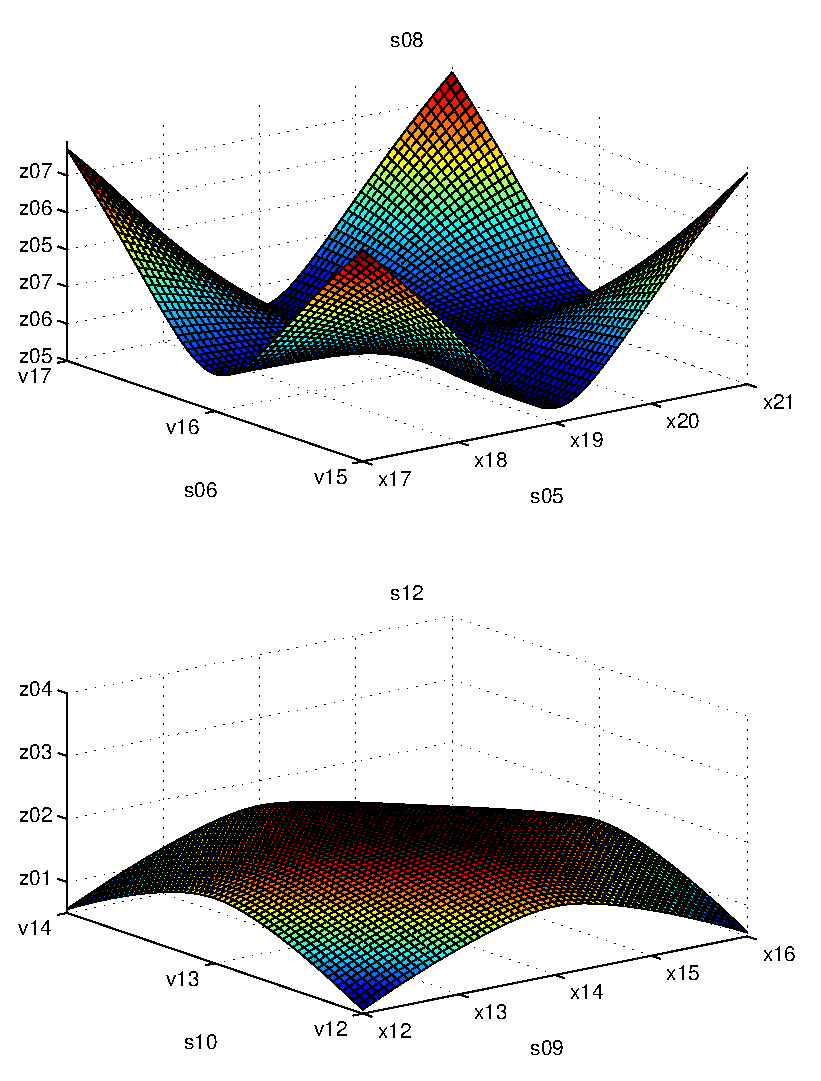
\includegraphics{./Data/Hw3/problem4138.eps}}%
\end{psfrags}%
%
% End problem4138.tex
\end{document}
% See http://www.mathworks.de/matlabcentral/fileexchange/loadFile.do?objectId=4638
% for recent versions of laprint.m.
%
% created by:           LaPrint version 3.16 (13.9.2004)
% created on:           25-Dec-2013 20:10:15
% eps bounding box:     15 cm x 19.6915 cm
% comment:              
%
\begin{psfrags}%
\psfragscanon%
%
% text strings:
\psfrag{s05}[lt][lt]{\fontsize{10}{15}\fontseries{m}\mathversion{normal}\fontshape{n}\selectfont \color[rgb]{0,0,0}\setlength{\tabcolsep}{0pt}\begin{tabular}{l}{$x_1$}\end{tabular}}%
\psfrag{s06}[rt][rt]{\fontsize{10}{15}\fontseries{m}\mathversion{normal}\fontshape{n}\selectfont \color[rgb]{0,0,0}\setlength{\tabcolsep}{0pt}\begin{tabular}{r}{$x_2$}\end{tabular}}%
\psfrag{s08}[b][b]{\fontsize{12}{18}\fontseries{bx}\mathversion{bold}\fontshape{n}\selectfont \color[rgb]{0,0,0}\setlength{\tabcolsep}{0pt}\begin{tabular}{c}$\lambda_1$\end{tabular}}%
\psfrag{s09}[lt][lt]{\fontsize{10}{15}\fontseries{m}\mathversion{normal}\fontshape{n}\selectfont \color[rgb]{0,0,0}\setlength{\tabcolsep}{0pt}\begin{tabular}{l}{$x_1$}\end{tabular}}%
\psfrag{s10}[rt][rt]{\fontsize{10}{15}\fontseries{m}\mathversion{normal}\fontshape{n}\selectfont \color[rgb]{0,0,0}\setlength{\tabcolsep}{0pt}\begin{tabular}{r}{$x_2$}\end{tabular}}%
\psfrag{s12}[b][b]{\fontsize{12}{18}\fontseries{bx}\mathversion{bold}\fontshape{n}\selectfont \color[rgb]{0,0,0}\setlength{\tabcolsep}{0pt}\begin{tabular}{c}$\lambda_2$\end{tabular}}%
%
% axes font properties:
\fontsize{10}{15}\fontseries{m}\mathversion{normal}%
\fontshape{n}\selectfont%
%
% xticklabels:
\psfrag{x01}[t][t]{0}%
\psfrag{x02}[t][t]{0.1}%
\psfrag{x03}[t][t]{0.2}%
\psfrag{x04}[t][t]{0.3}%
\psfrag{x05}[t][t]{0.4}%
\psfrag{x06}[t][t]{0.5}%
\psfrag{x07}[t][t]{0.6}%
\psfrag{x08}[t][t]{0.7}%
\psfrag{x09}[t][t]{0.8}%
\psfrag{x10}[t][t]{0.9}%
\psfrag{x11}[t][t]{1}%
\psfrag{x12}[t][t]{-20}%
\psfrag{x13}[t][t]{-10}%
\psfrag{x14}[t][t]{0}%
\psfrag{x15}[t][t]{10}%
\psfrag{x16}[t][t]{20}%
\psfrag{x17}[t][t]{-20}%
\psfrag{x18}[t][t]{-10}%
\psfrag{x19}[t][t]{0}%
\psfrag{x20}[t][t]{10}%
\psfrag{x21}[t][t]{20}%
%
% yticklabels:
\psfrag{v01}[r][r]{0}%
\psfrag{v02}[r][r]{0.1}%
\psfrag{v03}[r][r]{0.2}%
\psfrag{v04}[r][r]{0.3}%
\psfrag{v05}[r][r]{0.4}%
\psfrag{v06}[r][r]{0.5}%
\psfrag{v07}[r][r]{0.6}%
\psfrag{v08}[r][r]{0.7}%
\psfrag{v09}[r][r]{0.8}%
\psfrag{v10}[r][r]{0.9}%
\psfrag{v11}[r][r]{1}%
\psfrag{v12}[r][r]{-20}%
\psfrag{v13}[r][r]{0}%
\psfrag{v14}[r][r]{20}%
\psfrag{v15}[r][r]{-20}%
\psfrag{v16}[r][r]{0}%
\psfrag{v17}[r][r]{20}%
%
% zticklabels:
\psfrag{z01}[r][r]{-100}%
\psfrag{z02}[r][r]{0}%
\psfrag{z03}[r][r]{100}%
\psfrag{z04}[r][r]{200}%
\psfrag{z05}[r][r]{0}%
\psfrag{z06}[r][r]{20}%
\psfrag{z07}[r][r]{40}%
%
% Figure:
\resizebox{12cm}{!}{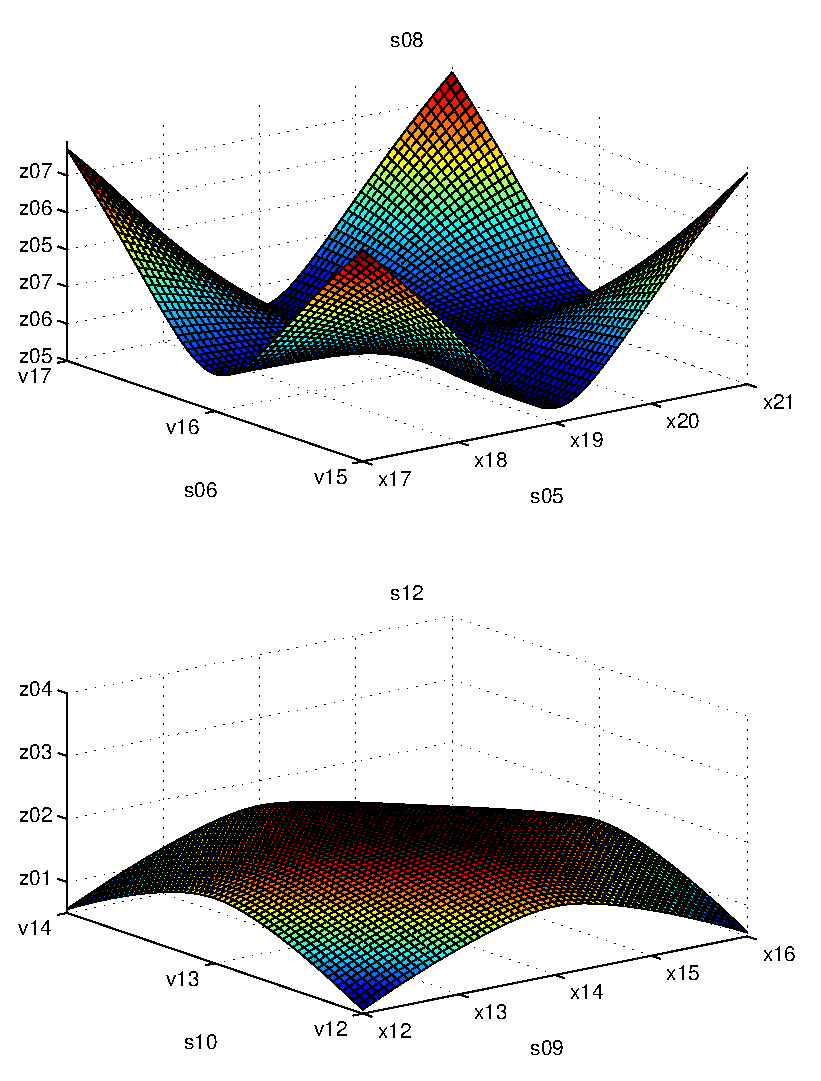
\includegraphics{./Data/Hw3/problem4138.eps}}%
\end{psfrags}%
%
% End problem4138.tex
\end{document}
% See http://www.mathworks.de/matlabcentral/fileexchange/loadFile.do?objectId=4638
% for recent versions of laprint.m.
%
% created by:           LaPrint version 3.16 (13.9.2004)
% created on:           25-Dec-2013 20:10:15
% eps bounding box:     15 cm x 19.6915 cm
% comment:              
%
\begin{psfrags}%
\psfragscanon%
%
% text strings:
\psfrag{s05}[lt][lt]{\fontsize{10}{15}\fontseries{m}\mathversion{normal}\fontshape{n}\selectfont \color[rgb]{0,0,0}\setlength{\tabcolsep}{0pt}\begin{tabular}{l}{$x_1$}\end{tabular}}%
\psfrag{s06}[rt][rt]{\fontsize{10}{15}\fontseries{m}\mathversion{normal}\fontshape{n}\selectfont \color[rgb]{0,0,0}\setlength{\tabcolsep}{0pt}\begin{tabular}{r}{$x_2$}\end{tabular}}%
\psfrag{s08}[b][b]{\fontsize{12}{18}\fontseries{bx}\mathversion{bold}\fontshape{n}\selectfont \color[rgb]{0,0,0}\setlength{\tabcolsep}{0pt}\begin{tabular}{c}$\lambda_1$\end{tabular}}%
\psfrag{s09}[lt][lt]{\fontsize{10}{15}\fontseries{m}\mathversion{normal}\fontshape{n}\selectfont \color[rgb]{0,0,0}\setlength{\tabcolsep}{0pt}\begin{tabular}{l}{$x_1$}\end{tabular}}%
\psfrag{s10}[rt][rt]{\fontsize{10}{15}\fontseries{m}\mathversion{normal}\fontshape{n}\selectfont \color[rgb]{0,0,0}\setlength{\tabcolsep}{0pt}\begin{tabular}{r}{$x_2$}\end{tabular}}%
\psfrag{s12}[b][b]{\fontsize{12}{18}\fontseries{bx}\mathversion{bold}\fontshape{n}\selectfont \color[rgb]{0,0,0}\setlength{\tabcolsep}{0pt}\begin{tabular}{c}$\lambda_2$\end{tabular}}%
%
% axes font properties:
\fontsize{10}{15}\fontseries{m}\mathversion{normal}%
\fontshape{n}\selectfont%
%
% xticklabels:
\psfrag{x01}[t][t]{0}%
\psfrag{x02}[t][t]{0.1}%
\psfrag{x03}[t][t]{0.2}%
\psfrag{x04}[t][t]{0.3}%
\psfrag{x05}[t][t]{0.4}%
\psfrag{x06}[t][t]{0.5}%
\psfrag{x07}[t][t]{0.6}%
\psfrag{x08}[t][t]{0.7}%
\psfrag{x09}[t][t]{0.8}%
\psfrag{x10}[t][t]{0.9}%
\psfrag{x11}[t][t]{1}%
\psfrag{x12}[t][t]{-20}%
\psfrag{x13}[t][t]{-10}%
\psfrag{x14}[t][t]{0}%
\psfrag{x15}[t][t]{10}%
\psfrag{x16}[t][t]{20}%
\psfrag{x17}[t][t]{-20}%
\psfrag{x18}[t][t]{-10}%
\psfrag{x19}[t][t]{0}%
\psfrag{x20}[t][t]{10}%
\psfrag{x21}[t][t]{20}%
%
% yticklabels:
\psfrag{v01}[r][r]{0}%
\psfrag{v02}[r][r]{0.1}%
\psfrag{v03}[r][r]{0.2}%
\psfrag{v04}[r][r]{0.3}%
\psfrag{v05}[r][r]{0.4}%
\psfrag{v06}[r][r]{0.5}%
\psfrag{v07}[r][r]{0.6}%
\psfrag{v08}[r][r]{0.7}%
\psfrag{v09}[r][r]{0.8}%
\psfrag{v10}[r][r]{0.9}%
\psfrag{v11}[r][r]{1}%
\psfrag{v12}[r][r]{-20}%
\psfrag{v13}[r][r]{0}%
\psfrag{v14}[r][r]{20}%
\psfrag{v15}[r][r]{-20}%
\psfrag{v16}[r][r]{0}%
\psfrag{v17}[r][r]{20}%
%
% zticklabels:
\psfrag{z01}[r][r]{-100}%
\psfrag{z02}[r][r]{0}%
\psfrag{z03}[r][r]{100}%
\psfrag{z04}[r][r]{200}%
\psfrag{z05}[r][r]{0}%
\psfrag{z06}[r][r]{20}%
\psfrag{z07}[r][r]{40}%
%
% Figure:
\resizebox{12cm}{!}{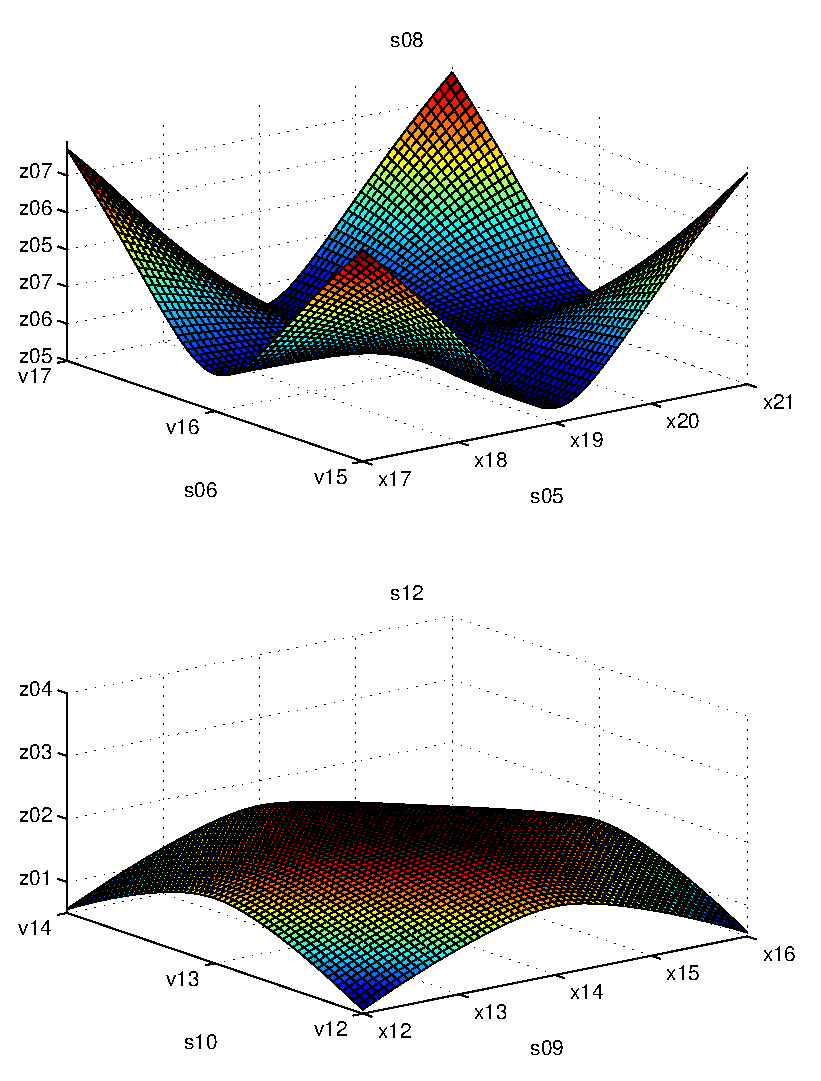
\includegraphics{./Data/Hw3/problem4138.eps}}%
\end{psfrags}%
%
% End problem4138.tex

\caption{Plot of the eigen values of the Hessian of the problem 4.138 with respect to design variables.}
\label{fig:rootsplot}
\end{figure}
\subsection*{Problem 4.150}
The problem of minimum weight deisgn of the symmetric three bar truss system is formulated as follows:\\~\\
Minimize:
\begin{eqnarray*}
f\left(\mathbf x\right) &=& 2\sqrt{2}x_1+x_2
\end{eqnarray*} 
Subject to:
\begin{eqnarray*}
g_1=\frac{1}{2}\left[\frac{P_u}{x_1}+\frac{P_v}{\left(x_1+\sqrt{2}x_2\right)}\right]-20000 &\leq& 0 \\
g_2=\frac{\sqrt{2} P_v}{\left(x_1+\sqrt{2}x_2\right)}-20000 &\leq& 0 \\
g_3=-x_1 &\leq& 0 \\
g_4=-x_2 &\leq& 0
\end{eqnarray*}
where $x_1$ is the cross sectional area of members1 and 3(symmetric structure) and $x_2$ is the cross-sectional area of member  2, $P_u=P \cos{\theta}$,$P_v=P \sin{\theta}$, with $P>0$ and $0\leq \theta \leq 90$. Check for the convexity of the problem for $\theta =60$.
\subsubsection*{Solution}
The cost function of the problem is convex because it is linear in terms of design variables. The constraints $g_3$ and $g_4$ are also convex.
The behavior of constraints $g_1$ and $g_2$ an be determined from their hessian matrix. Hessian matrix of the this two constraints are found as
\begin{eqnarray*}
\triangledown^2g_1=\left[\begin{array}{cc}
\sqrt{2}\left(\frac{P\sin\theta}{\left(x_1+\sqrt{2}x_2\right)^3}+\frac{P\cos\theta}{x_1^3}\right)&{}\frac{2P\sin\theta}{\left(x_1+\sqrt{2}x_2\right)^3}\\{}\frac{2P\sin\theta}{\left(x_1+\sqrt{2}x_2\right)^3}& \frac{2\sqrt{2}P\sin\theta}{\left(x_1+\sqrt{2}x_2\right)^3}
\end{array}\right]
\end{eqnarray*}
~\\~\\~
\begin{eqnarray*}
\triangledown^2g_2=\left[\begin{array}{cc}
\frac{2\sqrt{2}P\sin\theta}{\left(x_1+\sqrt{2}x_2\right)^3}&\frac{4P\sin\theta}{\left(x_1+\sqrt{2}x_2\right)^3}\\ \frac{4P\sin\theta}{\left(x_1+\sqrt{2}x_2\right)^3}& \frac{4\sqrt{2}P\sin\theta}{\left(x_1+\sqrt{2}x_2\right)^3}
\end{array}\right]
\end{eqnarray*}
The Hessian matrices of both the constraints are positive definite for $\theta=\degrees{\frac{\pi}{3}}$ and $x_1 \geq 0$, $x_2\geq 0$. Therefore, the problem is strictly convex.
\subsection*{Problem 8.11}
Determine whether the given direction is descent for the given function.
\begin{eqnarray*}
f\left(\mathbf x\right)=x_1^2+x_2^2+x_3^2 ; \quad \mathbf d=\left(2,4,-2\right)\quad \mathrm{at} \quad \mathbf{x}=\left(1,2,-1\right)
\end{eqnarray*}
\subsubsection*{Solution}
Direction's projection on the gradient's direction should be find in order to determine whether it is a descent direction. Gradient vector is
\begin{eqnarray*}
\mathbf \triangledown f&=&\left[\begin{array}{ccc}
2x_1& 2x_2& 2x_3
\end{array}\right]
\\
&=&\left[\begin{array}{ccc}
2 &4& -2
\end{array}\right]
\end{eqnarray*}
projection of direction on the gradient vector is
\begin{eqnarray*}
\mathbf d&=&\left[\begin{array}{ccc}
2 &4& -2
\end{array}\right]
\\
\mathbf d \cdot  \mathbf \triangledown f &=&\left[\begin{array}{c}
2 \\4\\ -2
\end{array}\right]\left[\begin{array}{ccc}
2 &4& -2
\end{array}\right]=20\\
\mathbf d \cdot  \mathbf \triangledown f &>& 0 
\end{eqnarray*}
Projection of direction on the gradient of the function is found to be positive, therefore, the direction is not descent. 
\subsection*{Problem 8.16}
Find the minimum of the function $f\left(\alpha\right)=7\alpha^2-20\alpha+22$ using equal-interval-search method within accuarcy of 0.001. Use $\delta=0.05$.
\subsubsection*{Solution}
In equal interval equal-interval-search design variable range is determined by $x_l$ and $x_u$ then this range is divided to equal intervals. Function is evaluated at the end of the intervals. A change in function behavior at the interval $k$ is a sign for a root.
\\
\\
For the start of iteration initial values are selected to be as $\alpha_l=1.3$ and $\alpha_u=1.5$. The iterations for the solutions are
\begin{program}
\underline{k=0}
\\
\\
\alpha_l^{(0)}=1.3 \; ,\; \alpha_u^{(0)}=1.5, \delta^{(0)} =0.5\\
\alpha_l^{(0)}=1.3 \; \Longrightarrow f_l^{(0)}=7.83\\
\alpha_1^{(0)}=1.3+0.05 \; \Longrightarrow f_1^{(0)}=7.7575\\
\alpha_2^{(0)}=1.3+0.1 \; \Longrightarrow f_2^{(0)}=7.72\\
\alpha_3^{(0)}=1.3+0.15 \; \Longrightarrow f_3^{(0)}=7.7175\\
\alpha_u^{(0)}=1.3+0.2 \; \Longrightarrow f_u^{(0)}=7.75
\end{program}
\begin{program}
\underline{k=1}
\\
\\
\alpha_l^{(1)}=1.4 \; ,\; \alpha_u^{(1)}=1.5, \delta^{(1)} =0.025\\
\alpha_l^{(1)}=1.4 \; \Longrightarrow f_l^{(1)}=7.72\\
\alpha_1^{(1)}=1.4+0.025 \; \Longrightarrow f_1^{(1)}=7.714375\\
\alpha_2^{(1)}=1.4+0.05 \; \Longrightarrow f_2^{(1)}=7.7175\\
\alpha_3^{(1)}=1.4+0.075 \; \Longrightarrow f_3^{(1)}=7.729375\\
\alpha_u^{(1)}=1.5 \; \Longrightarrow f_u^{(1)}=7.75
\end{program}

\begin{program}
\underline{k=2}
\\
\\
\alpha_l^{(2)}=1.4 \; ,\; \alpha_u^{(2)}=1.45, \delta^{(2)} =0.01\\
\alpha_l^{(2)}=1.4 \; \Longrightarrow f_l^{(2)}=7.72\\
\alpha_1^{(2)}=1.4+0.01 \; \Longrightarrow f_1^{(2)}=7.7167\\
\alpha_2^{(2)}=1.4+0.02 \; \Longrightarrow f_2^{(2)}=7.7148\\
\alpha_3^{(2)}=1.4+0.03 \; \Longrightarrow f_3^{(2)}=7.7143\\
\alpha_4^{(2)}=1.4+0.04 \; \Longrightarrow f_4^{(2)}=7.7152\\
\alpha_u^{(2)}=1.45 \; \Longrightarrow f_u^{(2)}=7.7175
\end{program}
\begin{program}
\underline{k=3}
\\
\\
\alpha_l^{(3)}=1.42 \; ,\; \alpha_u^{(3)}=1.44, \delta^{(3)} =0.005\\
\alpha_l^{(3)}=1.42 \; \Longrightarrow f_l^{(3)}=7.7148\\
\alpha_1^{(3)}=1.42+0.005 \; \Longrightarrow f_1^{(3)}=7.714375\\
\alpha_2^{(3)}=1.42+0.01 \; \Longrightarrow f_2^{(3)}=7.7143\\
\alpha_3^{(3)}=1.42+0.015 \; \Longrightarrow f_3^{(3)}=7.714575\\
\alpha_u^{(3)}=1.44 \; \Longrightarrow f_u^{(3)}=7.7152
\end{program}
\begin{program}
\underline{k=4}
\\
\\
\alpha_l^{(4)}=1.425 \; ,\; \alpha_u^{(4)}=1.435, \delta^{(4)} =0.0025\\
\alpha_l^{(4)}=1.425 \; \Longrightarrow f_l^{(4)}=7.714375\\
\alpha_1^{(4)}=1.425+0.0025 \; \Longrightarrow f_1^{(4)}=7.71429375\\
\alpha_2^{(4)}=1.425+0.005 \; \Longrightarrow f_2^{(4)}=7.7143\\
\alpha_3^{(4)}=1.425+0.0075 \; \Longrightarrow f_3^{(4)}=7.71439375\\
\alpha_u^{(4)}=1.435 \; \Longrightarrow f_u^{(4)}=7.7152
\end{program}
\begin{program}
\underline{k=5}
\\
\\
\alpha_l^{(5)}=1.425 \; ,\; \alpha_u^{(5)}=1.43, \delta^{(5)} =0.001\\
\alpha_l^{(5)}=1.425 \; \Longrightarrow f_l^2=7.714375\\
\alpha_1^{(5)}=1.425+0.001 \; \Longrightarrow f_1^{(5)}=7.714332\\
\alpha_2^{(5)}=1.425+0.002 \; \Longrightarrow f_2^{(5)}=7.714303\\
\alpha_3^{(5)}=1.425+0.003 \; \Longrightarrow f_3^{(5)}=7.714288\\
\alpha_4^{(5)}=1.425+0.004 \; \Longrightarrow f_4^{(5)}=7.734287\\
\alpha_u^{(5)}=1.43 \; \Longrightarrow f_u^{(5)}=7.7143
\end{program}
solution is found as $\alpha^*=1.429$ , $  f^*=7.734287$.
\subsection*{Problem 8.27}
For the following function, direction of change is given. Derive the function of one variable that can be used to determine optimum step size.
\begin{eqnarray*}
f\left(\mathbf x\right)=x_1^2+x_2^2+x_3^2 ; \quad \mathbf d=\left(-2,-4,2\right)\quad \mathrm{at} \quad \mathbf{x}=\left(1,2,-1\right)
\end{eqnarray*}
\subsubsection*{Solution}
Changing the direction of function in the direction $\mathbf d$ by $\alpha$ times at $\mathbf{x}_0$ is given by
\begin{eqnarray*}
\mathbf x=\mathbf{x}_0+\alpha \mathbf d
\end{eqnarray*}
Using problem values, the function for the step size determination is found as
\begin{eqnarray*}
f\left( \mathbf{x}_0+\alpha \mathbf d\right)&=&\left(1-2\alpha\right)^2+\left(2-4\alpha\right)^2+\left(-1+2\alpha\right)^2\\
&=& 4\alpha^2-2\alpha+1+16\alpha^2-16\alpha+4+4\alpha^2-2\alpha+1\\
&=& 24\alpha^2-20\alpha+6\\
\end{eqnarray*}
which should be minimized.
\newpage
\subsection*{Problem 8.53}
\label{Problem1053}
For the following problem complete two iterations of the steepest descent method.
\begin{eqnarray*}
f\left(\mathbf{x}\right)=12.096x_1^2+21.504x_2^2-1.7321x_1-x_2 ; \quad \mathbf x_0 =\left(1,1\right)
\end{eqnarray*}
\subsubsection*{Solution}
Steepest descent algorithm is given by the following steps\\
~\\
\begin{tabular}{lll}
\underline{Step 1} &:& estimate initial value for the design variables and set $\mathbf x_0$ .\\ 
&&\\
 \underline{Step 2} &:& calculate gradient of function $f\left(\mathbf x\right)$ as $\mathbf c^{(k)}=\triangledown f\left(\mathbf x^{(k)}\right)$.\\ 
 &&\\
 \underline{Step 3} &:& calculate length of gradient. If $\lvert \mathbf c\rvert<\epsilon$ then break the iteration and set $\mathbf x^*=\mathbf x^{(k)}$. \\ 
 &&\\
 \underline{Step 4} &:& let the search direction to be $\mathbf d^{(k)}=-\mathbf c^{(k)}$. \\ 
 &&\\
 \underline{Step 5} &:& calculate step size $\alpha$ that minimizes $f\left(\mathbf x^{(k)}+\alpha\mathbf d^{(k)}\right)$. \\ 
 &&\\
 \underline{Step 6} &:& update $\mathbf x^{(k+1)}=\mathbf x^{(k)}+\alpha^{(k)}\mathbf d^{(k)}$ .\\
  &&\\
\underline{Step 7} &:& go to Step 2.
\end{tabular} 
\\
~
\\
~
\\
The iterations for the solution of problem with Steepest Descent Method are given below
\\
~
\\
\underline{For k=0}
\begin{program}
\left(1\right)\quad \mathbf{x}^{(0)}=\left(1,1\right)\ , \, k=0 \ , \ \epsilon=10^{-3}\\~ \\
\left(2\right)\quad \mathbf{c}^{(0)}=\left[22.4599 \ , \ 42.008\right]\\~  \\
\left(3\right)\quad \lvert \mathbf c^{(0)}\rvert=47.6352>\epsilon\\~  \\
\left(4\right)\quad \mathbf d=\left[1.7321-24.192x_1 \ , \ 1-43.008x_2\right]\\~  \\
\left(5\right)\quad f\left(\mathbf x^{(0)}+\alpha^{(0)} \mathbf d^{(0)}\right)=\underbrace{\left(12.096d_1^2+21.504d_2^2\right)}_{\mathrm {\large A}}\alpha^2+ \underbrace{\left(24.192d_1x_1+43.008d_2x_2-1.7321d_1-d_2\right)}_{\mathrm {\large B}}\alpha\\\quad \quad \quad \quad \quad \quad \quad \quad \quad \underbrace{12.096x_1^2+21.504x_2^2-1.7321x_1-x_2}_{\mathrm {\large C}}\\~  \\
\\\quad \quad \quad \quad \quad \quad \quad \quad \quad \delta f=0;2A\alpha+B=0;\\~\\
\quad \quad \quad \quad \quad \quad \quad \quad \quad\Longrightarrow\alpha= \frac{-B}{2A}\\~\\
\quad \quad \quad \quad \quad \quad \quad \quad \quad \alpha=0.0257\\~\\
\left(6\right)\quad \mathbf x^{(1)}=\mathbf x^{(0)}+\mathbf d^{(0)}=\left[0.4215\ , \ -0.0819\right]\\~  \\
\end{program}~
\\
\underline{For k=1}
\begin{program}
\left(2\right)\quad \mathbf{c}^{(1)}=\left[8.4650\ , \ -4.5259\right]\\~  \\
\left(3\right)\quad \lvert \mathbf c^{(1)}\rvert=9.599>\epsilon\\~  \\
\left(4\right)\quad \mathbf d^{(1)}=\left[-8.4650\ , \ 4.5259\right]\\~  \\
\left(5\right)\quad \delta f\left(\mathbf x^{(1)}+\alpha^{(1)} \mathbf d^{(1)}\right)=0\\~  \\
\quad \quad \quad \quad \quad \quad \quad \quad \quad \alpha=0.0230\\~\\
\left(6\right)\quad \mathbf x^{(2)}=\mathbf x^{(1)}+\mathbf d^{(1)}=\left[0.2265\ , \ 0.0222\right]
\end{program}

\subsection*{Problem 8.59}
For the following problem complete two iterations of the Steepest Descent Method.
\begin{eqnarray*}
f\left(\mathbf x\right)&=&9x_1^2+9x_2^2-100\sqrt{x_1^2+x_2^2-20x_2+100}+80\sqrt{x_1^2+x_2^2+20x_2+100}-\\&&5x_1-41x_2 \quad,\quad \mathbf{x}_0=\left(5,2\right)
\end{eqnarray*}
\subsubsection*{Solution}
Steepest Descent Algorithm is given in problem 8.53. Therefore, it is not given here. For the solution, gradient of the cost function is needed which is found as
\begin{eqnarray*}
\mathbf{c}=\mathbf \triangledown f\left(\mathbf x\right)=\left[\begin{array}{c}
18x_1-\frac{100x_1}{\sqrt{x_1^2+x_2^2-20x_2+100}}+\frac{80x_1}{\sqrt{x_1^2+x_2^2+20x_2+100}} \\ 18-x_2-\frac{100x_2-10}{\sqrt{x_1^2+x_2^2-20x_2+100}}+\frac{80x_2+10}{\sqrt{x_1^2+x_2^2-20x_2+100}}-41\end{array}\right]^T
\end{eqnarray*}
Iterations done for the solution is given below,
\\
~
\\
\underline{For k=0}
\begin{program}
\left(1\right)\quad \mathbf{x}^{(0)}=\left(5,2\right)\ , \, k=0 \ , \ \epsilon=10^{-3}\\~ \\
\left(2\right)\quad \mathbf{c}^{(0)}=\left[62.7693 \ , \ 153.6460\right]\\~  \\
\left(3\right)\quad \lvert \mathbf c^{(0)}\rvert=165.9731>\epsilon\\~  \\
\left(4\right)\quad \mathbf d=\left[-62.7693 \ , \ -153.6460\right]\\~  \\
\left(5\right)\quad \delta f\left(\mathbf x^{(0)}+\alpha^{(0)} \mathbf d^{(0)}\right)=0\\~\\
\quad \quad \quad \quad \quad \quad \quad \quad \quad \alpha=0.0669\\~\\
\left(6\right)\quad \mathbf x^{(1)}=\mathbf x^{(0)}+\mathbf d^{(0)}=\left[0.802\ , \ -8.279\right]\\~  \\
\end{program}~
\\
\underline{For k=1}
\begin{program}
\left(2\right)\quad \mathbf{c}^{(1)}=\left[38.8\ , \ -17.5\right]\\~  \\
\left(3\right)\quad \lvert \mathbf c^{(1)}\rvert=42.6>\epsilon\\~  \\
\left(4\right)\quad \mathbf d^{(1)}=\left[-38.8\ , \ 17.5\right]\\~  \\
\left(5\right)\quad \delta f\left(\mathbf x^{(1)}+\alpha^{(1)} \mathbf d^{(1)}\right)=0\\~  \\
\quad \quad \quad \quad \quad \quad \quad \quad \quad \alpha=0.0191\\~\\
\left(6\right)\quad \mathbf x^{(2)}=\mathbf x^{(1)}+\mathbf d^{(1)}=\left[0.063\ , \ -7.9\right]
\end{program}
\subsection*{Problem 8.68}
For the following problem, complete two iterations of the Conjugate Gradient Method.
\begin{eqnarray*}
f\left(\mathbf x\right)&=&9x_1^2+9x_2^2-100\sqrt{x_1^2+x_2^2-20x_2+100}+80\sqrt{x_1^2+x_2^2+20x_2+100}-\\&&5x_1-41x_2 \quad,\quad \mathbf{x}_0=\left(5,2\right)
\end{eqnarray*}
\subsubsection*{Solution}
Conjugate gradient method differs from steepest descent on the way of choosing the search direction. The search direction is chosen as a combination of current gradient and the previous search direction.\newpage ~\\ It's algorithm is
\\
~\\
\begin{tabular}{lll}
\underline{Step 1} &:& estimate initial value for the design variables and set $\mathbf x_0$ .\\ 
&&\\
 \underline{Step 2} &:& compute gradient of function $f\left(\mathbf x\right)$ at current point as $\mathbf c^{(k)}=\triangledown f\left(\mathbf x^{(k)}\right)$.\\ 
 &&\\
 \underline{Step 3} &:& calculate $\lvert \mathbf c^{(k)}\rvert$ ,  if$\lvert \mathbf c^{(k)}\rvert<\epsilon$ then break the iteration and set $\mathbf x^*=\mathbf x^{(k)}$. \\ 
 &&\\
 \underline{Step 4} &:& calculate conjugate search direction as \\ 
  &&\\
  && $\mathbf d^{(k)}=-\mathbf c^{(k)}+\beta^{(k)}\mathbf{d}^{(k-1)}$   \\ 
  &&\\
   &&$\beta ^{(k)}=\left(\frac{\lvert \mathbf c^{(k)}\rvert}{\lvert \mathbf c^{(k-1)}\rvert}\right) $\\
 &&\\
 \underline{Step 5} &:& compute step size $\alpha^{(k)}$ that minimizes $f\left(\mathbf x^{(k)}+\alpha^{(k)}\mathbf d^{(k)}\right)$. \\ 
 &&\\
 \underline{Step 6} &:& update $\mathbf x^{(k+1)}=\mathbf x^{(k)}+\alpha^{(k)}\mathbf d^{(k)}$ .\\
  &&\\
\underline{Step 7} &:& go to Step 2.
\end{tabular} 
\\
~
\\
~
\\
Solution steps of the problem is given below. Before going into the solution its useful to compute gradient of $f$ with respect to design variables.
\begin{eqnarray*}
\mathbf \triangledown f=\left[24.192x_1-1.7321\ , \ 43.008x_2-1\right]
\end{eqnarray*}\\
\underline{For k=0}
\begin{program}
\left(1\right)\quad \mathbf{x}^{(0)}=\left(1,1\right)\ , \, k=0 \ , \ \epsilon=10^{-3}\\~ \\
\left(2\right)\quad \mathbf{c}^{(0)}=\left[22.4599 \ , \ 42.008\right]\\~  \\
\left(3\right)\quad \lvert \mathbf c^{(0)}\rvert=47.6352>\epsilon\\~  \\
\left(4\right)\quad \mathbf d=\left[-22.4599 \ , \ -42.008\right]\\~  \\
\left(5\right)\quad \delta f\left(\mathbf x^{(0)}+\alpha^{(0)} \mathbf d^{(0)}\right)=0\\~\\
\quad \quad \quad \alpha=0.0257\\~\\
\left(6\right)\quad \mathbf x^{(1)}=\mathbf x^{(0)}+\mathbf d^{(0)}=\left[0.4215\ , \ -0.0819\right]
\end{program}
~\\
\underline{For k=1}
\begin{program}
\left(2\right)\quad \mathbf{c}^{(1)}=\left[8.465 \ , \ -4.5259\right]\\~  \\
\left(3\right)\quad \lvert \mathbf c^{(1)}\rvert=9.559>\epsilon\\~  \\
\left(4\right)\quad \mathbf d^{(1)}=-\mathbf c^{(1)}+\beta^{(1)}\mathbf{d}^{(0)}\\~  \\
\quad \quad \ \mathbf d^{(1)}=-\left[8.465 \ , \ -4.5259\right]+ 0.2015 \left[-22.4599 \ , \ 42.008\right]\\~  \\
\quad \quad \quad \  \quad=\left[-12.9909 \ , \ 12.9909 \right] \\~  \\
\left(5\right)\quad \delta f\left(\mathbf x^{(1)}+\alpha^{(1)} \mathbf d^{(1)}\right)=0\\~\\
\quad \quad \quad \alpha=0.01488\\~\\
\left(6\right)\quad \mathbf x^{(2)}=\mathbf x^{(1)}+\mathbf d^{(1)}=\left[0.2294\ , \ 0.1133\right]
\end{program}
\subsection*{Problem 9.10}
For the following problem, complete one iteration of modified Newton's method, aslo check descent condition for the search direction.
\begin{eqnarray*}
f\left(\mathbf x\right)&=&x_1^2+2x_2^2-4x_1-2x_1x_2 \quad ; \quad \mathbf{x}_0=\left(1,1\right)
\end{eqnarray*}
\subsubsection*{Solution}
In modified Newton Algorithm, function to be minimized is expanded to Taylor series that is quadratic in terms of the design variables. Then, the search direction is chosen as the minimizing value of the design variables in the series representation. Because of Hessian is also considered within this method, the converge ratio is quicker than Steepest Descent Method. \\
~\\
Taylor series of a function in quadratic terms is given by
\begin{eqnarray*}
f\left(\mathbf x+\Delta x\right)&=& f\left(\mathbf x\right)+\mathbf c^\mathrm{T} \Delta \mathbf x+\frac{1}{2}\Delta \mathbf x^\mathrm{T}\mathbf H \Delta \mathbf x
\end{eqnarray*}
minimum value of it is found where
\begin{eqnarray*}
\frac{\partial f}{\partial \Delta \mathbf x }=0
\end{eqnarray*}
which results the following relations
\begin{eqnarray*}
\mathbf{c}+\mathbf{H}\Delta \mathbf{x}&=& \mathbf 0\\
\Delta \mathbf{x} &=& -\mathbf{H}^{-1}\mathbf{c}
\end{eqnarray*}
the descent direction is selected to be
\begin{eqnarray*}
\mathbf{d}=\alpha \Delta \mathbf x
\end{eqnarray*}
\newpage ~\\ Modified Newton's Method's algorithm is given below,
\\
~\\
\begin{tabular}{lll}
\underline{Step 1} &:& estimate initial value for the design variables and set $\mathbf x_0$ .\\ 
&&\\
 \underline{Step 2} &:& compute gradient of function $f\left(\mathbf x\right)$ at current point as $\mathbf c^{(k)}=\triangledown f\left(\mathbf x^{(k)}\right)$.\\ 
 &&\\
 \underline{Step 3} &:& calculate $\lvert \mathbf c^{(k)}\rvert$ ,  if$\lvert \mathbf c^{(k)}\rvert<\epsilon$ then break the iteration and set $\mathbf x^*=\mathbf x^{(k)}$. \\ 
 &&\\
 \underline{Step 4} &:& calculate hessian of cost function as\\ 
  &&\\
  && $\mathbf H^{(k)}=-\triangledown^2 f\left(\mathbf x^{(k)}\right)$   \\ 
  &&\\
   &&$\mathbf d^{(k)}=\mathbf {H^{(k)}}^{-1}\mathbf{c}^{(k)} $\\
 &&\\
 \underline{Step 5} &:& compute step size $\alpha^{(k)}$ that minimizes $f\left(\mathbf x^{(k)}+\alpha^{(k)}\mathbf d^{(k)}\right)$. \\ 
 &&\\
 \underline{Step 6} &:& update $\mathbf x^{(k+1)}=\mathbf x^{(k)}+\alpha^{(k)}\mathbf d^{(k)}$ .\\
  &&\\
\underline{Step 7} &:& go to Step 2.
\end{tabular} 
\\
~
\\~\\
Gradient and the Hessian of the problem is found as,

\begin{eqnarray*}
\mathbf{c}=\left[2x_1-2x_2-4 \ , \ 4x_2-2x_1\right] \ , \ \mathbf{H}=\left[\begin{array}{cc}
2 & -2 \\
-2 & 4\end{array}\right]
\end{eqnarray*}
The iterations of the problem is given below.\\~\\
\underline{For k=0}
\begin{program}
\left(1\right)\quad \mathbf{x}^{(0)}=\left(1,1\right)\ , \, k=0 \ , \ \epsilon=10^{-3}\\~ \\
\left(2\right)\quad \mathbf{c}^{(0)}=\left[-4 \ , \ 2\right]\\~  \\
\left(3\right)\quad \lvert \mathbf c^{(0)}\rvert=4.2426>\epsilon\\~  \\
\left(4\right)\quad \mathbf d=\mathbf {H^{(0)}}^{-1}\mathbf{c}^{(0)}\\~  \\
\quad \quad \quad \ = \left[\begin{array}{cc}1 & 0.5 \\ 0.5 & 0.5 \end{array}\right]\left[\begin{array}{c}-4 \\ 2\end{array}\right]=\left[\begin{array}{c}-3 \\ -1\end{array}\right]\\~  \\
\quad \quad \quad \ -{\mathbf{c}^{(0)}}^{\mathrm T} \mathbf {H^{(0)}}\mathbf{c}^{(0)}<0 \Longrightarrow \text{descent direction} \\~\\
\left(5\right)\quad \delta f\left(\mathbf x^{(0)}+\alpha^{(0)} \mathbf d^{(0)}\right)=0\\~\\
\quad \quad \quad \alpha=-1\\~\\
\left(6\right)\quad \mathbf x^{(1)}=\mathbf x^{(0)}+\mathbf d^{(0)}=\left[4\ , \ 2\right]
\end{program}
\subsection*{Problem 9.12}
For the following problem, complete two iterations of Davidon-Fletcher-Powel method, also check descent condition for the search direction.
\begin{eqnarray*}
f\left(\mathbf x\right)&=&x_1^2+2x_2^2-4x_1-2x_1x_2 \quad ; \quad \mathbf{x}_0=\left(1,1\right)
\end{eqnarray*}
\subsubsection*{Solution}
Davidon-Fletcher-Powel method differs from Generalized Newton Method only on the calculation of the Hessian of the cost function. In this algorithm inverse of the Hessian is approximated and calculated by the approximation in the previous step.
\\~\\
 Davidon-Fletcher-Powel algorithm is given below,
\\
~\\
\begin{tabular}{lll}
\underline{Step 1} &:& estimate initial value for the design variables $\mathbf x_0$ and inverse of Hessian $\mathbf{A}^{(0)}$.\\ 
&&\\
 \underline{Step 2} &:& compute gradient of function $f\left(\mathbf x\right)$ at current point as $\mathbf c^{(k)}=\triangledown f\left(\mathbf x^{(k)}\right)$.\\ 
 &&\\
 \underline{Step 3} &:& calculate $\lvert \mathbf c^{(k)}\rvert$ ,  if$\lvert \mathbf c^{(k)}\rvert<\epsilon$ then break the iteration and set $\mathbf x^*=\mathbf x^{(k)}$. \\ 
 &&\\
 \underline{Step 4} &:& calculate search direction as\\ 
  &&\\
  && $\mathbf d^{(k)}={\mathbf{A}^{(k)}} \mathbf{c}^{(k)}$   \\ 
 &&\\
 \underline{Step 5} &:& compute step size $\alpha^{(k)}$ that minimizes $f\left(\mathbf x^{(k)}+\alpha^{(k)}\mathbf d^{(k)}\right)$. \\ 
 &&\\
 \underline{Step 6} &:& update $\mathbf x^{(k+1)}=\mathbf x^{(k)}+\alpha^{(k)}\mathbf d^{(k)}$ and calculate $\mathbf{A}^{(k+1)}, \mathbf{B}^{(k)}, \mathbf{C}^{(k)}$\\
  &&\\
\underline{Step 7} &:& go to Step 2.
\end{tabular} 
\\
~
\\~\\
The problem solution steps are given below.
~\\~\\
\underline{For k=0}
\begin{program}
\left(1\right)\quad \mathbf{x}^{(0)}=\left(1,1\right)\ , \, k=0 \ , \ \epsilon=10^{-3}\ , \ \mathbf{A}^{(0)}=\left[\begin{array}{cc}1 & 0 \\0 &1\end{array}\right] \\~ \\
\left(2\right)\quad \mathbf{c}^{(0)}=\left[-4 \ , \ 2\right]\\~  \\
\left(3\right)\quad \lvert \mathbf c^{(0)}\rvert=4.2426>\epsilon\\~  \\
\left(4\right)\quad \mathbf d=\mathbf {A}^{(0)}\mathbf{c}^{(0)}\\~  \\
\quad \quad \quad \ = \left[\begin{array}{cc}1 & 0 \\ 0& 1 \end{array}\right]\left[\begin{array}{c}-4 \\ 2\end{array}\right]=\left[\begin{array}{c}-4\\ 2\end{array}\right]\\~  \\
\left(5\right)\quad \delta f\left(\mathbf x^{(0)}+\alpha^{(0)} \mathbf d^{(0)}\right)=0\\~\\
\quad \quad \quad \alpha=-0.25\\~\\
\left(6\right)\quad \mathbf x^{(1)}=\mathbf x^{(0)}+\alpha^{(0)}\mathbf d^{(0)}=\left[2\ , \ 0.5\right]\\~  \\
\quad \quad \ \  \mathbf{A}^{(1)} = \mathbf{A}^{(0)}+\mathbf{B}^{(0)}+\mathbf{C}^{(0)}\\~  \\
\quad \quad \ \ \mathbf{y}^{(0)}=\mathbf{c}^{(1)}-\mathbf{c}^{(0)}=\left[\begin{array}{c}3\\ -4\end{array}\right]\\~  \\
\quad \quad \ \ \mathbf{z}^{(0)}={\mathbf A }^{(0)}\mathbf{y}^{(0)}=\left[\begin{array}{c}3\\ -4\end{array}\right]\\~  \\
\quad \quad \ \ \mathbf{s}^{(0)}=\alpha\mathbf{d}^{(0)}=\left[\begin{array}{c}1\\ -0.5\end{array}\right]\\~  \\
\quad \quad \ \ \mathbf{B}^{(0)}=\frac{\mathbf{s}^{(0)}{\mathbf{s}^{\mathrm{T}}}^{(0)}}{\mathbf{s}^{(0)}{\mathbf{y}}^{(0)}}=\left[\begin{array}{cc}0.2&-0.1\\ -0.1 &0.05\end{array}\right]\\~  \\
\quad \quad \ \ \mathbf{C}^{(0)}=-\frac{\mathbf{z}^{(0)}{\mathbf{z}^{\mathrm{T}}}^{(0)}}{\mathbf{y}^{(0)}{\mathbf{z}}^{(0)}}=\left[\begin{array}{cc}-0.36&-0.48\\ 0.48 &-0.64\end{array}\right]\\~  \\
\quad \quad \ \  \mathbf{A}^{(1)} =\left[\begin{array}{cc}0.84&-0.38\\ 0.38 &0.41\end{array}\right]
\end{program}
\underline{For k=1}
\begin{program}
\left(2\right)\quad \mathbf{c}^{(1)}=\left[-1 \ , \ 2\right]\\~  \\
\left(3\right)\quad \lvert \mathbf c^{(1)}\rvert=2.2361>\epsilon\\~  \\
\left(4\right)\quad \mathbf d= {\mathbf A}^{(1)}\mathbf{c}^{(1)}\\~  \\
\quad \quad \quad \ = \left[\begin{array}{cc}0.84 & 0.38 \\ -0.38& 0.41 \end{array}\right]\left[\begin{array}{c}-1 \\ -2\end{array}\right]=\left[\begin{array}{c}-0.13\\ 1.2\end{array}\right]\\~  \\
\left(5\right)\quad \delta f\left(\mathbf x^{(1)}+\alpha^{(1)} \mathbf d^{(1)}\right)=0\\~\\
\quad \quad \quad \alpha=0.3537\\~\\
\left(6\right)\quad \mathbf x^{(1)}=\mathbf x^{(1)}+\alpha^{(1)} \mathbf d^{(1)}=\left[1.954\ , \ 0.9244\right]\\~  \\
\quad \quad \ \  \mathbf{A}^{(2)} = \mathbf{A}^{(1)}+\mathbf{B}^{(1)}+\mathbf{C}^{(1)}\\~  \\
\quad \quad \ \ \mathbf{y}^{(1)}=\mathbf{c}^{(2)}-\mathbf{c}^{(1)}=\left[\begin{array}{c}2.0591\\-2.2103\end{array}\right]\\~  \\
\quad \quad \ \ \mathbf{z}^{(1)}={\mathbf A }^{(1)}\mathbf{y}^{(1)}=\left[\begin{array}{c}0.9927\\-1.6887\end{array}\right]\\~  \\
\quad \quad \ \ \mathbf{s}^{(1)}=\alpha^{(1)}\mathbf{d}^{(1)}=\left[\begin{array}{c}-0.0460\\ 0.4244\end{array}\right]\\~  \\
\quad \quad \ \ \mathbf{B}^{(1)}=\frac{\mathbf{s}^{(1)}{\mathbf{s}^{\mathrm{T}}}^{(1)}}{\mathbf{s}^{(1)}{\mathbf{y}}^{(1)}}=\left[\begin{array}{cc}-0.0092&0.0849\\0.0849&-0.7836\end{array}\right]\\~  \\
\quad \quad \ \ \mathbf{C}^{(1)}=-\frac{\mathbf{z}^{(1)}{\mathbf{z}^{\mathrm{T}}}^{(1)}}{\mathbf{y}^{(1)}{\mathbf{z}}^{(1)}}=\left[\begin{array}{cc}0.5888&-0.4210\\-0.4210 & 0.3010\end{array}\right]\\~  \\
\quad \quad \ \  \mathbf{A}^{(2)} =\left[\begin{array}{cc}    1.4696 &   0.0439\\-0.7161& -0.0726\end{array}\right]
\end{program}
\subsection*{Problem 9.33}
For the following problem, complete two iterations of BFGS method.
\begin{eqnarray*}
f\left(\mathbf x\right)&=&x_1^2+2x_2^2-4x_1-2x_1x_2 \quad ; \quad \mathbf{x}_0=\left(1,1\right)
\end{eqnarray*}
\subsubsection*{Solution}
BFGS method differs from Davidon-Fletcher-Powel from only usage approximation of Hessian rather than approximation of inverse of Hessian.\\~\\
\newpage
~\\BFGS algorithm is as follows
\\
~\\
\begin{tabular}{lll}
\underline{Step 1} &:& estimate initial value for the design variables $\mathbf x_0$ and inverse of Hessian $\mathbf{A}^{(0)}$.\\ 
&&\\
 \underline{Step 2} &:& compute gradient of function $f\left(\mathbf x\right)$ at current point as $\mathbf c^{(k)}=\triangledown f\left(\mathbf x^{(k)}\right)$.\\ 
 &&\\
 \underline{Step 3} &:& calculate $\lvert \mathbf c^{(k)}\rvert$ ,  if$\lvert \mathbf c^{(k)}\rvert<\epsilon$ then break the iteration and set $\mathbf x^*=\mathbf x^{(k)}$. \\ 
 &&\\
 \underline{Step 4} &:& calculate search direction from the equation\\ 
  &&\\
  && ${\mathbf{H}^{(k)}}\mathbf d^{(k)}= \mathbf{c}^{(k)}$   \\ 
 &&\\
 \underline{Step 5} &:& compute step size $\alpha^{(k)}$ that minimizes $f\left(\mathbf x^{(k)}+\alpha^{(k)}\mathbf d^{(k)}\right)$. \\ 
 &&\\
 \underline{Step 6} &:& update $\mathbf x^{(k+1)}=\mathbf x^{(k)}+\alpha^{(k)}\mathbf d^{(k)}$ and calculate $\mathbf{H}^{(k+1)}, \mathbf{D}^{(k)}, \mathbf{E}^{(k)}$\\
  &&\\
\underline{Step 7} &:& go to Step 2.
\end{tabular} 
~\\~\\
Iterations of BFGS solution of the problem is given below,\\
~\\
\underline{For k=0}
\begin{program}
\left(1\right)\quad \mathbf{x}^{(0)}=\left(1,1\right)\ , \, k=0 \ , \ \epsilon=10^{-3}\ , \ \mathbf{H}^{(0)}=\left[\begin{array}{cc}1 & 0 \\0 &1\end{array}\right] \\~ \\
\left(2\right)\quad \mathbf{c}^{(0)}=\left[-4 \ , \ 2\right]\\~  \\
\left(3\right)\quad \lvert \mathbf c^{(0)}\rvert=4.2426>\epsilon\\~  \\
\left(4\right)\quad \mathbf d={\mathbf{H}^{-1}}^{(0)}\mathbf{c}^{(0)}\\~  \\
\quad \quad \quad \ = \left[\begin{array}{cc}1 & 0 \\ 0& 1 \end{array}\right]\left[\begin{array}{c}-4 \\ 2\end{array}\right]=\left[\begin{array}{c}-4\\ 2\end{array}\right]\\~  \\
\left(5\right)\quad \delta f\left(\mathbf x^{(0)}+\alpha^{(0)} \mathbf d^{(0)}\right)=0\\~\\
\quad \quad \quad \alpha=-0.25\\~\\
\left(6\right)\quad \mathbf x^{(1)}=\mathbf x^{(0)}+\alpha^{(0)}\mathbf d^{(0)}=\left[2\ , \ 0.5\right]\\~  \\
\quad \quad \ \  \mathbf{H}^{(1)} = \mathbf{H}^{(0)}+\mathbf{D}^{(0)}+\mathbf{E}^{(0)}\\~  \\
\quad \quad \ \ \mathbf{y}^{(0)}=\mathbf{c}^{(1)}-\mathbf{c}^{(0)}=\left[\begin{array}{c}3\\ -4\end{array}\right]\\~  \\
\quad \quad \ \ \mathbf{s}^{(0)}=\alpha\mathbf{d}^{(0)}=\left[\begin{array}{c}1\\ -0.5\end{array}\right]\\~  \\
\quad \quad \ \ \mathbf{D}^{(0)}=\frac{\mathbf{y}^{(0)}{\mathbf{y}^{\mathrm{T}}}^{(0)}}{\mathbf{y}^{(0)}{\mathbf{s}}^{(0)}}=\left[\begin{array}{cc}    0.2000 &  -0.1000\\-0.1000&    0.0500\end{array}\right]\\~  \\
\quad \quad \ \ \mathbf{E}^{(0)}=\frac{\mathbf{c}^{(0)}{\mathbf{c}^{\mathrm{T}}}^{(0)}}{\mathbf{c}^{(0)}{\mathbf{d}}^{(0)}}=\left[\begin{array}{cc}      5.4795  & -2.7397\\   -2.7397 &   1.3699\end{array}\right]\\~  \\
\quad \quad \ \  \mathbf{H}^{(1)} =\left[\begin{array}{cc}8.2795   &-5.1397\\  -5.1397  &  5.5699\end{array}\right]
\end{program}
\underline{For k=1}
\begin{program}
\left(2\right)\quad \mathbf{c}^{(1)}=\left[-1 \ , \ -2\right]\\~  \\
\left(3\right)\quad \lvert \mathbf c^{(1)}\rvert= 2.2361>\epsilon\\~  \\
\left(4\right)\quad {\mathbf{H}}^{(1)}\mathbf d=\mathbf{c}^{(1)}\\~  \\
\quad \quad \quad \ \mathbf d^{(1)}=\left[\begin{array}{c}   -0.8046 \\ -1.1015\end{array}\right]\\~  \\
\left(5\right)\quad \delta f\left(\mathbf x^{(1)}+\alpha^{(1)} \mathbf d^{(1)}\right)=0\\~\\
\quad \quad \quad \alpha=-1.1555\\~\\
\left(6\right)\quad \mathbf x^{(2)}=\mathbf x^{(1)}+\alpha^{(1)}\mathbf d^{(1)}=\left[-0.3110 \ , \ -0.0777\right]\\~  \\
\quad \quad \ \  \mathbf{H}^{(2)} = \mathbf{H}^{(1)}+\mathbf{D}^{(1)}+\mathbf{E}^{(1)}\\~  \\
\quad \quad \ \ \mathbf{y}^{(1)}=\mathbf{c}^{(2)}-\mathbf{c}^{(1)}=\left[\begin{array}{c}     2.9297\\1.7728\end{array}\right]\\~  \\
\quad \quad \ \ \mathbf{s}^{(1)}=\alpha^{(1)}\mathbf{d}^{(1)}=\left[\begin{array}{c}   0.9297\\1.2728\end{array}\right]\\~  \\
\quad \quad \ \ \mathbf{D}^{(1)}=\frac{\mathbf{y}^{(1)}{\mathbf{y}^{\mathrm{T}}}^{(1)}}{\mathbf{y}^{(1)}{\mathbf{s}}^{(1)}}=\left[\begin{array}{cc}-0.2045  &  0.9632\\ 0.9632 &  -4.5369\end{array}\right]\\~  \\
\quad \quad \ \ \mathbf{E}^{(1)}=\frac{\mathbf{c}^{(1)}{\mathbf{c}^{\mathrm{T}}}^{(1)}}{\mathbf{c}^{(1)}{\mathbf{d}}^{(0)}}=\left[\begin{array}{cc}      0.3325 &   0.6650\\  0.6650   & 1.3300\end{array}\right]\\~  \\
\quad \quad \ \  \mathbf{H}^{(1)} =\left[\begin{array}{cc}     8.4075 &  -3.5115\\-3.5115 &   2.3630\end{array}\right]
\end{program}
~\\
Approximation of Hessian is getting closer to the real Hessian of the cost function by subsequent iterations.

\bibliographystyle{plain}
\bibliography{bibliograph}
\end{document} 
